\documentclass{book}

\usepackage[headings]{fullpage}
%\usepackage{scribe}

% Packages
\usepackage{amsfonts}
\usepackage{amsmath}
\usepackage{amsthm}
%\usepackage[letterpaper,margin=1in]{geometry}
\usepackage{graphics}
\usepackage{epsfig}
\usepackage{color}
\usepackage{array}
\usepackage{pstricks}
\usepackage{pst-plot}
\usepackage{multirow}
%\usepackage{pstricks-add}


\title{CSE103: Probability and Statistics}
\author{Sanjoy Dasgupta \and Yoav Freund}
\theoremstyle{plain}
\newtheorem{lemma}{Lemma}
\newtheorem{claim}[lemma]{Claim}
\newtheorem{theorem}[lemma]{Theorem}
\newtheorem{corollary}[lemma]{Corollary}
\newtheorem{prop}[lemma]{Property}

\theoremstyle{definition}
\newtheorem{define}[lemma]{Definition}
\newtheorem{example}[lemma]{Example}

\newtheorem{problem}{Problem}

\newcommand{\E}{\mathbb{E}}
\newcommand{\R}{\mathbb{R}}
\newcommand{\U}{\mathbb{U}}
\newtheorem{fact}[lemma]{Fact}

\newcommand{\bP}{\mathbb{P}}
\newcommand{\var}{\mbox{\rm var}}
\newcommand{\pr}{\mbox{\rm Pr}}

\def\X{{\cal X}}
\def\cost{{\mbox{\rm cost}}}



\begin{document}

\maketitle
\tableofcontents
\chapter{Introduction}

What is ``probability''? What is ``statistics''? Why are they
important?

This introductory chapter is a gentle introduction to these concepts,
in later chapters we will go deeper and provide you with specific
tools for solving specific problems.

This chapter provides a high level panorama for the rest of the book,
sit back and enjoy!

\section{AB tests of online ads}

Suppose you own a web site and that you make money by placing
advertisements on the pages of our site. The way advertisers pay the web
site is based on ``click through'' events (CT)\footnote{Actually, CTs are
  only part of the payment contract, there are many other factors that effect
  the payment. For simplicity we concentrate here on CTs.} 
A CT is the event that a particular ad is displayed on a
web page (also called an {\em impression}) and the user clicks on the
ad to go to the advertiser's site. That click is an indication of some
interest on the part of the visitor. You, the wbsite owner, get
payed when whenever a CT occurs.

For simplicity, let's consider a single static page, with a single
location on the page for presenting the advertisement and just two
alternative ads to place in this location, which we will call ad A and
ad B. 

How can we figure out which is the best advertisement to put on the
page?

One thing we can do is this: each time the web page is presented,
choose one of the possible ads in an alternating manner
(B,A,B,A,B,... ) and present the page to the visitor. We then see if
the visitor clicks on the advertisement, producing a CT. Suppose that
the number of visitors to the page is very large. The {\em law of
  large numbers} tells us that the fraction of CTs among all the
impressions of A (or B) converges to a particular limit.  This number
is called the ``click through rate'' or CTR for the ad. If the
paymnent for all ads are equal then the ad with the highest CTR is the
best one to place on the page.

The law of large numbers is a fundamental law of probability and
statistics, we will come back to it later.

\iffalse
This is an example of {\em Statistical inference}. Statistical
inference is a set of methods for analyzing collected data and drawing
conclusions about the real world from that data. 
\fi

A single page-visit, together with a flag indicating whether or not
the ad was clicked is called an {\em observation} or an {\em outcome}
and the sequence of $n$ independent observations is called a {\em
  sample}. Statistics is a set of methods for drawing conclusions from
random samples. The process that is generating the observations is
called a {\em Stochastic Process}. The conclusions we draw are stated
as properties of this stochastic process. In our case, we conclude
that one ad has a higher CTR than the other.

Suppose first we have 10,000 impressions for each of the two ads, and
suppose we got 200 CTs for ad A and 150 CTs for ad B. All other things
being equal, we can conclude the the CTR for ad A is about \%$2$ and for
ad B is about \%$1.5$ and our preference should be to present
ad A rather than ad B. However, it is intuitively clear that this
conclusion is not a very confident one, as it rests on a difference of
one in the number of CTs.

As we cannot make a confident conclusions, we continue placing the ads
in an alternating order (A,B,A,B,...) until we have 1,000,000
impressions of each type. Suppose at that point that we have 200,000
CTs for A and 150,000 CT's for B. The CTR's are the same as before:
\%$1.6$ for A and  \%$1.5$  for B. Again, we conclude that A is a
better ad than B. In this case the difference in
the number of CTs is 50,000 rather than 50 and our intuition tells us
that we can be confident that A is the ad with the higher CTR.

How can we justify this intuition?

To explain and quantify this intuition we use probability theory.

\section{Probability Theory}

Probability theory is a branch of mathematics which is the foundation
for statistics. This is similar to the way in which discrete math and
the theory of computation are the foundation for writing correct and
efficient computer programs.

The input for statistical inference is data collected from the real
world, the output is a {\em model} of the real world. Probability
theory works in the opposite direction. The input is a {\em stochastic
  process} or a {\em model}, and the output are probabilities of {\em
  events}.

Specifically, in our case, we can model the process generating the
click-through observation using two biased coins. An {\em unbiased
  coin} is a symmetric coin for which the probability of landing
``heads'' is equal to the probability of landing ``tails''.  A {\em
  biased} coin is one where these probabilities are different.  In our
case the coin for ad A has probability $p_A$ of landing ``heads''
which is equal to the probability that a random visitor will click on
the ad. Similarly $p_B$ corresponds to the probability that the coin B
lands ``heads'' which is equal to the probability that a random
visitor will click on the ad B. More succinctly, $P_A$ is the CTR of
ad A and $P_B$ is the CTR is ad B.

The question that we want to answer is which probability is larger, is
$P_A>P_B$ or is the reverse true: $P_B \leq P_B$ ?

Suppose we are are in the first case in which we presented each
advertisement $10,000$ times and got $200$ click-throughs for ad A and
$150$ for ad B. Clearly, it seems that $P_A>P_B$. But how {\em
  confident} can we be that this is indeed the case?

To answer this question we consider two alternative {\em statistical
hypotheses}: the first is that $P_A>P_B$, the second is that $P_A
\leq P_B$. 

We then find the two settings of $P_A$ and $P_B$ that conform with
each hypothesis and give the highest probability for the data.  For
the hypothesis $P_A>P_B$ we get the highest probability when
$P_A=0.02,P_B=0.015$. For the alternative hypothesis we use
$P_A=0.0175,P_B=0.0175$, i.e. we place the two probabilities midway
between the two observed rates.\footnote{Strictly speaking the
  mid-point is not the highest probability setting, but the difference
  is small and we ignore it here.}.

We now compute the probability of the observed data corresponding to
each of these two settings, which correspond to the two alternative
hypotheses. Clearly the probability of the data under the first
settings will be higher than the probability of the second, so if we
take the ratio of the two probabilities we expect to get a number
smaller than 1. The question is, how much smaller than 1?

Computing this ratio is not a trivial matter. You will learn how to
do it later in the course. For now, I'll tell you that when the number
of impressions for each ad is 10,000 the ratio is $0.6766$, while when
the number of impressions is 1,000,000 the ratio is smaller than
$10^{-16} = 1/10,000,000,000,000,000$. In other words, in the first
case we cannot conclude which ad is better with any degree of
confidence, while in the second case we can be pretty sure that the
first ad is better.

Note how dramatic is the improvement in confidence, increasing the
sample size from 10,000 to 1,000,000 transforms a relative gap of 5\%
from an insignificant gap to one from which can conclude something
almost surely. Keep this very small number $10^{-16}$ in mind, we will
get back to it later in the course.

\section{Low probability vs. certainty}
In computer science we are used to giving absolute guarantees: we
expect that hardware and software will give the correct answer each 
and every time. The whole concept of ``debugging'' a program is based
on the assumption that every mistake can be traced back to a
particular part of the computer code and thereby eliminated. 

However, in the real world, many computer errors cannot be
reconstructed, explained, or corrected. The more realistic goal is
becoming to have computer systems that minimize the number of errors
without necessarily correcting all of the bugs.

Certainty is golden, however, in the real world, having a guarantee
that some error will occur no more than once every $10^{16}$ attempts
is a very strong guarantee. Increasing $n$ from $1,000,000$ to
$100,000,000$ will reduce the probability to 1 in $10^{64}$.

\section{Average and Mean}
The number of observations, or the size of the sample $n$ is of
central importance in probability and in statistics. In general, as
$n$ increases we reach the ``law of large numbers'' which tells us
that averages converge to the means.

People sometimes use ``mean'' and ``average'' interchangeably. However
in probability and statistics the difference is very important. Going back to the
click-through example above. consider the sequence of presentations of
the ad A, each resulting either in a click (1) or in a non-click
(0). For example, suppose the sequence is:
\[
0,0,0,1,0,0,0,0,1,1,0,0,0,0,0,0,0,1,0,0,0,0,0,0,...
\] 
The {\em average} of the first 5 outcomes is $1/5$. If we compute
the average of the first $n$ outcome for $n=1,2,3,...$ we get a
sequence of {\em running averages}:
\[
0,0,0,1/3,1/4,1/5,1/6,1/7,2/8,3/9,3/10,3/11,...
\]
As the sequence of outcomes is random, the sequence of averages is
also random. By this we mean that if we collected a difference
sequence of observations from the same source, we are very likely to
get a different sequence. In the language of probability, we say that
the outcomes and the averages are {\em random variables}.

The terms: ``empirical'', ``observational'', ``sample'', ``random
variable'' indicate that the quantity we are referring to is likely to
change if we repeat the same experiment.

The mean, on the other hand, is {\em not} a random variable. The mean
is a {\em constant property of the source}, in this case, the mean is
equal to $P_A,P_B$ which are the CTRs for ad A and ad B
respectively. In fact $P_A$ and $P_B$ are the quantities that
determine which ad is more profitable.\footnote{Other terms that are
  used to refer to the average are the {\em empirical mean} or the
  {\em sample mean}. These can be easily confused with the regular
  mean. However, they are random variables, not constants.}

The law of large numbers connects the sequence of running averages and
the mean. What the law of large number says (roughly) is that the
sequence of averages converges to the mean. In other words, if $n$ is
large enough, the difference between the average and the mean is going
to be small with high probability.

\section{Monte-carlo simulations}
As I said above, computing the probability flipping a biased coin $n$
times will result in $k$ heads and $n-k$ tails is not
trivial and requires some knowledge of probability theory. However,
symbolic derivation (also called ``closed form solution'') is not the
only way to arrive at the answer. There is another way which is called
``monte-carlo simulations''.

A monte-carlo simulation is a computer program that simulates the
process of generating the outcomes. It uses ``pseudo-random number
generators'' about which we will learn later on. For now it suffices
to describe the pseudo-random number generator as a function {\tt
  random(p)}. Every time {\tt random(p)} is called it returns a bit
whose value is $1$ with probability $p$ and $0$ with probability
$1-p$.

\begin{figure}[p]
\begin{center}
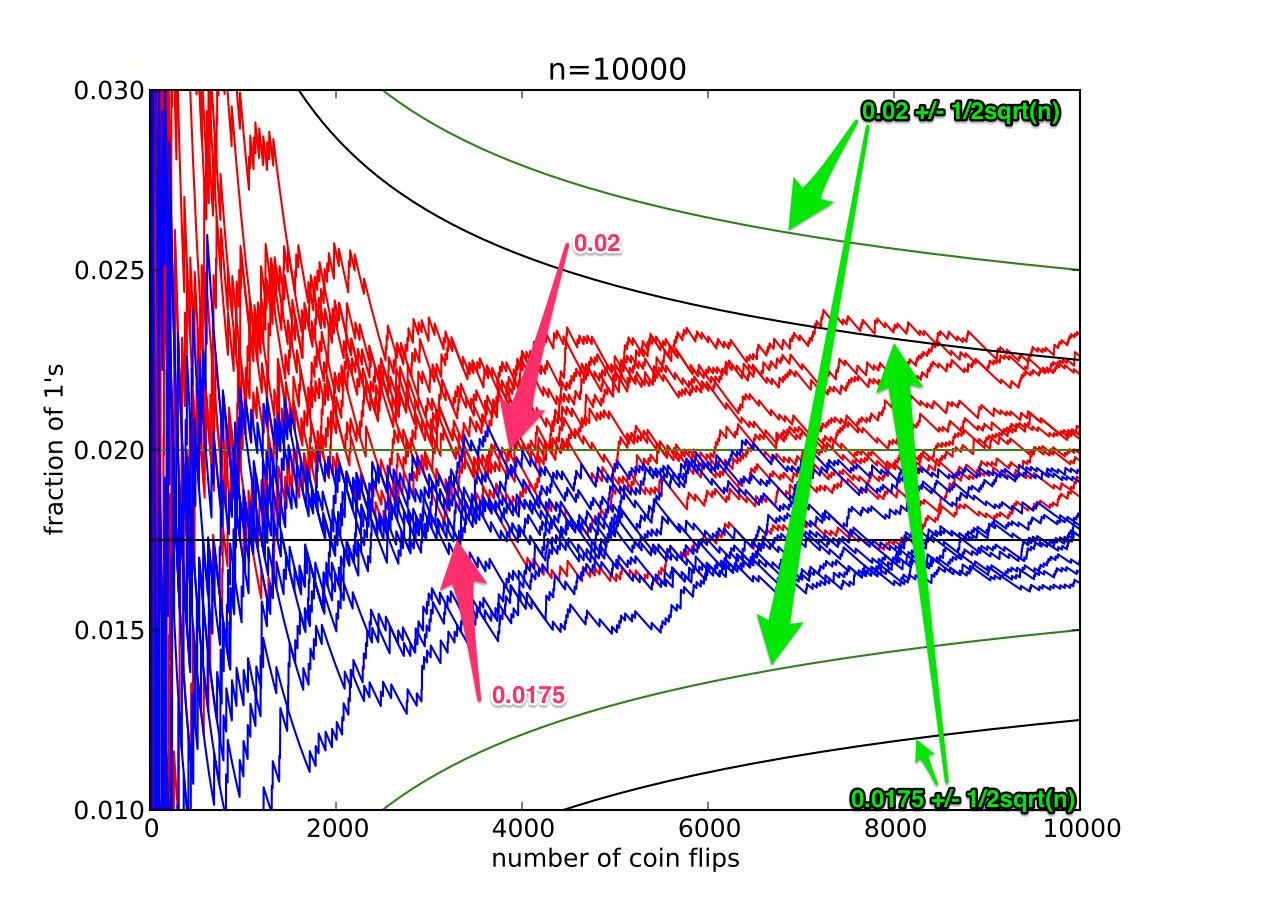
\includegraphics[width=5in]{figs/averages10000.png}
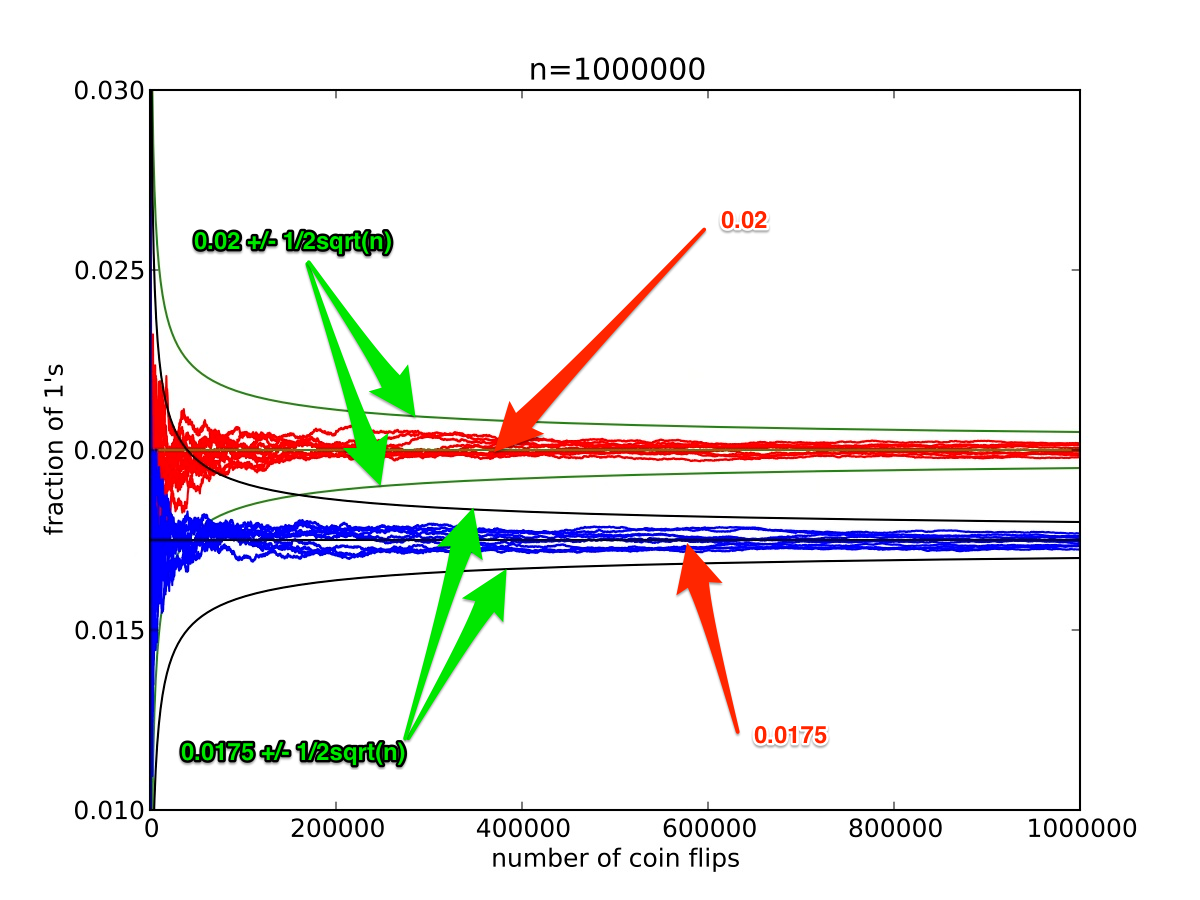
\includegraphics[width=5in]{figs/averages1000000.png}
\end{center}
\caption{\label{fig:Averages} Trajectories of running averages of
  random sequences generated by a biased coin with sides that say
  ``0'' and ``1''. There are two sets of 10 trajectories. The red
  trajectories correspond to sequences of random coin flips where the
  probability of 1 is $0.02$. The blue trajectories correspond to
  sequences of random coin flips where the probability of a 1 is
  $0.0175$}
\end{figure}

Using a random number generator we can create samples of the type
described above, compute running averages of these sample, and plot
them, see Figure~\ref{fig:Averages}.\footnote{The code is available
  via GitHub: {\tt
    https://github.com/yoavfreund/CSE103-code/blob/master/MonteCarlo/monteCarlo.py}}
These plots demostrate why there is such a qualitative difference
between a sample of size $10,000$ and a sample of size
$1,000,000$. The red trajectories correspond to sequences generated by
a coin with bias $P=0.02$ while the blue trajectories were generated
by a coin with bias $P=0.0175$ (the most likely value for $P_A$ which
allows for $P_A \leq P_B$). Looking at the bottom figure,
corresponding to $n=1,000,000$ we see that the sequences all converge
to their mean, as is predicted by the law of large numbers. However,
if we look at the top figure, where $n=10,000$, we see that the red
trajectories and the blue trajectories are not well separated. The red
and the blue lines cross each other many times.

What does this mean for drawing conclusions about whether $P_A>P_B$ ?
The one experiment that we did corresponds to two sequences of length
$10,000$ one for each ad. In this figure are focusing on the sequence
for ad A. We know that this sequence ended up at $k=200$ when
$n=10,000$. We want to compare the probability that this sequence was
generated by a coin with bias $P_A=0.02$ to the probability that it
was generated by a coin with bias $P_A=0.0175$. What we see from the
sample is that the probabilities are comparable. It is hard to say
what is the ratio of the probabilities, but if instead of generating
10 trajectories we generated 10,000 trajectories we could probably
give an accurate estimate of the ratio.

Compare that situatin to the one when $n=1,000,000$ and you see that
now the separation between the two sets of trajectory is perfect. This
means that the probability of a blue trajectories having $k=20,000$ is
miniscule.

These graphs give us a useful intuition for the behaviour of running
averages of coin flips. We can clearly see the effect of the law of
large numbers.

What's more, probability theory tells us that the rate at which the
running averages converge to the mean is $O(1/\sqrt{n})$. We
demonstrate this in the figures by drawing arround the horizontal line
representing the means the envelope which represents the rate at which
a random sequence is expected to converge to the mean. You can see
that there is a nice fit between the random trajectories and the
envelope: none of the trajectories escape out of the envelope.

You might think: if I can do a monte-carlo simulation why do I need
probability theory? In fact, in many practical problems monte carlo
simulations play an important role. However, recall that probability
theory tells you that when $n=1,000,000$ the probability of the
hypothesis $P_A=P_B=0.0175$ is smaller than $10^{-16}$. If you wanted
to prove this using monte-carlo, you had to generate at least
$10^{16}$ sequences of lengh $1,000,000$, that is a pretty large
computer job! Then consider $n=100,000,000$ which gives rise to a
probability of $10^{-64}$, and how much resources will is take to do
this monte-carlo simulation. On the other hand, using probability
theory and a statistical table you can compute these probabilities
quite precisely with no computer at all!


\section{Summary}

In this chapter I have introduced you to many new terms without giving
you formal definitions. We will define each term in a precise
mathematical way in the coming weeks. I hope that this introduction
will help you make sense of the math. The math is necessary if you
want to compute probabilities, especially small ones, but keeping the
applications in mind will help you develop an intuition for what to
expect from stochastic processes.

Here is a list of the probability and statistics terms that we touched
on in this chapter:
\begin{enumerate}
\item Probability Theory
\item Coin flip, biased and unbiased coins.
\item Law Of Large Numbers.
\item Statistics
\item Outcome, Sample, sample size.
\item Observational, Empirical.
\item Confidence.
\item Average vs. Mean.
\item Random variable.
\item Monte-carlo simulation.
\item Pseudo-Random number generator.
\end{enumerate}




\chapter{Discrete Uniform Probability Spaces}


\chapter{Combinatorics}

Probability theory is about sets. In the first lesson you encountered
the set of possible outcomes of flipping two coins which contains four
elements. If we use $H$ to denote ``Heads'' and $T$ to denote
``Tails'' then the set of possible outcomes, also known as the {\em
  outcome space} contains four elements: $\{(H,H),(H,T),(T,H),(T,T)\}$. We say
that the outcome space is the set of four {\em tuples}. As the
concepts of ``set'' and ``tuple'' will be used many times throughout
the course, we take some pains to define these concepts and the
associated notation, in a somewhat formal mathematical way.

Think of this as learning the syntax and semantics of a new
programming language. There is nothing very deep here, it is just a
framework through which deeper ideas can be expressed precisely and
succinctly.

\iffalse
\begin{figure}[t]
  \centering
  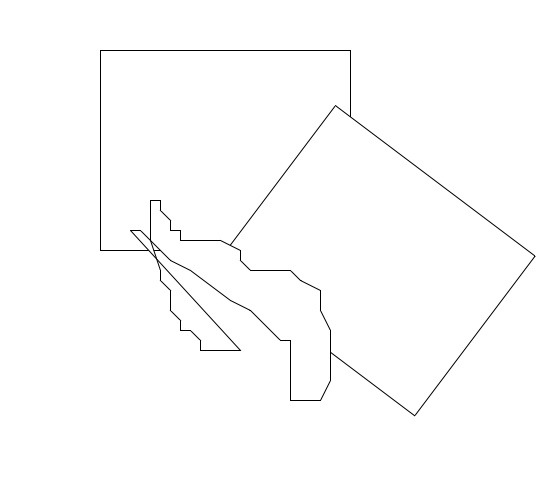
\includegraphics[width=0.45\textwidth]{figs/testImage}
  \caption{test figure}
\end{figure}
\fi
  
\section{Sets}
{\it Sets} are collections of {\it elements}. We will mostly consider sets of
numbers, but elements can be most anything.

A {\it set} can be specified by listing its elements within braces, as in
\begin{align*}
A=\{1,2,3,4,5,6\} &\ (\mbox{the possible outcomes of the roll of a die}) \\
B=\{1,2,\ldots\}  &\ (\mbox{the positive integers, commonly denoted
  $\mathbb{Z}^+$}) \\
C=\{H,T\} & (\mbox{the possible outcomes of the flip of a coin}) 
\end{align*}
We say that $5$ is an element of $A$ and denote it by $5 \in A$. Sets
are {\em unordered} collections, in other words $\{1,2,3,4,5,6\} =
\{5,2,1,3,4,6\}$. The number of times an element can appear in a set
is either 0 or 1, an element cannot appear multiple times in the set
(for that there is a different construct called {\em bags}).

Instead of listing the elements of a set, one can define a set by
specifying the precise conditions for an element to be in the set. For
example:
\begin{align*}
\mathbb{Z}^+ &= \{x: \mbox{$x$ is a positive integer}\} \\
\mathbb{R}   &= \{x: \mbox{$x$ is a real number}\} .
\end{align*}
When set $S$ is contained in set $T$ (that is, $x \in S \Rightarrow x
\in T$), we write $S \subseteq T$. For instance, $\mathbb{Z}^+
\subseteq \mathbb{R}$. The {\em empty set} contains no elements and is
denoted by $\{\}$ or $\emptyset$.

Suppose $A,B$ are two sets. The {\em intersection} of the two sets,
denoted $A\cap B$ contains the elements that are in {\em both}
sets. Thus
\begin{align*}
\{1,2,3,4,5,6\} \cap \{2,4,6,8,10\} = \{2,4,6\}
\end{align*}
The {\em union} of two sets contains those elements that are {\em
  either} $A$ or $B$ (or both), thus
\begin{align*}
\{1,2,3,4,5,6\} \cup \{2,4,6,8,10\} = \{1,2,3,4,5,6,8,10\}
\end{align*}

\subsection{Spaces and complements}
In probability we call the set of all possible outcomes (for a
particular experiment) as {\em the outcome space} and denote it by
$\Omega$. Subsets of $\Omega$ are called {\em events}. The {\em
  complement} of an event $A$ is the set of outcomes that are in
$\Omega$ but not in $A$. The complement of the set $A$ is denoted
$A^c$. For example, suppose $\Omega=\{1-10\}$ then 
\subsection{Tuples, and products of sets}

Suppose we toss a coin three times. We can represent the outcome by a 3-tuple like
$(H,H,T)$ (where $H$ means heads and $T$ means tails). The set of all
such tuples is
$$ 
\{(H,H,H), (H,H,T), (H,T,H), (H,T,T), (T,H,H), (T,H,T), (T,T,H), (T,T,T)\}.
$$
It can also be written as $\{H,T\} \times \{H,T\} \times \{H,T\}$, or even more 
simply, $\{H,T\}^3$.

More generally, if $S_1, S_2, \ldots, S_k$ are sets, then 
$S_1 \times S_2 \times \cdots \times S_k$ is the set of all $k$-tuples in which
the first entry is from $S_1$, the second entry is from $S_2$, and so on. For
instance,
\begin{align*}
\mathbb{R}^2 &= \{\mbox{all points in the plane}\} \\
\mathbb{R}^d &= \{\mbox{all points in $d$-dimensional space}\} .
\end{align*}

Note that, unlike sets, {\em order} is significant in tuples. Also
note that the same element can appear multiple times in a tuple, but
not in a set.

We are often also interested in sets of tuples that cannot be expressed as 
products of individual sets. For instance, the points in the unit circle in
$\mathbb{R}^2$ are
$$ \{(x,y): x^2 + y^2 \leq 1 \},$$
a subset of $\R^2$ that cannot be written as a product $S_1 \times S_2$.

\subsection{The size of a set}

The {\em size} of a set $A$ is the number of elements in it and is denoted
by $|A|$. Thus $|\{H,T\}|=2$, $|\emptyset|=0$ and $|\mathbb{Z}^+|=\infty$.

When $S$ is of the form 
$S_1 \times \cdots \times S_k$, then
$|S| = |S_1| \cdot |S_2| \cdots |S_k|$.

To see an example of this notation, suppose there is a group of $n$
concert-goers, each of whom is selecting a band T-shirt. The available
colors are red, yellow, and black. How many possible outcomes are
there? Well, let $C = \{\mbox{red}, \mbox{yellow}, \mbox{black}\}$ be
the set of possible colors, and represent each outcome as an $n$-tuple
in which the $i$th entry is the color of the $i$th person's T-shirt.
Then the possible outcomes are $C^n$, a set of size $|C|^n = 3^n$.

\section{Permutations and combinations}

Armed with the concepts of sets, tuples and set size we can now tackle
some more interesting combinatorial questions.

\subsection{Sampling with and without replacement when the order matters}

Suppose there are four children---Alice, Bill, Christie, and Doug---at an animal
shelter, checking out the current pool of $n$ dogs. Each child writes down the 
name of the dog he or she likes most. How many possible outcomes are there?

We can represent each outcome as a 4-tuple (Alice's choice, Bill's choice,
Christie's choice, Doug's choice) in which each entry is the name of a dog. 
So the number of outcomes is $n^4$.

Now suppose that these same children are actually picking out dogs. First Alice 
chooses a dog to adopt, then Bill chooses a dog to adopt, and so on. How many 
outcomes are there now?

In this situation, Alice has $n$ choices, but Bill has only $n-1$ choices,
Christie has $n-2$ choices, and Doug has $n-3$ choices. So there are
$n(n-1)(n-2)(n-3)$ possible outcomes.\\

The first situation is called {\it sampling with replacement}: the
outcomes are tuples in which the same element (dog) can occur more
than once. The number of such $k$-tuples, chosen from $n$ elements, is
$n^k$. In the example, $k=4$. The second situation is {\it sampling
  without replacement}: the outcomes are tuples in which no element
can be repeated. The number of such $k$-tuples, chosen from $n$
elements, is $n(n-1)(n-2) \cdots (n-k+1)$. \\

Here's a related question: how many ways are there to order (shuffle)
a deck of 52 cards?  (Each such ordering is called a {\it permutation}
of the cards.) Well, the result is a 52-tuple, drawn from a set of
size 52, in which no card is repeated. Therefore, the number of
permutations is $52 \cdot 51 \cdot 50 \cdots 1$, which is called $52$
{\em factorial} and denoted as $52!$. More generally, the number of
permutations of $n$ elements is $n$ factorial or $n!$.

Coming back to sampling $k$ out of $n$ elements without replacement,
we can write it succinctly as 
\[
n(n-1)(n-2) \cdots (n-k+1) = \frac{n!}{(n-k)!}
\]

\subsection{When the order doesn't matter}

Snow White is off to pick strawberries and asks three of the dwarfs (chosen 
from the seven: Dopey, Grumpy, Doc, Happy, Bashful, Sneezy, Sleepy) to join 
her. How many possible groups are there?

In this case, it is misleading to represent an outcome as a 3-tuple, because, 
for instance, $\mbox{(Dopey, Sleepy, Doc)}$ is a different 3-tuple from
$\mbox{(Sleepy, Dopey, Doc)}$ but they represent the same group. So if we count
tuples, we would be {\it over-counting}. Instead, we ought to represent an 
outcome as a set, $ \{\mbox{Dopey, Doc, Sleepy}\}$.

So the question becomes: how many different subsets of three dwarfs are there?
In general, a set of size $n$ has 
$${n \choose k} \ = \ \frac{n!}{k! (n-k)!} $$ 
subsets of size $k$. So in our example, the answer is ${7 \choose 3} = 35$.
\\

Let's step back and derive the main result: how many subsets of size $k$ does a
set of $n$ elements have? We can choose the subset in the following manner: first
pick one element from the set, then a second (different) element, then a third 
(different) element, and so on until we have $k$ distinct elements. This yields 
a $k$-tuple (first choice, second choice, etc), and as we saw above (sampling
without replacement when the order matters) the number of possible such tuples 
is $n(n-1) \cdots (n-k+1)$. However, we have over-counted because each subset of 
size $k$ appears multiple times amongst these $k$-tuples. To be precise, each 
subset corresponds to exactly $k!$ tuples, depending on the order in which the 
$k$ elements of the subset are chosen. Thus the number of subsets of size $k$ is
$$ \frac{n(n-1)\cdots (n-k+1)}{k!} \ = \ \frac{n!}{k!(n-k)!} .$$
\\

A second example: how many strings in $\{0,1\}^{10}$ contain exactly
{\it four} 1s?  Well, we need to choose four positions of the ten
possibilities in which to place the 1s; that is, we choose a subset of
size four from $\{1,2,\ldots,10\}$.  The number of ways to do this is
${10 \choose 4} = 210$.
\\

Let's finish with a more challenging example. You walk into a candy
store and notice that there are five types of candy. Your mother
allows you to pick exactly three pieces of candy, of whichever type(s)
you want. How many ways are there to do this?

You can represent the outcome by 5-tuple $(n_1, n_2, \ldots, n_5)$ in
which $n_i$ is the number of pieces of the $i$th type of candy. How
many such tuples are there, subject to $n_1 + n_2 + \cdots + n_5 = 3$?
To answer the question, we'll represent each tuple in a different
format, as a sequence of length 7 containing three stars and four
bars. For instance, the sequence $|\,**\,|\,|\,|\,*$ denotes
$(0,2,0,0,1)$ (two candies of type 2 and one candy of type 5): the
number of candies of type $i$ is the number of stars between the
$(i-1)$st and $i$th bars.
 
So we have rephrased the question thus: how many sequences are there
with four bars and three stars? Well, this is a sequence of size 7,
and we must pick three of the seven positions at which to place
stars. The number of such choices is ${7 \choose 3} = 35$.

       % Matematical Preliminaries 0.tex
\chapter{Probability spaces}

\section{Definition}

In order to properly understand a statement like
\begin{quote}
``the chance of getting a flush in five-card poker is about 0.2\%
(flush = all five cards are from the same suit)'',
\end{quote}
we need to specify the underlying {\it probability space}. This has two components:
\begin{enumerate}
\item A {\it sample space} or {\it space of outcomes}.

This is $\Omega = \{\mbox{all possible five-card hands}\}$.
\item The {\it probabilities of outcomes} Each outcome is assigned a
  probability, which is a non-negative real number, such that the sum
  of the probabilities over all of the outcomes is 1:
$$ \sum_{\omega \in \Omega} \pr(\omega) = 1 .$$
\end{enumerate}

In our example, assuming the cards are dealt fairly, all outcomes are equally probable, so
$$\pr(\omega) = 1/|\Omega| \mbox{\ \ \ \ \ for all $\omega \in \Omega$.} $$.

{\bf Events} are subsets of $\Omega$, in our example, the event of
interest is $A = \{\omega: \mbox{$\omega$ is a flush}\}$. This is a
subset of $\Omega$; that is, $A \subset \Omega$. Pictorially we can
represent the situation thus:

\begin{center}
%%\resizebox{1.5in}{!}{\input{figs/1.1.pstex_t}}
\end{center}

\noindent
The outer box is $\Omega$; every point in it is a particular five-card hand $\omega$. The inner set is $A$, and the probability that it occurs is
$$ \pr(A) = \sum_{\omega \in A} \pr(\omega) .$$
In general, if $\Omega$ is finite, the probability of events is the
sum of the probabilities of the outcomes in that event.\footnote{If
  $\Omega$ is continuous then this relationship does not hold and we
  need to define event probabilities differently. We will get to this
  a bit later. Till then we will only discuss finite outcome spaces,
  also referred to as ``discrete probability spaces''.}

In our example, since all outcomes are equally likely, $\pr(A) =
|A|/|\Omega|$. We now calculate this ratio.

The size of $\Omega$ is the number of 5 card hands is 
$$ |\Omega| = {52 \choose 5} = 2,598,960$$
The number of hands that are flush is the
number of suits (4) times the number of hands that can be chosen from
a single suit: 
$$|A|= 4\times {13 \choose 5} = 5,148$$ 
Thus the probability of a flush is
$$\frac{5,148}{2,598,960} \approx 0.00198$$
Which, as promised, is approximately 0.2\%.

\section{A first set of canonical examples}

\begin{enumerate}
\item {\it Roll a die.} What is the chance of getting a number $> 3$?

Probability space: sample space $\Omega = \{1,2,3,4,5,6\}$; probabilities $\pr(\omega) = 1/6$.

Event of interest: $A = \{4,5,6\}$; $\pr(A) = 1/2$.

\item {\it Roll three dice.} What is the chance their sum is 3?

The sample space is 
\begin{eqnarray*}
\Omega 
& = & \{(1,1,1), (1,1,2), \ldots, (6,6,6)\} \\
& = & \{(d_1, d_2, d_3): 1 \leq d_1, d_2, d_3 \leq 6\} \\
& = & \Omega_o \times \Omega_o \times \Omega_o 
\ \ \ = \ \ \ \Omega_o^3 \mbox{\ \ \ \ where\ } \Omega_o = \{1,2,3,4,5,6\}.
\end{eqnarray*}
The probabilities of outcomes $\omega \in \Omega$ are $\pr(\omega) = 1/6^3 = 1/216$.

The event of interest is $A = \{(1,1,1)\}$ whose probability is $\pr(A) = 1/216$.

\item {\it Roll $n$ dice.}

Sample space $\Omega = \Omega_o^n$, where $\Omega_o = \{1,2,3,4,5,6\}$. Each outcome $\omega \in \Omega$ has probability $1/|\Omega| = 1/6^n$.

\item {\it Socks in a drawer.} A drawer contains three blue socks and three red socks. You put your hand in and pick out a random sock. Then you put your hand in again and pick out another random sock. What's the chance the two of them match?

There are several ways to set up the sample space, but one possibility is to have a tuple whose first coordinate is the color of the first sock and whose second coordinate is the color of the second sock. $\Omega = \{B,R\} \times \{B,R\}$. The probabilities of outcomes are
\begin{eqnarray*}
\pr((B,B)) & = & \frac{3}{6} \cdot \frac{2}{5} \ \ = \ \ \frac{1}{5} \\
\pr((B,R)) & = & \frac{3}{6} \cdot \frac{3}{5} \ \ = \ \ \frac{3}{10} \\
\pr((R,B)) & = & \frac{3}{6} \cdot \frac{3}{5} \ \ = \ \ \frac{3}{10} \\
\pr((R,R)) & = & \frac{3}{6} \cdot \frac{2}{5} \ \ = \ \ \frac{1}{5}
\end{eqnarray*}
(Notice that they add up to 1.)

The event of interest is $A = \{(B,B), (R,R)\}$, which has probability $2/5$.

\item {\it Socks in a drawer, again.} This time the drawer has three blue socks and four red socks.

The sample space $\Omega$ is the same, but the probabilities of outcomes are different:
\begin{eqnarray*}
\pr((B,B)) & = & \frac{3}{7} \cdot \frac{2}{6} \ \ = \ \ \frac{1}{7} \\
\pr((B,R)) & = & \frac{3}{7} \cdot \frac{4}{6} \ \ = \ \ \frac{2}{7} \\
\pr((R,B)) & = & \frac{4}{7} \cdot \frac{3}{6} \ \ = \ \ \frac{2}{7} \\
\pr((R,R)) & = & \frac{4}{7} \cdot \frac{3}{6} \ \ = \ \ \frac{2}{7}
\end{eqnarray*}
The event of interest is $A = \{(B,B), (R,R)\}$, which has probability $3/7$.

\item {\it Shuffling a deck of cards.} You randomly shuffle a deck of $52$ cards and lay them out before you.

Here $\Omega = \{\mbox{all possible orderings of 52 cards}\}$. One way to compute $|\Omega|$ is to reason that there are 52 choices for what the first card in the sequence will be, 51 choices for the second card, 50 choices for the third card, and so on. Therefore
$$ |\Omega| = 52 \cdot 51 \cdot 50 \cdots 2 \cdot 1 .$$
This expression is called 52! (``52 factorial''). It is the number of {\it permutations} of 52 elements.

\end{enumerate}

\section{Tossing a fair coin}
\label{sec:FairCoin}

Suppose you toss a fair coin. The sample space is $\Omega_o = \{H,T\}$ (heads or tails), and each of the two outcomes has probability exactly $1/2$. What is more interesting is to toss the coin multiple times, independently. 

\subsection{Toss a fair coin 10 times}

Now the sample space is $\Omega = \Omega_o^{10}$; it includes, for instance, the sequence $(H,T,H,T,H,T,H,T,H,T)$. Since $|\Omega| = 2^{10} = 1024$, each element in $\Omega$ has probability exactly $1/1024$.

\begin{enumerate} 

\item What is the chance that {\it none} of the coin tosses are heads?

The event of interest is $\{(T,T,T,T,T,T,T,T,T,T)\}$, whose probability is $1/1024$.

\item What is the chance of exactly {\it one} head?

Now the event is 
$$A = \{(H,T,T,T,T,T,T,T,T,T), (T,H,T,T,T,T,T,T,T,T), \ldots, (T,T,T,T,T,T,T,T,T,H)\} .$$
Each sequence in $A$ is completely determined by the location of the $H$ within it. There are 10 possible locations; therefore $|A| = 10$, whereupon $\pr(A) = |A|/|\Omega| = 10/1024$.

\item What is the chance of exactly {\it nine} heads?

Equivalently, what is the chance of exactly one tail? This is the same calculation as before, $10/1024$.

\item What is the chance of exactly {\it two} heads?

The sequences of interest are $A = \{\omega \in \Omega: \mbox{$\omega$ has exactly 2 heads}\}$. Each such sequence is specified by the locations of its two heads; write these as a pair $(i,j)$, where $1 \leq i,j \leq 10$ and $i \neq j$. For instance, $(7,5)$ refers to $(T,T,T,T,H,T,H,T,T,T)$. 

The number of such pairs is $10 \cdot 9 = 90$ (10 choices for $i$, and thereafter just 9 choices for $j$). But this ends up double-counting sequences, because for instance, the pair $(5,7)$ also refers to $(T,T,T,T,H,T,H,T,T,T)$. Each sequence in $A$ is counted twice -- it corresponds to two pairs -- and therefore $|A| = 45$.

Finally, $\pr(A) = |A|/|\Omega| = 45/1024$.

\item What is the chance of exactly {\it four} heads?

This time, any sequence in $A = \{\omega: \mbox{has four heads}\}$ can be written as a 4-tuple $(i,j,k,l)$, where $1 \leq i,j,k,l \leq 10$ and $i \neq j \neq k \neq l$. For instance,
$(7,2,4,9)$ denotes $(T,H,T,H,T,T,H,T,H,T)$. The number of such 4-tuples is $10 \cdot 9 \cdot 8 \cdot 7 = 10!/6!$.

But once again, there is overcounting. $(7,2,4,9)$ refers to the same sequence as $(2,4,7,9)$ and $(2,7,9,4)$ and $(9,7,2,4)$ and many other 4-tuples. How many of them? The number of permutations of the four elements $2,4,7,9$, namely $4!$.

Therefore
$$ |A| = \frac{10!}{4!6!} = 210$$
and $\pr(A) = 210/1024$.

\item What is the chance of exactly {\it six} heads?

This is the same as the chance of four tails, which is identical to the previous calculation.

\end{enumerate}

In the last few calculations, we had to find the number of ways of choosing $k$ positions out of $n$ available slots (for instance, choosing 4 positions out of 10 slots where a $H$ might occur). Generalizing the argument above, the number of ways to do this is
$$ \frac{n!}{k!(n-k)!}, \mbox{\ which we write as\ } {n \choose k} $$
(pronounced ``$n$ choose $k$''). This is also called a {\it binomial coefficient}.

\subsection{Toss a fair coin $n$ times}

Now the sample space is $\Omega = \{H,T\}^n$, with each sequence of $n$ outcomes having probability exactly $1/2^n$. Let $A_k$ denote the event that the sequence has $k$ heads.

Notice that the events $A_0, A_1, \ldots, A_n$ are {\it disjoint} (if $A_i$ occurs then $A_j$ cannot occur for $j \neq i$). Moreover,
$$ \Omega = A_0 \cup A_1 \cup \cdots \cup A_n .$$
Therefore,
$$ \sum_{k=0}^n \pr(A_k) \ \ = \ \ \pr(A_0) + \pr(A_1) + \cdots + \pr(A_n) \ \ = \ \ 1 ,$$
or equivalently,
$$ \sum_{k=0}^n |A_k| \ \ = \ \ |A_0| + |A_1| + \cdots + |A_n| \ \ = \ \ |\Omega| .$$

In general, $|A_k|$ is the number of ways of placing $k$ heads in a sequence of size $n$; we've seen that this is ${n \choose k}$. And since $|\Omega| = 2^n$, the last equality tells us that
$$ \sum_{k=0}^n {n \choose k} \ \ = \ \ {n \choose 0} + {n \choose 1} + {n \choose 2} + \cdots + {n \choose n} \ \ = \ \ 2^n.$$

For example, take $n = 5$. Then
$$
|A_0| = {5 \choose 0} = 1, \  
|A_1| = {5 \choose 1} = 5, \ 
|A_2| = {5 \choose 2} = 10, \ 
|A_3| = {5 \choose 3} = 10, \ 
|A_4| = {5 \choose 4} = 5, \ 
|A_5| = {5 \choose 5} = 1
$$
and these add up to $2^5 = 32$.


\section{A second set of canonical examples}

\begin{enumerate}
\item {\it Rooks on a chessboard.} You place 8 rooks at random on a chessboard. What is the chance that they are non-attacking (that is, no rook is attacking another)?

To describe the sample space, number the squares in the chessboard as 1 through 64, and let the configuration of 8 rooks be given by a {\it set} of eight positions, $\omega \subset \{1,2,\ldots,64\}$. Thus:
$$\Omega = \{\omega \subset \{1,2,\ldots,64\}: |\omega| = 8 \} .$$
You should check that 
$$ |\Omega| \ \ = \ \ {64 \choose 8} $$
and that of these, only 8! configurations are non-attacking. 

Therefore
$$ \pr(\mbox{non-attacking configuration}) \ \ = \ \ \frac{8!8!56!}{64!} .$$

\item {\it Birthday paradox.} A room contains $n$ people. What is the chance that two of them have the same birthday?

The probability space is not properly specified, so we need to make some assumptions. First, we'll assume that the $n$ birthdays are independent (that is, a person's birthday is not influenced by anyone else's birthday). Second, we'll assume that all days are equally likely -- that is, the chance of a birthday falling on any particular day is exactly $1/365$ (we're also ignoring the issue of leap years).

Number the people $1,2,\ldots, n$, and number the days of the year $1,2,\ldots, 365$. We will represent the birthdays of the people in the room by an $n$-tuple $(\omega_1, \ldots, \omega_n)$, where $\omega_i \in \{1,2,\ldots,365\}$ is the birthday of the $i$th person. Thus $\Omega = \{1,2,\ldots, 365\}^n$ and each $\omega \in \Omega$ has probability exactly $1/365^n$.

The event of interest is
$$ A  \ \ = \ \ \{\omega: \mbox{$\omega_i = \omega_j$ for some $i \neq j$} \}.$$
This is a typical situation in which it is easier to analyze the {\it complement} of $A$ than $A$ itself (that is, it is easier to compute the probability that $A$ {\it doesn't} occur than the probability that it occurs).
$$ A^c \ \ = \ \ \Omega - A \ \ = \ \ \{\omega: \omega_1 \neq \omega_2 \neq \cdots \neq \omega_n\}.$$
In other words, $A^c$ is the event that everyone's birthday is different. What is the size of $A^c$? There are 365 choices for $\omega_1$, 364 for $\omega_2$, and so on, whereupon
$$ |A^c| \ \ = \ \ 365 \cdot 364 \cdot 363 \cdots (365-n+1) \ \ = \ \ \frac{365!}{(365-n)!}.$$Therefore
$$ \pr(A) \ \ = \ \ 1 - \pr(A^c) \ \ = \ \ 1 - \frac{365!}{(365-n)!365^n} .$$
This is exactly correct, but it is a little hard to understand intuitively. So let's do the calculation a different way, using an approximation.

A very useful fact is that for small $x$ (positive or negative), $e^x \approx 1+x$. And in fact, $e^x \geq 1+x$ no matter what $x$ is. Now let's return to the event $A^c$.
\begin{eqnarray*}
\pr(A^c) & = & \pr(\omega_2 \neq \omega_1) \cdot \pr(\omega_3 \neq \omega_1, \omega_2) \cdots \pr(\omega_n \neq \omega_1, \ldots, \omega_{n-1}) \\
& = & \left(1 - \frac{1}{365} \right) \left(1 - \frac{2}{365} \right) \cdots \left(1 - \frac{n-1}{365} \right) \\
& \leq & \exp(-1/365) \cdot \exp(-2/365) \cdots \exp(-(n-1)/365) \mbox{\ \ \ where $\exp(x)$ means $e^x$} \\
& = & \exp \left( - \frac{1}{365} \left(1 + 2 + \cdots + (n-1) \right) \right) \\
& = & \exp \left( - \frac{n(n-1)}{730} \right). 
\end{eqnarray*}
This upper bound is a very good approximation when $n$ is much smaller than $365$. 

Interestingly, when $n = 23$, we find that $\pr(A^c) \leq 0.5$, so $\pr(A) \geq 0.5$. That is, if there are 23 people in the room, chances are that two of them have the same birthday!

\item {\it Balls in bins.} You have $m$ indistinguishable balls and in front of you is a row of $n$ bins. You place each ball into a bin chosen at random.

Let's write the sample space as $\Omega = \{1,2,\ldots, m\}^n$; in each outcome $\omega = (\omega_1, \ldots, \omega_n)$, the value $\omega_i$ represents the number of balls in the $i$th bin.

Here are some interesting tidbits to prove.
\begin{itemize}
\item The chance that any particular bin is empty is at most $e^{-m/n}$.
\item If $m = 2n \ln n$, the chance that there exists an empty bin is at most $1/n$. To show this, it helps to use the {\it union bound}: for any events $A_1, \ldots, A_k$,
$$ \pr(A_1 \cup A_2 \cup \cdots \cup A_k) \ \ \leq \ \ \pr(A_1) + \pr(A_2) + \cdots + \pr(A_k).$$
\item The chance that no bin has 2 (or more) balls is at most $\exp(-m(m-1)/n)$. How is this related to the birthday paradox?
\end{itemize}
A lot of different probability spaces are simple cases of balls and bins. For instance, tossing a fair coin $m$ times is like throwing $m$ balls into $n=2$ bins (call one bin $H$ and the other bin $T$).

\section{Poker}

Poker is a family of card games wherein players make bets based on the
values of combinations of cards they possess or are shared among the
players. The eventual winner is determined by the player who survives
the betting and can form a hand with the highest value. Since making
bets requires an understanding of the potential value of a player's
hand, probability concepts can be used to make informed bets and
attempt to profit in the long run. Texas Hold'em is one of the most
popular variants of poker, and usually is the variant meant when
people say poker without specifying a particular game.

\subsection{Rules of Texas Hold'em}
In Texas Hold'em, there are five shared (or \emph{community} cards) and
two private (also known as \emph{hole} or \emph{pocket}) cards per
player. A hand consists of 5 cards in total, so at the end of the game
the value of a player's hand is determined by the highest possible
combination the player can make from the two \emph{hole} cards and the
\emph{community} cards. Each player is first dealt two cards, face
down. These cards are kept hidden until the end of the game.

Players then make bets in a clockwise circle, based on the potential
perceived value of their hand at the end of the game. When making
bets, players must \emph{call} in order to continue playing: they can
either \emph{check} the current bet, which means they must match the
highest bet previously made, or they can \emph{raise}, increasing the
value of the bet. If a player feels that their hand is not strong
enough to win, they can also \emph{fold}, or exit the game, but they
forfeit any money that they had previously bet. Bets contribute to the
\emph{pot}, the shared pool of money that the eventual winner will
claim. A round of betting continues until all players have either
\emph{checked} or \emph{folded}, i.e. the value of the bet is not
increased for one full rotation of the circle of players.

Here is a brief example of a round of betting, with hypothetical
players Alice, Bob, Carol, and Dan:
\begin{table}[h]
  \centering
  \begin{tabular}{ l || c | c | c}
    \hline
    Player & Bet & Terminology & Total value of Pot \\
    \hline
    Alice & \$2 &  & \$2 \\
    Bob & \$2 & Check & \$4 \\
    Carol & \$4 & Raise & \$8 \\
    Dan & \$4 & Check & \$12 \\
    Alice & \$4 & Check & \$14 \\
    Bob & \$2 & Fold & \$14 \\
    Carol & \$4 & Check & \$14 \\
  \end{tabular}
\end{table}
After Carol checks, everyone has either checked or folded and the
betting is over.

The initial betting is based only on the knowledge of the players' two
\emph{hole} cards. Then, the dealer deals the \emph{flop}, which are
the first three \emph{community} cards. Again, another round of
betting proceeds, with players now considering the best possible
combinations of their two \emph{hole} cards and the three cards in the
\emph{flop}, as well as the potential combinations achievable by the
last two unknown cards, and the possible combinations their opponents
may have. After the second round of betting, the dealer deals the
fourth community card, known as the \emph{turn}. Another round of
betting occurs, this time with players having knowledge of one more
card. After the third round of betting, the final community card, the
\emph{river}, is dealt. A fourth and final round of betting then takes
place, with the remaining players trying to estimate what potential
value their opponents may possess. Finally, if more than one player is
left, the \emph{showdown} occurs: players reveal the best five card
hand they can make from their \emph{hole} cards and the five
\emph{community} cards. The winner is the player who can form the
highest value hand, and takes the entire \emph{pot} as his
prize. While one cannot be sure of winning an individual game, the
goal of an intelligent poker player is to make a net profit over the
course of many games, by using the laws of probability (and
psychology) to ones advantage.

\subsection{Poker Hands}
In Texas Hold'em, hands consist of five cards. They fall under several
categories, with each category in the following list being higher than
all hands of lower categories. Within a category, hands are ordered by
the individual ranks of the cards, so for example a \emph{Flush} whose
highest card is the $10\clubsuit$ is higher ranked than a \emph{Flush}
whose highest card is the $9\heartsuit$, which is in turn higher than
any \emph{Straight}. Any leftover or unmatched cards (in the five card
hand) may be used to break ties.

\begin{enumerate}
\item Straight flush - five cards in sequence, all of the
  same suit, such as $Q\spadesuit J\spadesuit 10\spadesuit 9\spadesuit
  8\spadesuit$

\item Four of a kind - four cards of the same rank, eg. $8\spadesuit
  8\clubsuit 8\heartsuit 8\diamondsuit K\clubsuit$. In this case the
  $K\clubsuit$ would break ties.

\item Full house - three cards of one rank and two cards of another,
  eg. $6\clubsuit 6\heartsuit 6\spadesuit 9\heartsuit 9\clubsuit$.
\item Flush - five cards of the same suit, eg. $A\spadesuit
  J\spadesuit 10\spadesuit 6\spadesuit 4\spadesuit$.
\item Straight - five cards in sequence, not necessarily of the same
  suit. For example, 
\item Three of a kind - Three cards of the same rank, plus two other
  cards. For example, $10\spadesuit 10\clubsuit 10\heartsuit
  6\diamondsuit 4\diamondsuit$
\item Two pair - two pairs of cards of the same rank, plus a fifth
  card. For example, $J\clubsuit J\diamondsuit 8\spadesuit 8\clubsuit 5\heartsuit$
\item One pair - one pair of cards of the same rank, plus three
  others. For example, $K\clubsuit K\heartsuit J\spadesuit
  9\diamondsuit 4\diamondsuit$
\item High card - any hand not matching any of the above rules
  (i.e. no pairs, straights, or flushes). The value of the hand is
  determined by the value of the highest card. For example,
  $K\spadesuit J\heartsuit 8\clubsuit 7\clubsuit 4\spadesuit$

\end{enumerate}

You are dealt five cards at random from a deck of 52 cards. What is the chance of a flush? Of a straight flush? Of exactly one pair?

Let $\Omega = \{\mbox{all possible 5-card hands}\}$. Then $|\Omega| = {52 \choose 5}$ and each $\omega \in \Omega$ occurs with probability $1/|\Omega|$. 

Define three events of interest: 
\begin{eqnarray*}
F & = & \mbox{flush (all five cards of the same suit)} \\
S & = & \mbox{straight flush (same suit and consecutive)} \\
P & = & \mbox{the cards contain a single pair (eg. two 7s)}
\end{eqnarray*}

Then $|F| = 4 \cdot {13 \choose 5}$ (first choose a suit, then pick 5 cards from that suit), $|S| = 4 \cdot 10$ (first choose a suit, then choose the starting card in the sequence), and $|P| = 13 \cdot {4 \choose 2} \cdot 4^3 \cdot {12 \choose 3}$ (first choose which card occurs in the pair, then choose the two suits for that pair, then choose the suits of the remaining three cards, then choose their values).
 
\end{enumerate}

   % 1.tex - finite uniform probability
                                % spaces.
\chapter{General Probability Spaces}

In the previous chapter we showed how to calculate the probabilities
of events over finite probability spaces with discrete
distributions. In this chapter we will broaden the scope to include
non-uniform distributions, distributions over countable sets and
density distributions.

\section{Non-Uniform Distributions over Finite Sample Spaces}

Suppose we have an unfair die that is weighed in such a way that 1,2,3
have twice the probability of 4,5,6. What are these probabilities?

In our case $\Omega=\{1,2,3,4,5,6\}$ and the probability of each of
4,5,6 is half of the probability of 1, we therefor get
\[
1=\sum_{i=1}^6 P(i)=P(1)[3+\frac{3}{2}]=P(1)\frac{9}{2}
\]
so the probabilities of the different outcomes are 
\[ 
P(1)=P(2)=P(3)=\frac{2}{9},\;\; P(4)=P(5)=P(6)=\frac{1}{9}
\]

This is our first generalization of the uniform discrete
distributions studied in the previous chapter, the {\em non-uniform
  discrete distributions}

Consider another example, the wheel of chance depicted in
Figure~\ref{fig:Wheel-of-chance} part (a). Assuming that the wheel spins
smoothly the probability of each outcome is proportional to the angle
of the section corresponding to the outcome. Assuming that we measure
the angles in degrees, the probability of a section whose angle is
$\alpha$ is $\alpha/360$.

We can thus use the wheel to create any probability distribution over
a finite set of size $n$. This probability is defined by $n$ real numbers:
$p_1,p_2,\ldots,p_n$ which obey:

\begin{eqnarray}
\forall 1 \leq i \leq n: 0 \leq p_i \leq 1 \\
\sum_{i=1}^n p_i =1
\end{eqnarray}

Given these $n$ numbers we can compute the probability of any event -
any subset of the outcome space $\Omega=\{1,2,\ldots,n\}$. 
Suppose $V \subseteq \Omega$ is the event of interest, the probability
of $V$ is
\begin{equation}
P(V)=\sum_{i \in V} p_i
\end{equation}

\begin{figure}[th]
\begin{center}
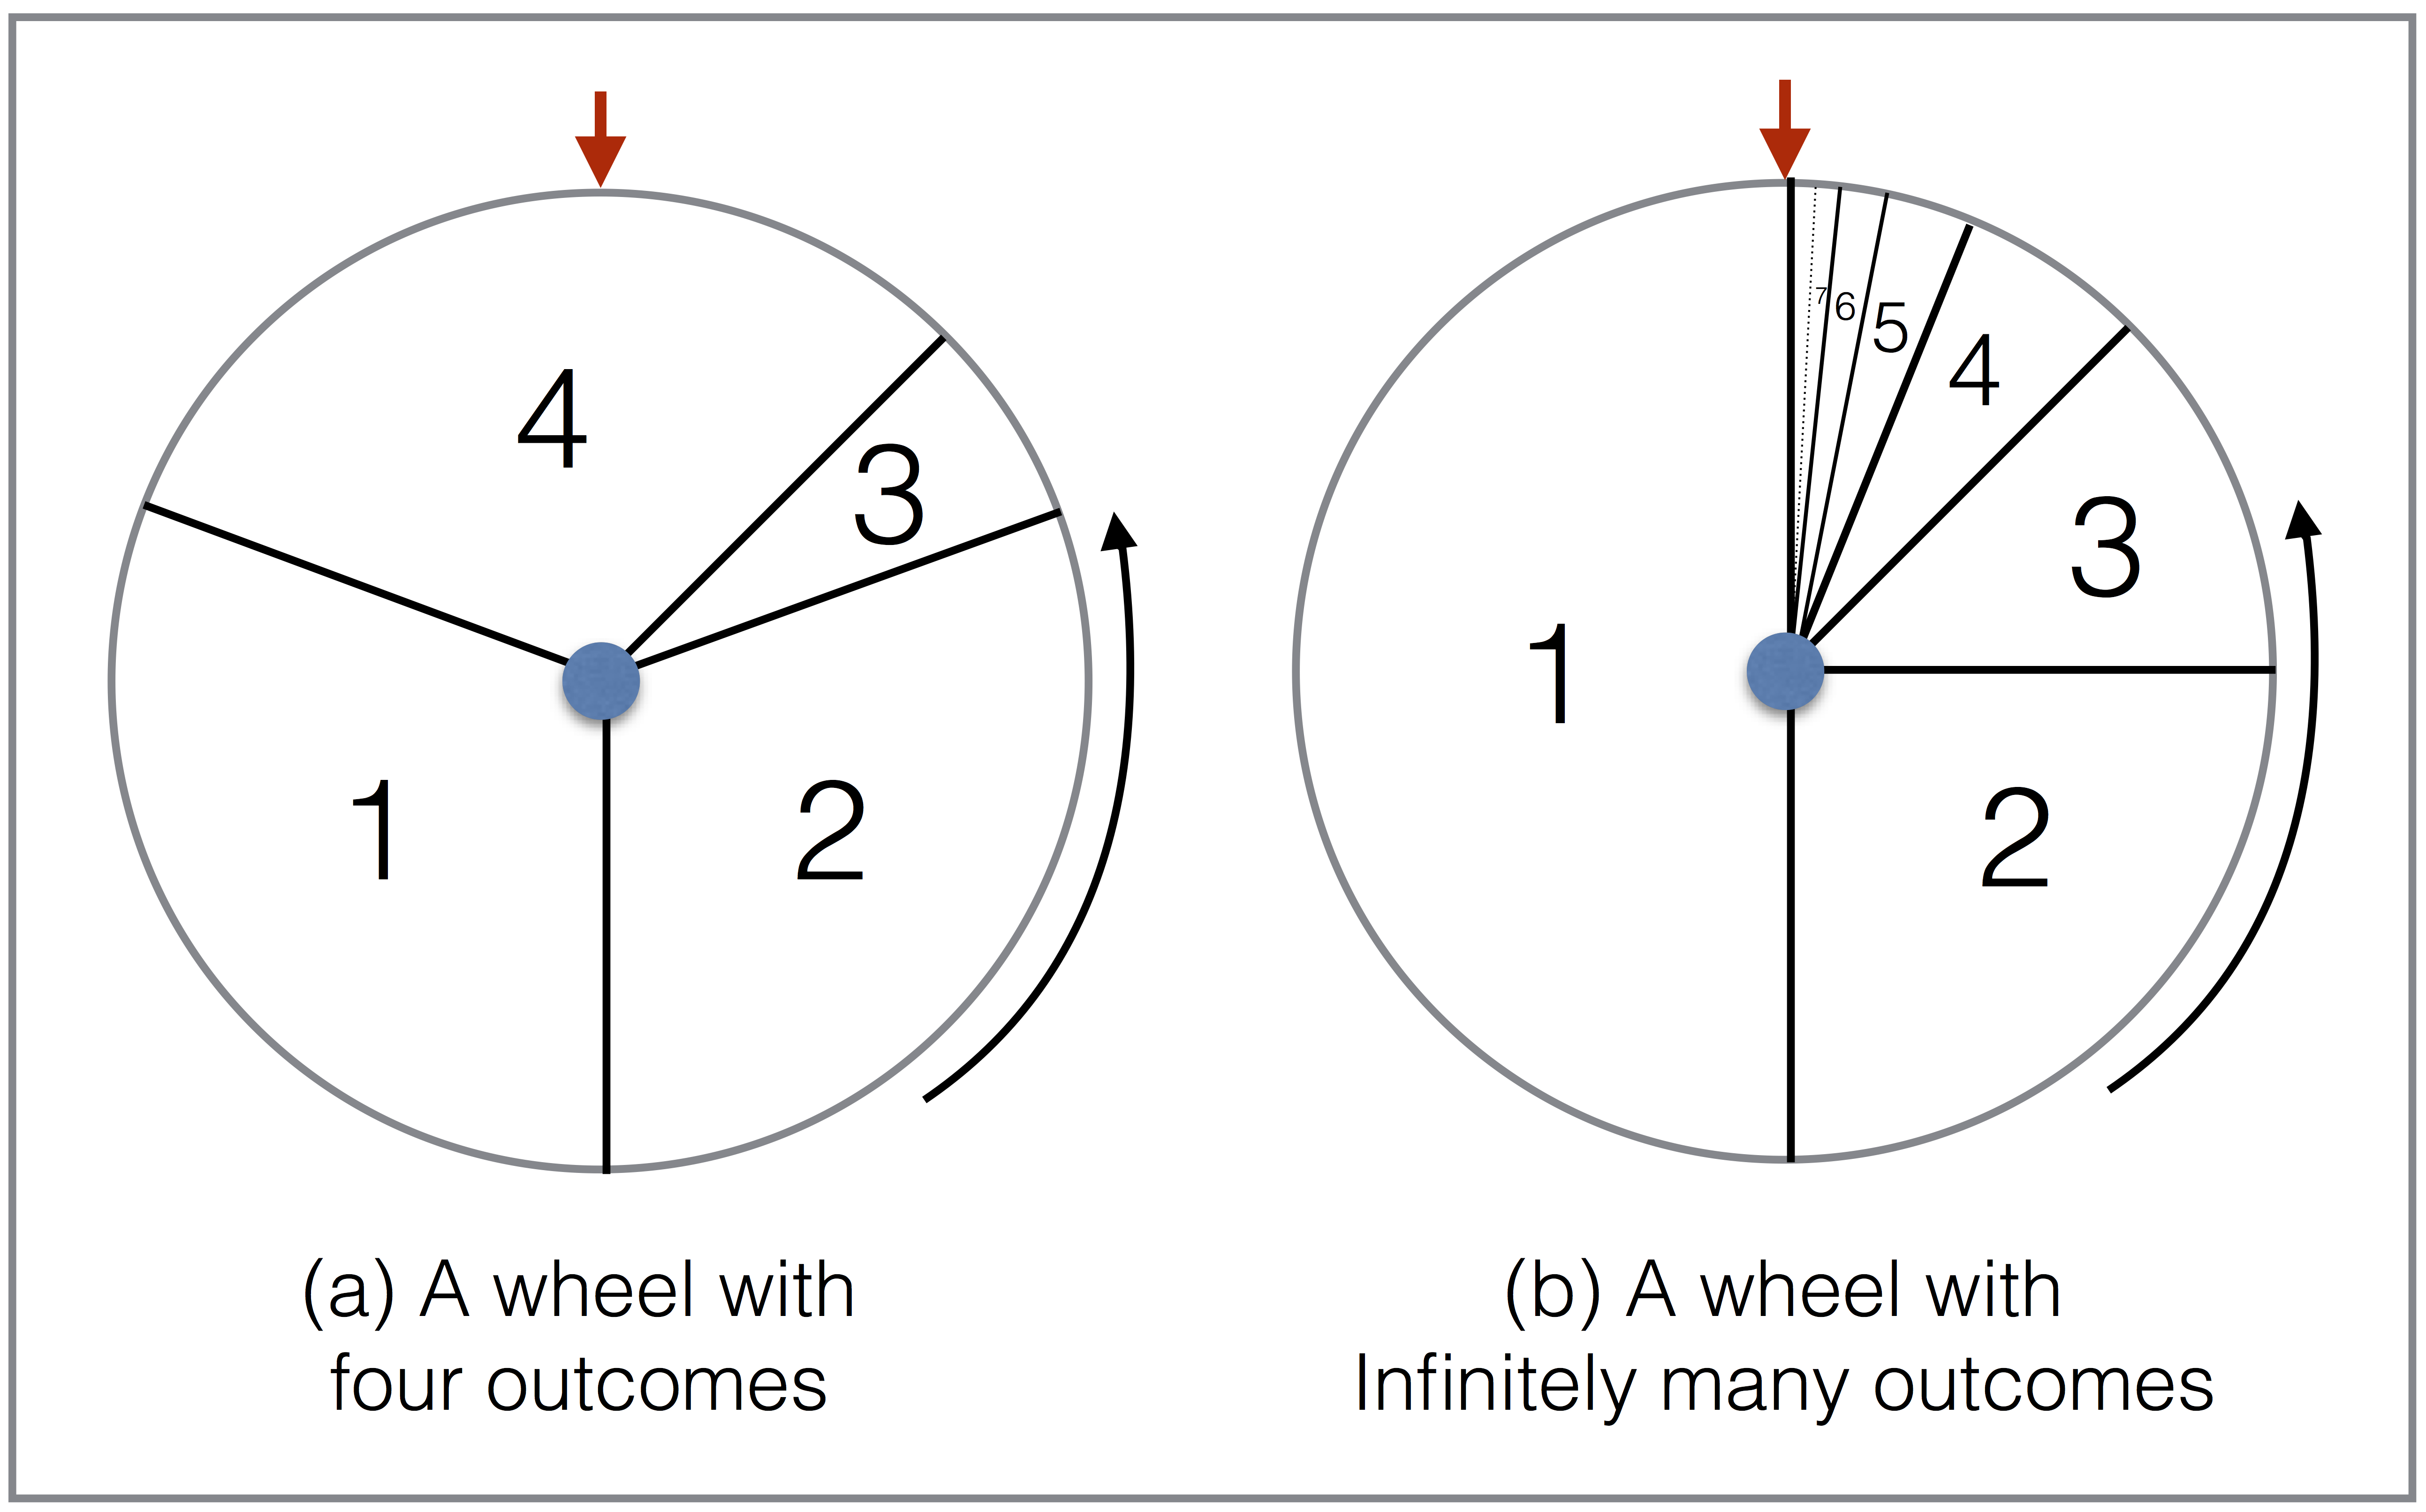
\includegraphics[width=5in]{figs/WheelsOfChanceFiniteCoutable.png}
\end{center}
\caption{Wheels of chance: the wheel is given a push and spins until
  is comes to rest. The outcome is the label of the section of the
  wheel pointed to by the red arrows. {\bf(a):} A wheel with four
  sections of different sizes. {\bf(b):} A wheel with an infinite
  number of sections, labeled with the natural numbers $1,2,3,ldots$.
\label{fig:Wheel-of-chance}}
\end{figure}

%Akshay: I'm not sure what it means to work in the rotating wheel here, since random variables and their expectations (i.e. bets) haven't yet been considered, I believe.

% Yoav: at this point the spinning wheel is just a mechanism for
% generating outcomes (elements of \Omega). The power of this
% mechanism is that it can be used to explain non-uniform discrete 
% distributions, density distributions, and even mixtures of the two.

We showed how the distribution over a finite sample space can be
specified by specifying the probability of each outcome.

What about infinite sets? Well, that depends on how ``infinite'' the set is.

As this is not a course on set theory, we will restrict our attention
to the two most useful ones, which we will describe on an intuitive
level, rather than formally. The two types of infinity that we will
consider are:
\begin{enumerate}
\item {\bf The natural numbers} The set of all natural numbers:
  $1,2,3,\ldots$ is obviously infinite. However, it is a ``small''
  type of infinite because it is {\em countable}. This means that you
  can put all of the numbers in a list.
\item{\bf The real numbers} Consider the set of points on a line, or
  even just the points on a short line segment. For example, suppose 
\[ \Omega = \left\{x | 0 \leq x \leq 1 \right\} \].
  As it turns out, the elements of this set {\em cannot} be put
  on a list, in other words, this set is not countable. As we will
  see, this means that tools from calculus are needed to define
  probability distributions on this set.
\end{enumerate}

We start with the smaller infinity, the countable infinity of the natural numbers.

\section{Distributions over the natural numbers}
Following the example of Figure~\ref{fig:Wheel-of-chance}(a) we
construct a distribution over the natural numbers using the following
iteration (depicted in part (b) of Figure~\ref{fig:Wheel-of-chance}).
\begin{enumerate}
\item The outcome 1 is given the probability $p_1=1/2$ by assigning it a
  slice that occupies $360/2 = 180$ degrees.
\item The outcome 2 is given the probability $p_2=(1/2)^2=1/4$ by
  assigning it a slice that occupies $360/4=90$ degrees. 
\item The outcome 3 is given the probability $p_3=(1/2)^3=1/8$ by
  assigning it a slice that occupies $360/8=45$ degrees.
\item ...
\item The outcome $i$ is given probability $p_i=(1/2)^i$ by assigning to
  it a slice that occupies $360/2^i$ degrees. 
\end{enumerate}

How do we know that this scheme works? In other words, how do we know
that the sum of the probabilities of all of the outcomes sums to 1?

Consider the fraction of the probability that remains after the first
$n$ outcomes have been assigned. It is not hard to convince yourself
that this remaining probability is exactly twice $p_{n+1}$ (if you
want a formal proof, try induction!):
\[
1-\sum_{i=1}^n p_i = 1-\sum_{i=1}^n (1/2)^i = (1/2)^n= 2p_{n+1}
\]
Thus each additional element halves the remaining probability. If we
repeat this for all $i$ in the natural numbers we converge, in the
limit to $1$. This is written in the following way
\[
\sum_{i=1}^{\infty} p_i = \sum_{i=1}^{\infty} (1/2)^i = 1
\]

This is our first example of a {\em convergent series} - an infinite
sequence of non-zero numbers whose sum is finite. We will use
convergent sequences later in the book, when we discuss the expected
value of a random variables. For now, we give a brief overview of
convergent and divergent sequences.

To start, the example given above is an example of a {\em geometric
  series}. The formula for the geometric series is 
\[
\sum_{i=1}^{\infty} r^i = \frac{r}{1-r}
\]
where $r$ is a real number between $0$ and $1$. 
The scheme described in the figure corresponds to $r=1/2$.

Notice that the series is infinite, but it evaluates to a finite value. 
This can happen if the sum is a geometric series. 

However, other series have this property as well. 
One that will be useful to us is the series
$$ \sum_{i=1}^\infty \frac{1}{i^2} = \frac{\pi^2}{6} $$
%(Determining the value of this series was a famous mathematical problem for decades, called the Basel problem.)
Therefore, the distribution $p_i = \frac{6}{\pi^2 i^2}$ is valid, because $ \frac{6}{\pi^2} \sum_{i=1}^\infty \frac{1}{i^2} = 1 $.

Of course, infinite series can evaluate to infinity as well. 
A well-known example we will use is the \emph{harmonic series}
$$ \sum_{i=1}^\infty \frac{1}{i} $$

\section{Tossing a biased coin}
\label{sec:BaisedCoin}

Suppose that instead of a fair coin, you have a coin whose probability of coming up heads is $p \in [0,1]$. The sample space for a single coin toss is $\Omega_o = \{H,T\}$ and the probabilities of the possible outcomes are
$$ \pr(H) = p, \ \ \pr(T) = 1-p.$$

If you toss this coin $n$ times (sample space $\Omega = \{H,T\}^n$), what is the chance of getting exactly $k$ heads? Well, pick any sequence $\omega \in \Omega$ with $k$ heads. The probability of getting precisely the outcome $\omega$ is
$$ \pr(\omega) = p^k (1-p)^{n-k} .$$
Thus the probability of $k$ heads is
$$ \mbox{(number of sequences with $k$ heads)} \cdot p^k (1-p)^{n-k} 
\ \ = \ \ 
{n \choose k} p^k (1-p)^{n-k} .$$

Sometimes we encode heads and tails numerically:
$$ \mbox{heads} \rightarrow 1, \ \ \ \mbox{tails} \rightarrow 0 .$$

In this case, a single coin flip with bias $p$ has sample space $\{0,1\}$ and is called a Bernoulli($p$) distribution. Suppose $n$ such coins are flipped, and $X_i \in \{0,1\}$ is the outcome for the $i$th coin. Then the number of heads is simply 
$$ X = X_1 + X_2 + \cdots + X_n. $$
$X$ has sample space $\{0,1,\ldots,n\}$ and is said to have a Binomial($n,p$) distribution.


\section{Density distributions}

\begin{figure}[th]
\begin{center}
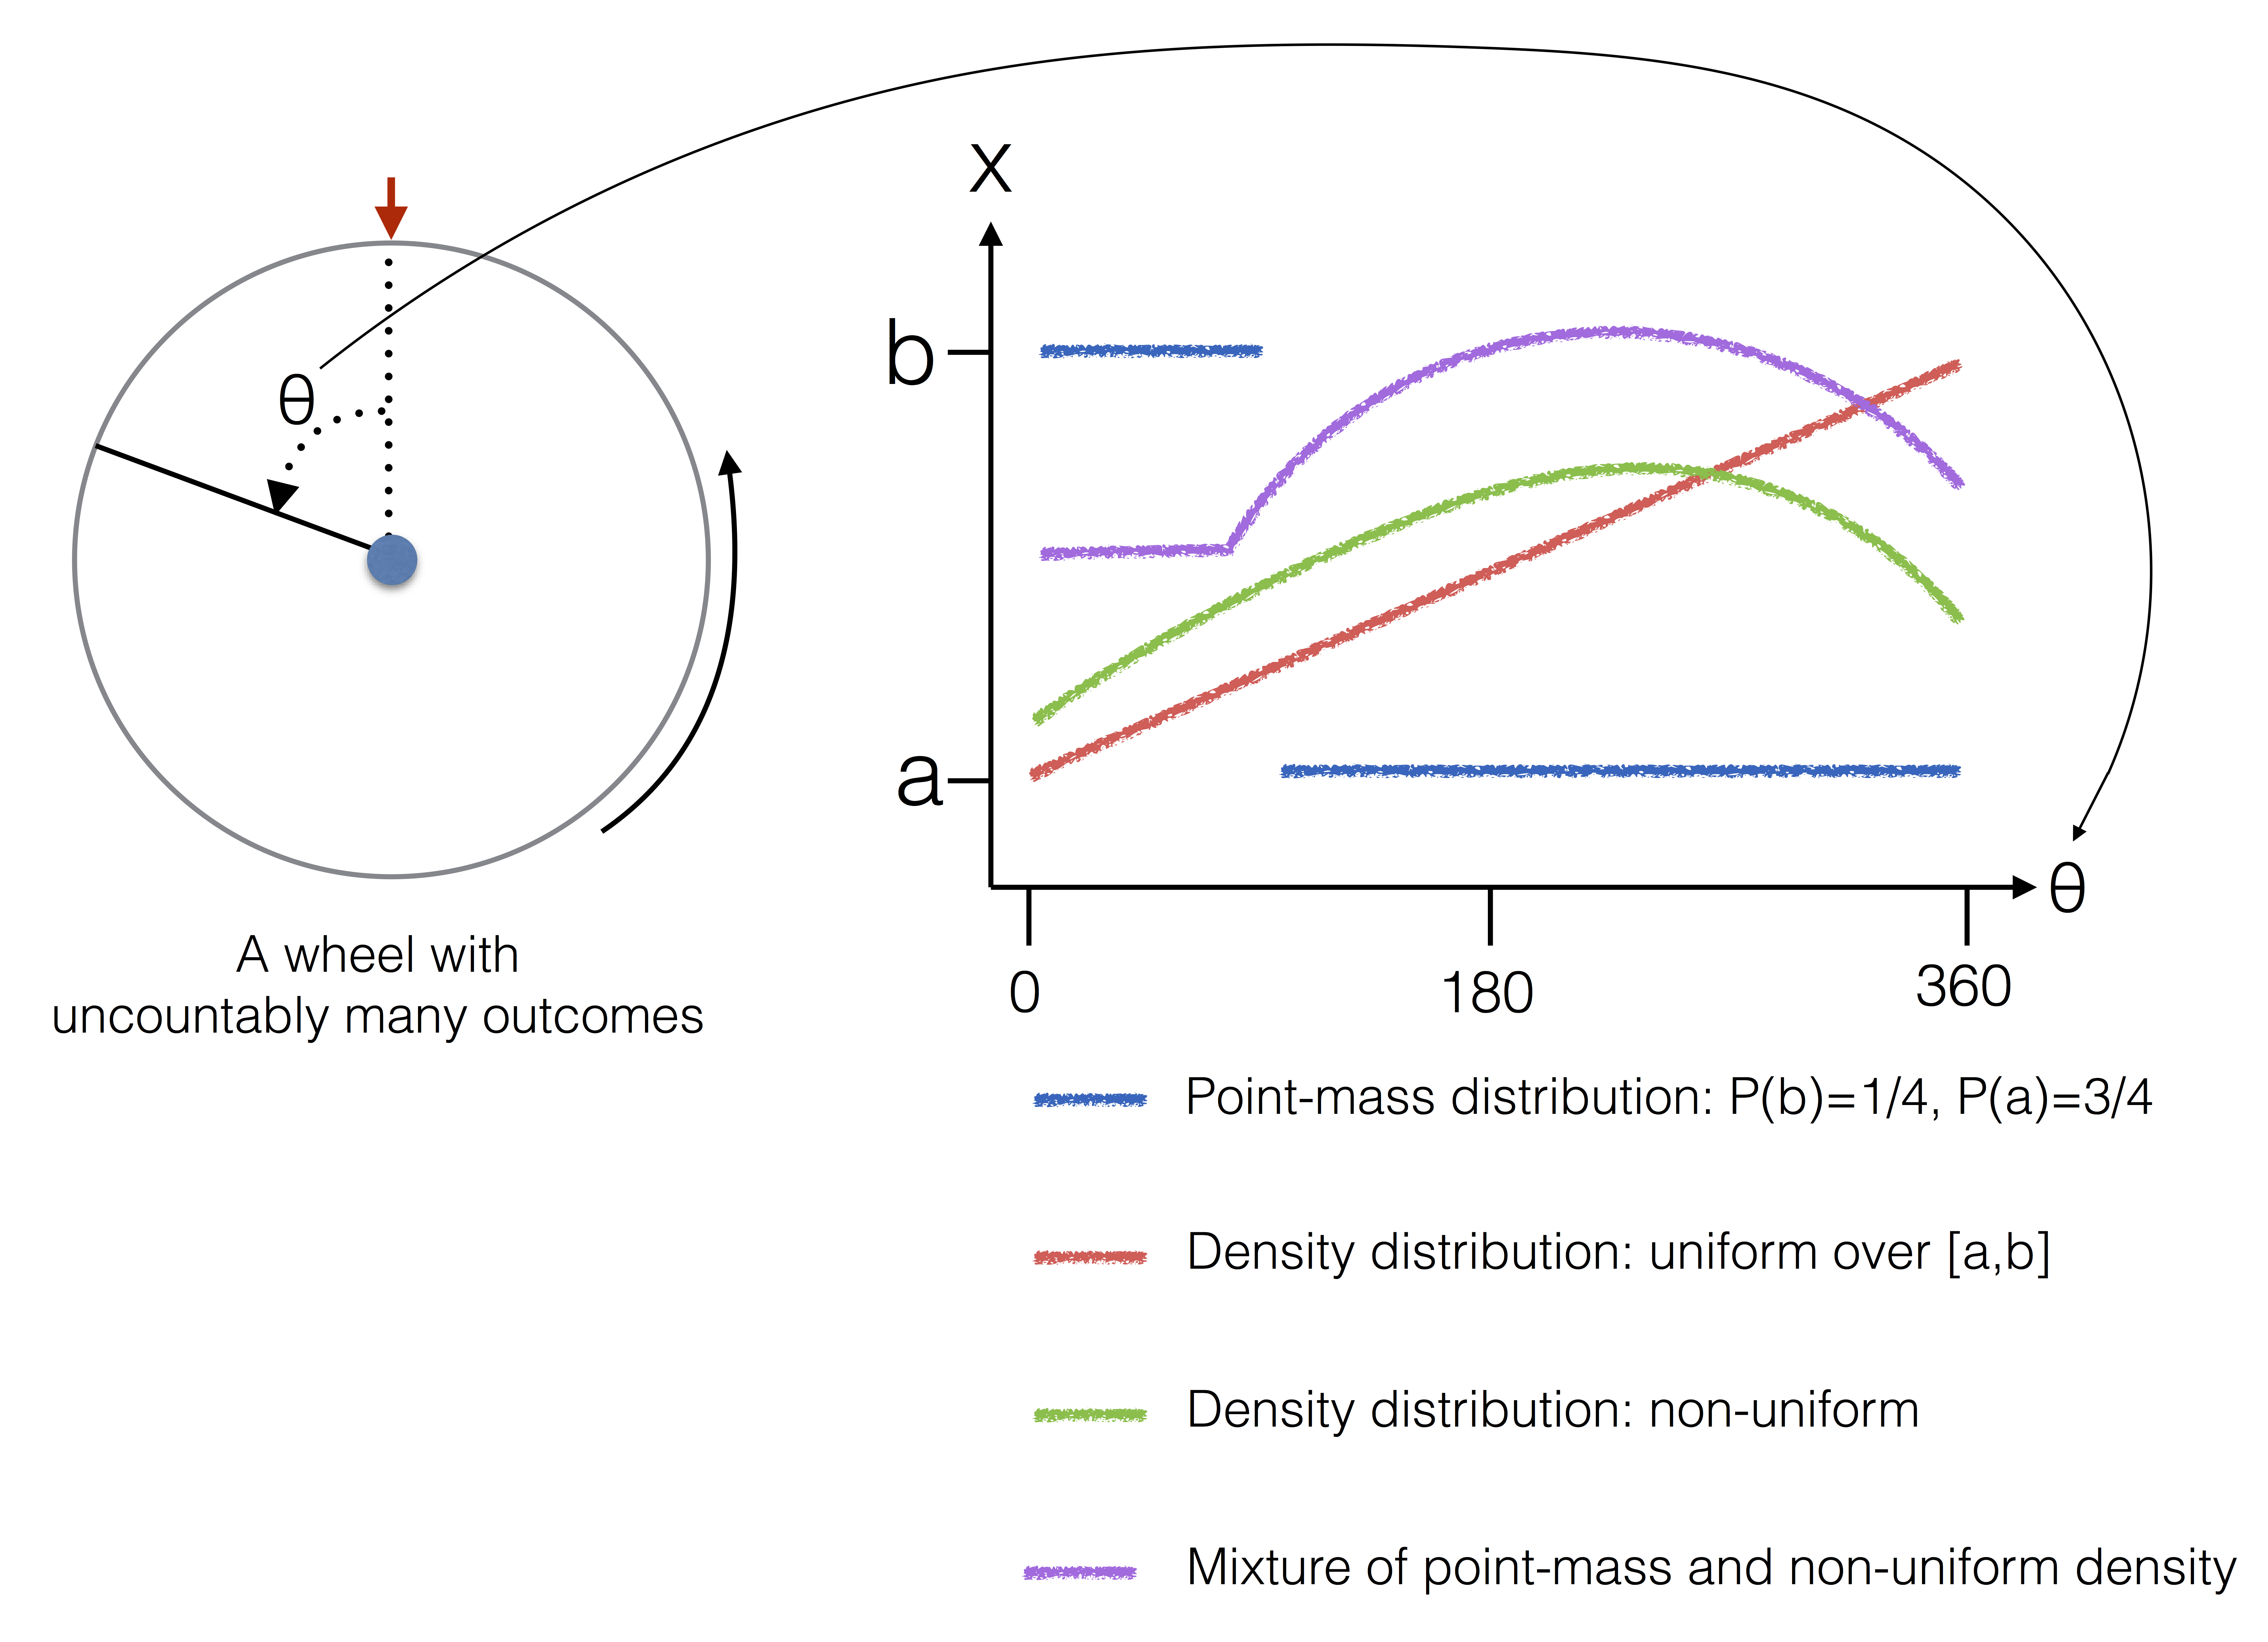
\includegraphics[width=5in]{figs/WheelsOfChanceUncountable.png}
\end{center}
\caption{{\bf Todo:} write a caption for the figure.
\label{fig:Wheel-of-chance-uncountable}}
\end{figure}

{\bf Todo: } 
\begin{itemize}
\item Kolmogorov's axioms of probability
\item Why a uniform distribution over the integers is impossible.
\item Why a uniform distribution over $[0,1]$ is possible: because
  Kolmogorov considers only countable unions.
\end{itemize}


\section{Mixture distributions}

{\bf Todo:} Describe.
\section{The limitations of histograms}

\begin{figure}[th]
\begin{center}
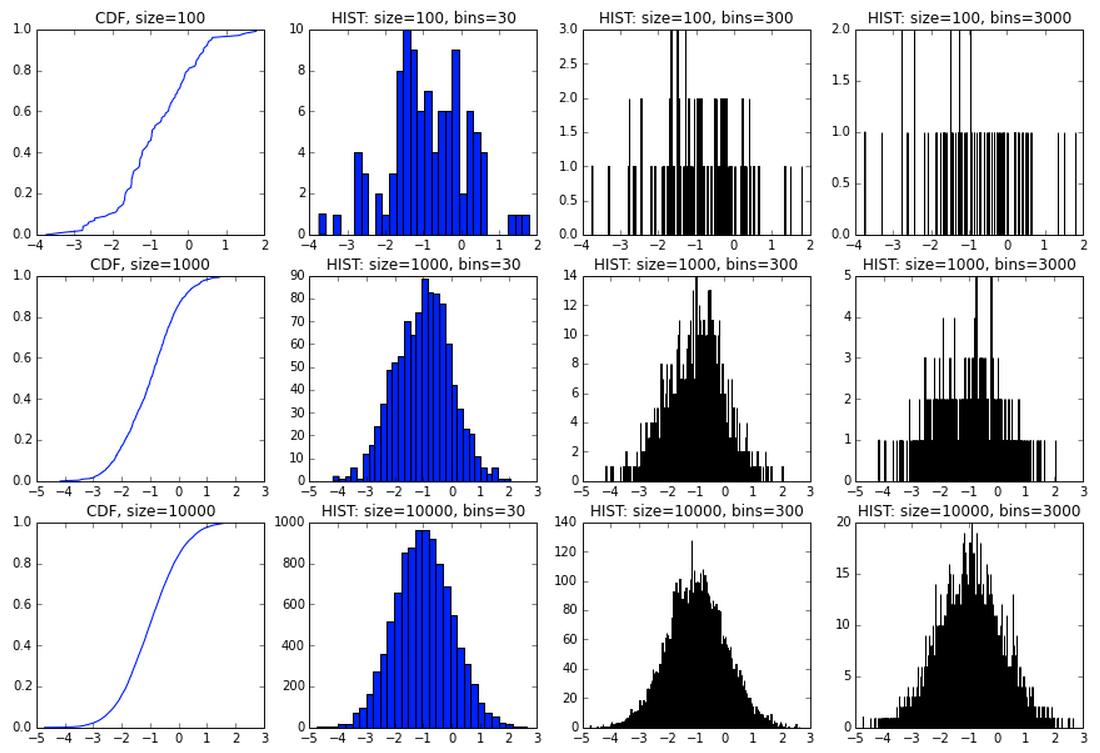
\includegraphics[width=5in]{figs/HistogramsVsCDF_D.jpg}
\end{center}
\caption{{\bf Comparison of histograms with CDF for continuous distributions:} Figure shows the effect of varying the bin width of a histogram and compares it to a CDF on the same data.\label{fig:HistogramsVsCDF_D}}
\end{figure}

\begin{figure}[th]
\begin{center}
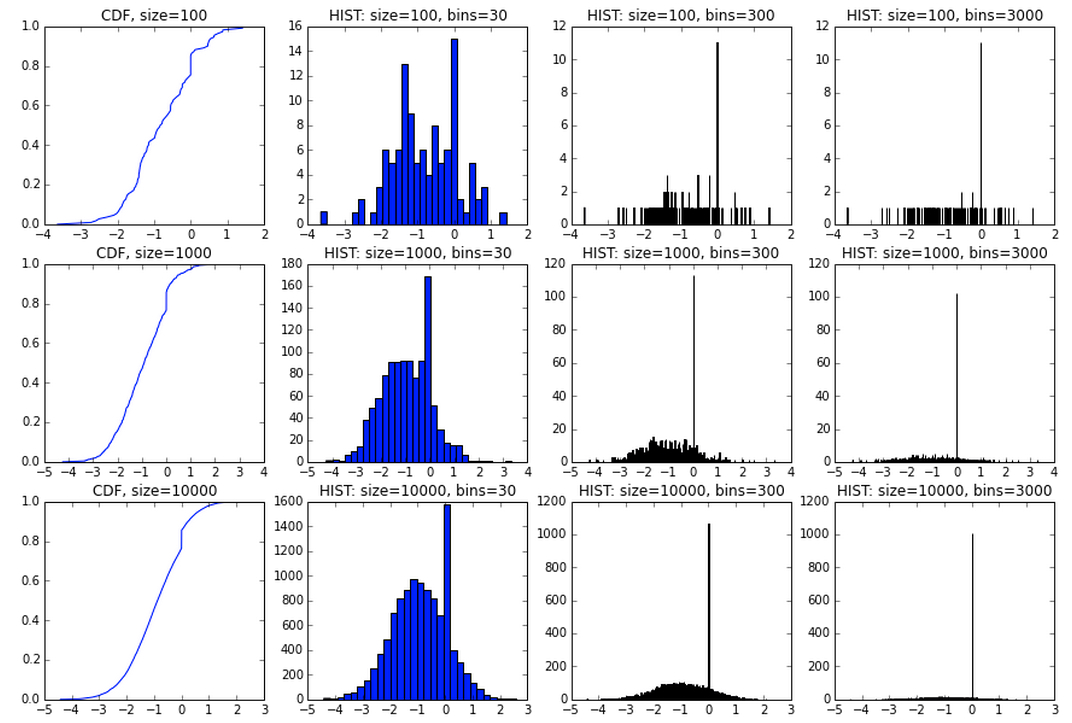
\includegraphics[width=5in]{figs/HistogramsVsCDF_PM+D.jpg}
\end{center}
\caption{{\bf Comparison of histograms with CDF for continuous distributions with a point mass:} Figure shows the effect of varying the bin width of a histogram and compares it to a CDF on the same data. \label{fig:HistogramsVsCDF_PM+D}}
\end{figure}

Figure~\ref{fig:HistogramsVsCDF_D}  and Figure~\ref{fig:HistogramsVsCDF_PM+D} show some of the limitations of using histograms.
Histograms are generated by forcing continuous data into discrete bins. While this provides an easy method to visualize the data, an incorrect choice of bin width provides little useful information.
%{\bf Todo:}Use figures to demonstrate the problems:
\begin{itemize}
\item Choosing the right width for the bins - Figure~\ref{fig:HistogramsVsCDF_D} shows the comparison between histogram and CDF for a continuous density. When there are too few bins, we lose granularity on the variation within the bin. When there are too many bins, we do not have enough data samples in each bin to accurately mirror the density. This problem is particularly accentuated when we have few samples of data. In Figure~\ref{fig:HistogramsVsCDF_D}, this scenario is shown by the histogram in the top right corner. As we move down, the number of samples increases and the histogram does a better job of representing the density. 
\item Visualizing a distribution that is a mixture of a density and a point-mass - Figure~\ref{fig:HistogramsVsCDF_PM+D} shows the challenges in the choosing the bin width when we have a distribution that is a mixture of a continuous density and a point mass. Having too many bins completely suppresses the representation of the continuous density in the histogram and accentuates the point mass. This problem is accentuated with increasing data. This scenario is represented by the histogram in the bottom right corner of Figure~\ref{fig:HistogramsVsCDF_PM+D}.
\end{itemize}
The CDF on the other hand does a better job of describing the nature of the distribution.\section{Cumulative Distribution Functions}

Our discussion so far focused on finite event spaces or event spaces
that correspond to the integers $0,1,2,\ldots$ (so-called countable
infinite sets). How do we define distributions over the real numbers?
That is an {\em uncountably} infinite set.\footnote{A set $A$ is
  uncountable if there is no one-to-one mapping from $A$ to the
  positive integers $1,2,3,4,...$. In other words, a set is
  uncountable if you cannot create a list which includes all of the
  elements in the set.}

When defining a distribution over the real it is not enough to assign
probabilities to individual points on the real line. Consider the {\em
  uniform distribution on the line segment $[0,1]$}, by which
we mean the set $\{x | 0 \leq x \leq 1\}$. We cannot assign each
point a probability larger than zero. because that would result in
$[0,1]$ an infinite probability. What we do instead is assign
probability to the line segment $0 \leq a < b \leq 1$ the probability
$b-a$. Thus for example $P([1/4,1/3])=1/3-1/4 = 1/12$.

More generally, we can define any distribution over the real line
using the {\em Cumulative Distribution Function}:
\[
\CDF(a) \doteq P(x \leq a)
\]

\begin{figure}[th]
\begin{center}
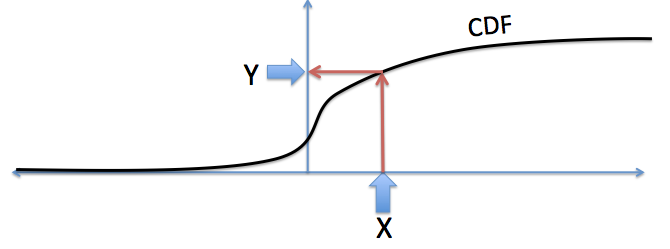
\includegraphics[width=5in]{figs/CDFmapping.png}
\end{center}
\caption{This figure depicts an example of mapping a random variable
  $X$ whose distribution is defined by a CDF (thick black curve) to
  another random variable $Y$, whose distribution is uniform in the
  interval $[0,1]$. The mapping uses the CDF as a function so that
  $Y=\CDF(X)$. \label{fig:CDFmap}}
\end{figure}

\begin{figure}[h]
\begin{center}
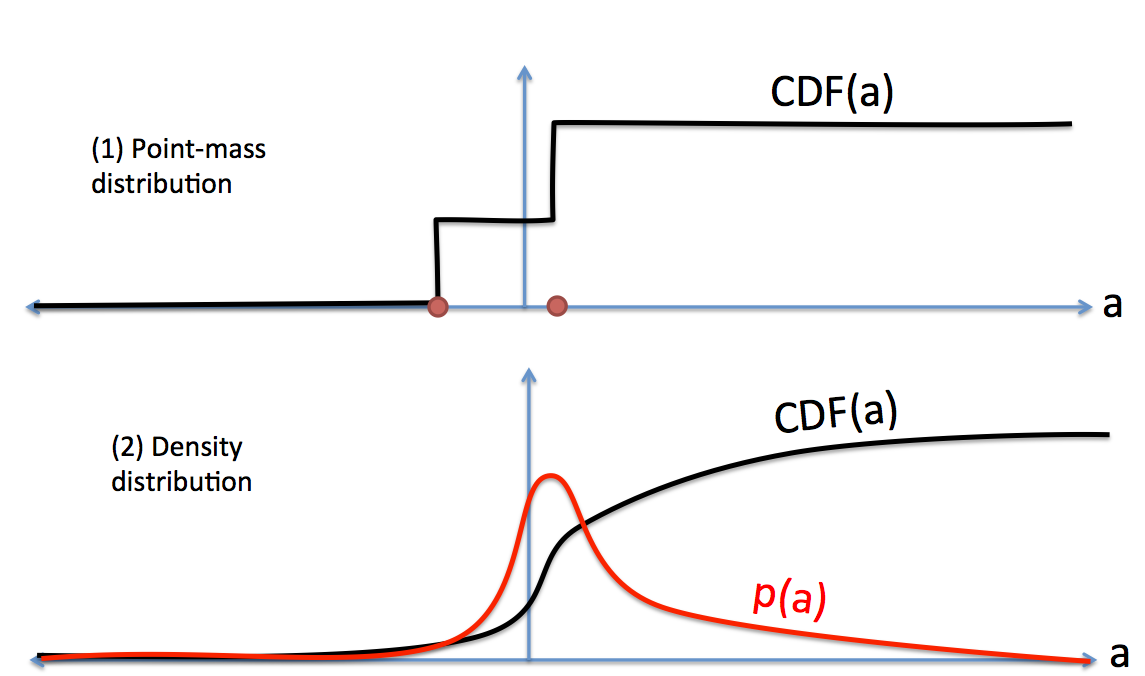
\includegraphics[width=5in]{figs/CDFs.png}
\end{center}
\caption{The CDFs for two distributions: (1) A point-mass distribution
  is a distribution that assignes non zero probabilities to two real
  values (marked by red circles) all sets that do not include at least
  one of these points have probability zero. The CDF of a point mass
  distribution is constant every where but at the point masses where
  it is discontinuous, the size of the discontinuity is the
  probability of the corresponding point. (2) A density distribution
  assigns probability zero to any single point. The CDF for such a
  distribution is a continuous increasing function that has a
  derivative. This derivative, $p(a)$ is called the {\em density function} of
  the distribution. For density distributions the CDF and the density
  function contain the same information.\label{fig:CDF}}
\end{figure}

As we see in Figure~\ref{fig:CDF} the CDF is an increasing function that
increases from zero at $-\infty$ to one at $+\infty$.

It is easy to see that $P(a<x\leq b)=\CDF(b)-\CDF(a)$.


\section{Examples of distributions on the real line}
If the distribution assigns a non-zero probability to some $x=a$ we
say that the distribution has a {\em point mass} at $a$. In that case
the $\CDF$ has a jump at $a$. We denote a point mass distribution
concentrated at the point $a$ by $PM(a)$. The distribution $PM(a)$
corresponds to a random variable such that $P(X=a)=1$.

\begin{figure}[t]
\begin{center}
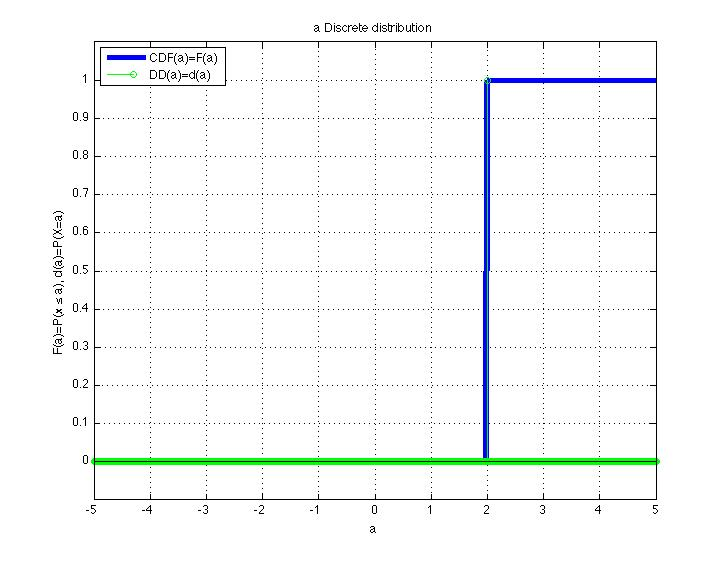
\includegraphics[width=3in]{figs/Discrete1.jpg}
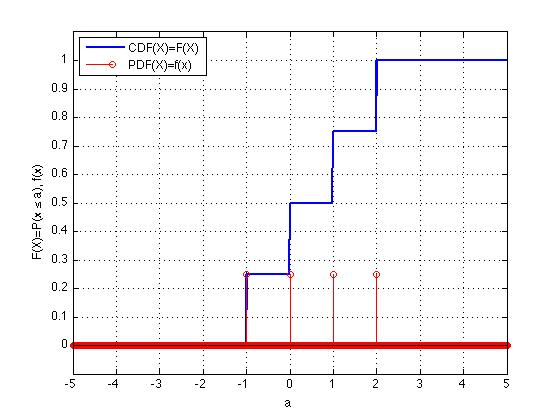
\includegraphics[width=3in]{figs/4PointMass.jpg}
\end{center}
\caption{{\bf Left:} A discrete distribution concentrated on a single
  point $P(X=2)=1$. We denote this distribution by $PM(2)$.  {\bf
    Right:} A discrete distribution distributed evenly over the four
  points $-1,0,1,2$. This distribution can be expressed as $(PM(-1)+PM(0)+PM(1)+PM(2))/4$.}
\end{figure}

\begin{figure}[b]
\begin{center}
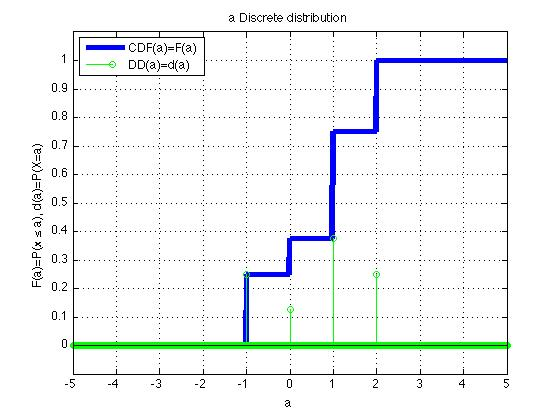
\includegraphics[width=3in]{figs/Discrete2.jpg}
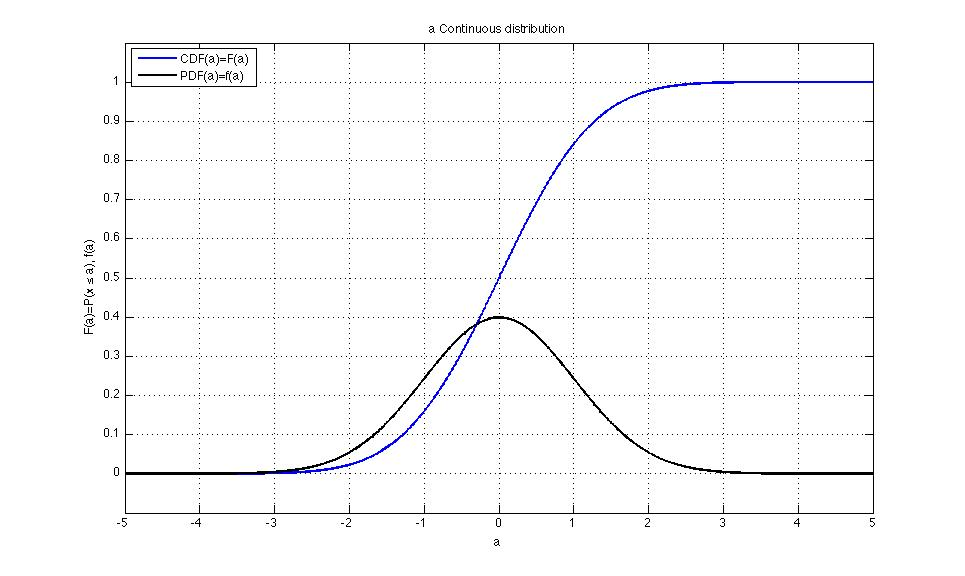
\includegraphics[width=3in]{figs/Normal.jpg}
\end{center}
\caption{{\bf Left:} A non-uniform discrete distribution. This
  distribution can be expressed as
  $(1/4)PM(-1)+(1/8)PM(0)+(5/8)PM(1)+(1/4)PM(2)$. {\bf Right:} The
  normal distribution with mean $0$ and varriance 1, denoted ${\cal
  N}(0,1)$. This is a density distribution and it's density function
is $f(x) = \frac{1}{\sqrt{2\pi}} \exp(-x^2/2)$.}
\end{figure}

\begin{figure}[t]
\begin{center}
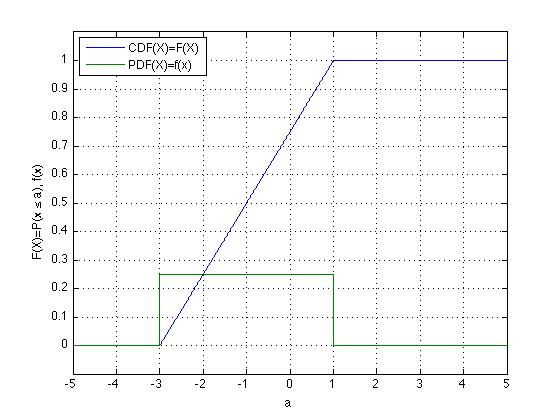
\includegraphics[width=3in]{figs/Uniform.jpg}
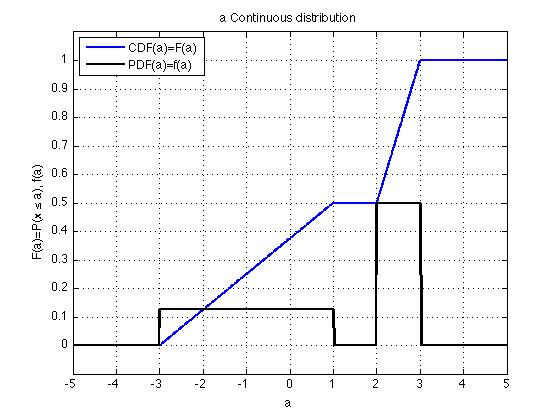
\includegraphics[width=3in]{figs/unifMixture2CDF.jpg}
\end{center}
\caption{{\bf Left:} A uniform distribution between $-3$ and $1$. We
  denote this distribution by $U(-3,1)$. {\bf Right:} A mixture of two
  uniform distributions: $(U(-3,1)+U(2,3))/2$.}
\end{figure}

\[
f(x) = \begin{cases}
0.25 & \mbox{if $ -3 \leq x \leq 1$} \\
0 & \mbox{otherwise}
\end{cases}
\]

Another important case is when the deriveative of the CDF is deifined
$p(a) = \frac{d}{dx}\left|_{x=a} \CDF(x)\right.$. The function $p(a)$
is called the {\em probability density}. Note that if $p(a)$ is
defined then, regarless of how large $p(a)$ is, $P(x=a)=0$.

When a distribution over the reals is a density distribution we can
calculate the probability of the segment $[a,b]$ using the integral:
\[
P(a < x \leq b)=\CDF(b)-\CDF(a)=\int_a^b p(x) dx
\]

\section{Throwing a dart at a dartboard} 
%{\bf todo:} Add an image of a dartboard.
\begin{figure}[H]
\begin{center}
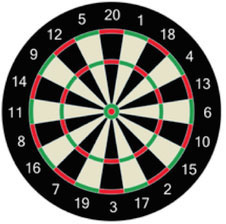
\includegraphics[width=1in]{figs/dartboard.jpg}
\end{center}
\caption{{\bf Dartboard}
 \label{fig:Dartboard}}
\end{figure}


Suppose for convenience that your dartboard has radius 1, and is
centered at the origin. Its bullseye has radius 0.1. You throw a dart
at it, which lands at a random location (all positions on the board
are equally likely). What is the chance that it lands exactly at the
origin? What is the chance that it lands in the bullseye?

This differs from earlier examples in that the sample space is infinite and continuous. It is the set of all possible locations of the dart: any point in the circle. We can represent any such point by its $(x,y)$ coordinates: $\Omega = \{(x,y): x^2 + y^2 \leq 1\}$.

The chance of landing exactly at the origin is 0, since there are infinitely many places the dart could land. It makes more sense to talk about landing in {\it regions} $A \subset \Omega$ rather than specific points $\omega \in \Omega$. In general
$$ \pr(A) = \frac{\mbox{area of $A$}}{\mbox{area of $\Omega$}} $$
and therefore $\pr(\mbox{bullseye}) = (0.1)^2 = 0.01$.

%{\bf Todo:} Use $x,y$ and $r$-the distance from the bullseye, 
%as examples of random variables.
Let $r$ denote the distance from the bullseye. The random variable $r = \sqrt{(x^2+y^2)}$. The chance of landing exactly at a distance r from the bulls eye is 0 as there are infinitely many points at a distance r from the bulls eye. These points form a circle ( denoted by C ) of radius r with the bulls eye at the center. 
From the previous result, 
$$\pr({\mbox{Landing within radius r}}) = \frac{\mbox{area of $C$}}{\mbox{area of $\Omega$}} = \Pi r^2 $$




\documentclass{report}

\usepackage[headings]{fullpage}
\usepackage{scribe}

% Packages
\usepackage{amsfonts}
\usepackage{amsmath}
\usepackage{amsthm}
%\usepackage[letterpaper,margin=1in]{geometry}
\usepackage{epsfig}
\usepackage{color}
\usepackage{array}
\usepackage{pstricks}
\usepackage{pst-plot}
%\usepackage{pstricks-add}
\usepackage{multirow}

\theoremstyle{plain}
\newtheorem{lemma}{Lemma}
\newtheorem{claim}[lemma]{Claim}
\newtheorem{theorem}[lemma]{Theorem}
\newtheorem{corollary}[lemma]{Corollary}
\newtheorem{prop}[lemma]{Property}

\theoremstyle{definition}
\newtheorem{define}[lemma]{Definition}
\newtheorem{example}[lemma]{Example}

\newtheorem{problem}{Problem}

\newcommand{\E}{\mathbb{E}}
\newcommand{\R}{\mathbb{R}}
\newcommand{\bP}{\mathbb{P}}
\newcommand{\var}{\mbox{\rm var}}
\newcommand{\pr}{\mbox{\rm Pr}}

\def\X{{\cal X}}
\def\cost{{\mbox{\rm cost}}}

\begin{document}

\course{CSE 103}
\coursetitle{Probability and statistics}
\semester{Winter 2010}
\lecturer{}
\scribe{}
\lecturenumber{2}
\lecturetopic{Multiple events, conditioning, and independence}

\maketitle

\section{Two or more events on the same sample space}

Frequently we end up dealing with multiple events $A,B,\ldots$ defined on a single sample space $\Omega$. For instance, $\Omega$ might denote the possible outcomes of picking a card from a deck, and the events of interest could include $A = \{\omega: \mbox{$\omega$ is a number}\}$, $B = \{\omega: \mbox{$\omega$ is a spade}\}$, and so on. Instead of just the single event probabilities $\pr(A)$ and $\pr(B)$, we are also interested in probabilities of combinations of events, such as $\pr(A \cap B)$ and $\pr(A \cup B)$.

\subsection{Human intuition about combined event probabilities is fallible}

Let's start with Exercise 1.2.25 from the textbook. The famous psychologists Kahneman and Tversky spent a lot of time trying to understand the nature of human rationality and decision making. For instance, do humans think probabilistically? In one experiment, they told subjects the following:
\begin{quote}
Linda is 31, single, outspoken, and very bright. She majored in philosophy in college. As a student, she was deeply concerned with racial discrimination and other social issues, and participated in anti-nuclear demonstrations.
\end{quote}
and then asked them to assess the likelihood of three events:
\begin{enumerate}
\item[(A)] Linda is active in the feminist movement.
\item[(B)] Linda is a bank teller.
\item[(C)] Linda is a bank teller who is active in the feminist movement.
\end{enumerate}
A significant majority of respondents deemed $A$ to be the most likely, followed by $C$, and lastly $B$. But $\pr(C) = \pr(A \cap B) \leq \pr(B)$! The respondents exhibited what is called a {\it conjunction fallacy}.

\subsection{Joint probability tables}

One way to write down the probabilities of pairs of events is in a table of all possible outcomes. Let's take another exercise from the textbook, 1.2.15. Here two students, John and Mary, are taking a math course in which the possible grades are $A$, $B$, and $C$. The sample space of possible outcomes can be written as $\Omega = \{A,B,C\}^2$, where the first coordinate of $\omega \in \Omega$ is John's grade and the second is Mary's grade. We can write down the probabilities of the nine possible outcomes in a $3 \times 3$ table:

\begin{center}
\begin{tabular}{|cc|ccc|} \hline
\multicolumn{2}{|c|}{} & \multicolumn{3}{c|}{Mary} \\ 
\multicolumn{2}{|c|}{} & $A$ & $B$ & $C$ \\ \hline
\multirow{3}{*}{John} & $A$ & $p_{AA}$ & $p_{AB}$ & $p_{AC}$ \\ 
                      & $B$ & $p_{BA}$ & $p_{BB}$ & $p_{BC}$ \\ 
                      & $C$ & $p_{CA}$ & $p_{CB}$ & $p_{CC}$ \\ \hline
\end{tabular} 
\end{center}

\noindent
The particular problem (see book) can be solved by writing the evidence in terms of these probabilities and adding and subtracting appropriate events.

\subsection{The union bound}

As another example, suppose that in a city,
\begin{quote}
60\% of people have a car,

20\% of people have a bicycle, and

10\% of people have a motorcycle.
\end{quote}
Anybody who lacks all three ends up walking to work, and nobody walks unless they have to. Based on this data, what fraction of people walk to work?

We don't have enough information to give an exact answer. This is because we don't know about the overlap in ownership of different vehicles: what fraction of the people with cars also have bicycles, and so on. Nonetheless, we can give upper and lower bounds. To get started, consider the experiment of picking a random person in the city, and let $\Omega$ be the space of outcomes. We then define the four events of interest: $C = \{\mbox{owns a car}\}$, $B = \{\mbox{owns a bicycle}\}$, $M = \{\mbox{owns a motorcycle}\}$, and $W = \{\mbox{walks}\}$. Since $W = \Omega - (C \cup B \cup M)$, we need to bound $\pr(C \cup B \cup M)$.

The least $\pr(C \cup B \cup M)$ could possibly be is $0.6$, which occurs when everyone who has a bicycle or motorcycle also owns a car. The most $\pr(C \cup B \cup M)$ could be is $0.9$, which happens when the sets $C,B,M$ are disjoint. Therefore $0.1 \leq \pr(W) \leq 0.4$.
 
Generalizing, we get the extremely useful {\bf union bound}: for any events $A_1, A_2, \ldots, A_k$,
$$ \pr(A_1 \cup \cdots \cup A_k) \ \leq \ \pr(A_1) + \cdots + \pr(A_k) .$$

\section{Balls in bins, or urn problems}

You have $m$ indistinguishable balls and in front of you is a row of $n$ bins. You place each ball into a bin chosen at random.

Let's write the sample space as $\Omega = \{1,2,\ldots, m\}^n$; in each outcome $\omega = (\omega_1, \ldots, \omega_n)$, the value $\omega_i$ represents the number of balls in the $i$th bin.

Here are some interesting questions one can ask.
\begin{enumerate}
\item What is the chance that the $i$th bin is empty? (What is $\pr(\omega_i = 0)$?)

Well, there are $m$ balls, and we want every single one of them to miss the $i$th bin. The probability that the first ball misses this bin is $(n-1)/n = 1 - 1/n$. The probability that the second ball misses is also $1- 1/n$, as with the third, and fourth, and so on. Therefore,
$$ \pr(\mbox{$i$th bin empty}) 
\ = \ 
\left( 1 - \frac{1}{n} \right)^m
\ \leq \ 
(e^{-1/n})^m 
\ = \ 
e^{-m/n},
$$
where we've used the formula $e^x \geq 1+x$ that we discussed earlier.

\item What is the chance that there is an empty bin if $m = n$?

Intuitively, one would expect this to be pretty close to 1 (that is, pretty much certain), because the complementary event -- no empty bins -- would occur only if every single bin received exactly one ball. Let's analyze this latter probability.
$$
\pr(\mbox{every bin gets a ball}) 
\ = \ 
\left(1 - \frac{1}{n}\right) \left( 1- \frac{2}{n}\right) \cdots \frac{1}{n} 
\ = \ 
\frac{n!}{n^n}.
$$
This is miniscule; for instance, it is less than $1/2^{n/2}$.

\item What is the chance that there is an empty bin if $m = 2n\ln n$?

When $m$ is increased from $n$ to $2n \ln n$, the chance of an empty bin drops from $\approx 1$ to $\approx 0$. To see this, let $A_i$ be the event that the $i$th bin is empty. We proved above that $\pr(A_i) \leq \exp(-m/n) = \exp(-2\ln n) = 1/n^2$. Therefore
$$
\pr(\mbox{some bin is empty}) 
\ = \ 
\pr(A_1 \cup \cdots \cup A_n) 
\ \leq \ 
\pr(A_1) + \cdots + \pr(A_n)
\ \leq \ 
n \cdot \frac{1}{n^2}
\ = \ 
\frac{1}{n}
$$
(the first inequality is the union bound). Thus with high probability (at least $1-1/n$), every bin gets at least one ball.

\item {\it The coupon collector problem.} Many probability questions turn out to be thinly disguised balls-and-bins problems. Here's an example. Suppose that each cereal box contains one of $k$ action figures (chosen uniformly at random). How many cereal boxes should you buy in order to collect all $k$ figures?

If you make the following associations:
\begin{eqnarray*}
\mbox{bin} & \equiv & \mbox{action figure} \\
\mbox{throw a ball} & = & \mbox{buy a box of cereal} \\
\mbox{every bin gets a ball} & = & \mbox{you collect all the figures},
\end{eqnarray*}
then you see that what we are really asking is, how many balls do you need to throw into $n = k$ bins in order to hit all of them? And we've already seen that $m = 2k\ln k$ balls (cereal boxes) will suffice.

\item What is the probability that some bin gets two or more balls?

This is another situation in which it is easier to study the complementary event, that every bin gets at most one ball.
$$
\pr(\mbox{every bin gets $0$ or $1$ ball})
\ = \ 
\left(1 - \frac{1}{n}\right) \left( 1- \frac{2}{n} \right)\cdots \left( 1- \frac{m-1}{n} \right)
\ = \ 
\frac{n!}{(n-m)! n^m}.
$$
Although this is exact, it is a little difficult to fathom, and so let's try an approximation instead, using $1-i/n \leq e^{-i/n}$:
\begin{eqnarray*}
\pr(\mbox{every bin gets $0$ or $1$ ball})
& = & 
\left(1 - \frac{1}{n}\right) \left( 1 - \frac{2}{n} \right) \cdots \left( 1- \frac{m-1}{n} \right) \\
& \leq & \exp(-1/n) \exp(-2/n) \cdots \exp(-(m-1)/n)  \\
& = & 
\exp\left(-\frac{1}{n} \left(1 + \cdots + (m-1) \right) \right) \\
& = &  
\exp\left(-\frac{m(m-1)}{2n} \right).
\end{eqnarray*}
This is an excellent approximation when $m \ll n$. It tells us that if $m \geq c \sqrt{n}$ (for some small constant $c$), then this probability is at most $1/2$. That is, if you throw (roughly) $\sqrt{n}$ (or more) balls into $n$ bins, then chances are that some bin will get two or more balls.

\item {\it Birthday paradox.} We saw earlier than in a room with 23 people, chances are two of them will share the same birthday.

This is yet another balls-and-bins problem:
\begin{eqnarray*}
\mbox{bin} & \equiv & \mbox{day of the year} \\
\mbox{throw a ball} & \equiv & \mbox{select birthday of a person in the room} \\
\mbox{bin with $2$ balls} & \equiv & \mbox{two people with the same birthday} .
\end{eqnarray*}
The number of bins is $n = 365$ and the number of balls is $m=23$. Using the formula we just obtained,
\begin{eqnarray*}
\pr(\mbox{two people share the same birthday})
& = & 
1 - \pr(\mbox{every bin has at most one ball}) \\
& \geq & 
1 - \exp \left(-\frac{m(m-1)}{2n} \right)
\ \ \geq \ \ 
\frac{1}{2} .
\end{eqnarray*}

\item {\it Coin tossing.}

Even the tossing of a fair coin, $m$ times, can be modeled using balls and bins. Imagine there are just $n=2$ bins (call one bin $H$ and the other bin $T$).
\end{enumerate}

\section{Conditional probability}

You meet a stranger, a random citizen of the United States. What's the chance that he (or, equally likely, she) votes for the Democratic party? Who knows, but it's probably close to $50\%$.
$$ \Omega = \{\mbox{citizens of the US}\}, \ \ E = \{\omega \in \Omega: \mbox{votes Dem}\}.$$
Now what if you find out a little bit more information: this stranger likes spicy food.
$$ F = \{\omega \in \Omega: \mbox{likes spicy food}\}.$$
How does change the odds? What is $\pr(E|F)$ (``probability of $E$ given $F$'')? Again, it's hard to say, but for illustrative purposes here is a (definitely incorrect) set of probabilities:
$$ \pr(E) = 0.5, \ \ \ \ \pr(F) = 0.2, \ \ \ \ \pr(E \cap F) = 0.15.$$
The Venn diagram for this scenario is

\begin{center}
%%\resizebox{1.5in}{!}{\input{figs/spicy.pstex_t}}
\end{center}

\noindent
If you stare at it a little bit, you will probably conclude, correctly, that $\pr(E|F)$ is the chance that a point drawn from the small blob lies inside the large blob, namely $0.15/0.2 = 0.75$. By reasoning this way, you are implicitly using {\bf the formula for conditional probability}
$$ \pr(E|F) \ = \ \frac{\pr(E \cap F)}{\pr(F)} .$$
We will make heavy use of this and of the equivalent
$$ \pr(E \cap F) = \pr(E|F) \pr(F).$$

\subsection{A few examples}

\begin{enumerate}

\item {\it Pregnancy test.} How accurate is a pregnancy test? Here we make up some numbers and compute the relevant conditional probabilities.

The sample space in this case consists of women who use the test; call this $\Omega$. There are two events on this space that we care about: $P = \{\mbox{actually pregnant}\}$ and $T = \{\mbox{test says pregnant}\}$. Suppose that the following are determined (warning: these are fabricated!):
$$ T \subset P, \ \ \ \pr(P) = 0.4, \ \ \ \pr(T) = 0.3 .$$
There are two conditional probabilities we'd like to compute.
\begin{itemize}
\item What is the chance of pregnancy if the test comes out positive?

Well, since $T \subset P$, we have $\pr(P|T) = 1.0$. Algebraically, $\pr(P \cap T) = \pr(T)$, so $\pr(P|T) = \pr(P \cap T)/\pr(T) = 1.0$.

\item What is the chance of pregnancy if the test comes out negative?

Let $T^c = \Omega - T$ be the event that the test is negative. Then $\pr(T^c) = 1 - \pr(T) = 0.7$ and $\pr(P \cap T^c) = \pr(P) - \pr(P \cap T) = 0.4 - 0.3 = 0.1$. These are the two probabilities we need.
$$ \pr(P | T^c)  \ = \ \frac{\pr(P \cap T^c)}{\pr(T^c)} \ = \ \frac{0.1}{0.7} \ \approx \ 0.14 .$$
\end{itemize}

\item {\it Rolls of a die.} You roll a die twice. What is the probability that the sum of the two rolls is $\geq 10$ if:
\begin{itemize}
\item The first roll is 6?

We could use the conditional probability formula, but that seems like overkill in so straightforward a situation.
$$ \pr(\mbox{sum $\geq 10$} \ | \ \mbox{first} = 6) 
\ = \ \pr(\mbox{second} \geq 4) \ = \ \frac{1}{2} .
$$

\item The first roll is $\geq 3$?

Okay, this is not so trivial anymore. The sample space is $\Omega = \{1,2,3,4,5,6\}^2$, with each of the 36 outcomes equally likely.
\begin{eqnarray*}
\pr(\mbox{sum $\geq 10$} \ | \ \mbox{first} \geq 3) 
& = & 
\frac{\pr(\mbox{sum $\geq 10$ {\sc and} first $\geq 3$})}{\pr(\mbox{first} \geq 3)} \\
& = &
\frac{\pr(\{(4,6), (5,5), (5,6), (6,4), (6,5), (6,6)\})}{4/6}
\ = \ 
\frac{6/36}{4/6} \ = \ \frac{1}{4} .
\end{eqnarray*}

\item The first roll is $< 6$?
\begin{eqnarray*}
\pr(\mbox{sum $\geq 10$} \ | \ \mbox{first} < 6) 
& = & 
\frac{\pr(\mbox{sum $\geq 10$ {\sc and} first $< 6$})}{\pr(\mbox{first} < 6)} \\
& = &
\frac{\pr(\{(5,5), (5,6), (4,6)\})}{5/6}
\ = \ 
\frac{3/36}{5/6} \ = \ \frac{1}{10} .
\end{eqnarray*}

\end{itemize}

\item {\it To be invisible or to fly?} A few years ago, the question was going round: ``which super power would you rather possess: the ability to make yourself invisible or to fly?'' It was perhaps an urban legend that men usually wanted to fly while women usually wanted to be invisible; and there was much speculation about the psychological reasons for this. But suppose the following statistics were obtained (warning: these numbers are fabricated!):
$$ \pr(\mbox{fly} | \mbox{male}) = 0.8, \ \ \ \pr(\mbox{invisible} | \mbox{female}) = 0.6 .$$
Then what is the overall fraction of people who would choose the ability to fly?

This cannot be answered unless it is known what fraction of the population is male and what fraction is female. Suppose it is 60-40. Then
\begin{eqnarray*}
\pr(\mbox{fly}) 
& = & \pr(\mbox{fly {\sc and} male}) + \pr(\mbox{fly {\sc and} female}) \\
& = & \pr(\mbox{fly}| \mbox{male}) \pr(\mbox{male}) + \pr(\mbox{fly}| \mbox{female}) \pr(\mbox{female}) \\
& = & (0.8)(0.6) + (0.4)(0.4) \ = \ 0.64.
\end{eqnarray*}
That is, $64\%$ would like to fly.
\end{enumerate}

\subsection{The summation rule}

In the last example, we implicitly used a {\bf summation formula}. Suppose $A_1, \ldots, A_k \subset \Omega$ are disjoint events whose union is $\Omega$ (that is, exactly one of them will occur). Then for any event $E \subset \Omega$,
$$ \pr(E) 
\ = \ 
\sum_{i=1}^k \pr(E \cap A_i) 
\ = \ 
\sum_{i=1}^k \pr(E | A_i) \pr(A_i).
$$
(If the $A_i$ are not disjoint, simply replace the first equality with a $\leq$.) We will often write $\pr(E \cap A_i)$ as $\pr(E,A_i)$.

\subsection{The Monty Hall problem}

This probability puzzle is weakly related to a game on an old TV show called {\it Let's Make a Deal}, and has been renamed after the host of that show. The host brings the game player to a room with three closed doors. One of the doors leads to a treasure chest while the other two doors each lead to a goat. The player picks a door (at random, presumably), hoping for the best. Now something interesting happens. Instead of opening that door, the host opens one of the other two doors to reveal a goat. The player is then allowed to either stick to his original guess, or to switch to the other unopened door. Which should he do?

In surveys, the majority of people feel intuitively that it doesn't make a difference. They reason that there are two unopened doors, and the treasure could be behind either of them, so each has a 50-50 chance of being the lucky door. But this is incorrect. The player should switch to the other door: by doing so, he will double his chances of getting the treasure! A conditional probability calculation shows why:
\begin{eqnarray*}
\pr(\mbox{treasure in other door}) 
& = & 
\pr(\mbox{treasure in other door} | \mbox{initial guess correct}) \pr(\mbox{initial guess correct}) + \\
& & \pr(\mbox{treasure in other door} | \mbox{initial guess wrong}) \pr(\mbox{initial guess wrong}) \\
& = & 
0 \cdot \frac{1}{3} + 1 \cdot \frac{2}{3} 
\ \ = \ \ 
\frac{2}{3} .
\end{eqnarray*}

\subsection{Another summation rule}

There is also a summation rule for conditional probabilities. Suppose $A_1, \ldots, A_k$ are disjoint events whose union is $\Omega$; and let $E,F \subset \Omega$ be any two events. Then
$$ \pr(E | F) 
\ = \ 
\sum_{i=1}^k \pr(E \cap A_i | F) 
\ = \ 
\sum_{i=1}^k \pr(E | A_i, F) \pr(A_i|F).
$$
(It's just like the regular summation rule, but operating within $F$ rather than $\Omega$.)

\subsection{Sex bias in graduate admissions}

In 1973, the dean of graduate admissions at Berkeley noticed something alarming: a male applicant had a higher chance of being admitted than a female applicant! Specifically, 
$$ \pr(\mbox{admitted} | \mbox{male}) = 0.44, 
\ \  \pr(\mbox{admitted} | \mbox{female}) = 0.35.$$
This is a significant difference given that the sample space (applicants to graduate programs at Berkeley) was very large, of size 12{,}763. The dean wondered, which departments were responsible for this bias?

To determine this, data was collected for each of the departments on campus. And it was found that no department (with a few insignificant exceptions) had any bias against females! Specifically, for each department $d$,
$$ \pr(\mbox{admitted} | \mbox{male, department $=d$}) 
\leq \pr(\mbox{admitted} | \mbox{female, department $=d$}).$$
How could this be?

Let's go back to the summation formulas for conditional probabilities.
\begin{eqnarray*}
\pr(\mbox{admit} | \mbox{male}) 
& = & 
\sum_d \pr(\mbox{admit} | \mbox{male, dept $= d$}) \pr(\mbox{dept $=d$} | \mbox{male}) \\
\pr(\mbox{admit} | \mbox{female}) 
& = & 
\sum_d \pr(\mbox{admit} | \mbox{female, dept $= d$}) \pr(\mbox{dept $=d$} | \mbox{female}) 
\end{eqnarray*}
The answer lies in the second term. Some departments (engineering) are easier to get into than others (humanities). Males tended to apply to the easier departments, while females on average applied to the harder departments. So while no individual department had bias, on the whole it looked like women had a lower probability of acceptance.

\section{Bayes' rule}

The following example is taken from {\it Probabilistic Reasoning in Intelligent Systems} by Judea Pearl:
\begin{quote}
You wake up in the middle of the night to the shrill sound of your burglar alarm. What is the chance that a burglary attempt has taken place?
\end{quote}
The relevant facts are:
\begin{itemize}
\item There is a 95\% chance that an attempted burglary attempt will trigger the alarm. That is,
$$ \pr(\mbox{alarm} | \mbox{burglary}) = 0.95 .$$
\item There is a 1\% chance of a false alarm.
$$ \pr(\mbox{alarm} | \mbox{no burglary}) = 0.01.$$
\item Based on local crime statistics, there is a one-in-10{,}000 chance that a house will be burglarized on a given night.
$$ \pr(\mbox{burglary}) = 10^{-4}.$$
\end{itemize}
We are interested in the chance of a burglary given that the alarm has sounded. We can use the conditional probability formula for this:
$$ \pr(\mbox{burglary} | \mbox{alarm}) 
\ = \ \frac{\pr(\mbox{burglary, alarm})}{\pr(\mbox{alarm})}
\ = \ \frac{\pr(\mbox{alarm} | \mbox{burglary}) \pr(\mbox{burglary})}{\pr(\mbox{alarm})}
.$$
The one term we don't immediately know is $\pr(\mbox{alarm})$. By the summation rule,
$$ 
\pr(\mbox{alarm}) 
\ = \ 
\pr(\mbox{alarm} | \mbox{burglary}) \pr(\mbox{burglary}) +
\pr(\mbox{alarm} | \mbox{no burglary}) \pr(\mbox{no burglary})
.$$
Putting it all together,
$$ \pr(\mbox{burglary} | \mbox{alarm}) 
\ = \ 
\frac{0.95 \times 10^{-4}}{0.95 \times 10^{-4} + 0.01 \times (1-10^{-4})}
\ = \ 
0.00941,
$$
about $0.94\%$. Thus our belief in a burglary has risen approximately a hundredfold from its default value of $10^{-4}$, on account of the alarm.

It is frequently the case, as in this example, that we wish to update the chances of an event $H$ based on new evidence $E$. In other words, we wish to know $\pr(H | E)$. The derivation above implicitly uses the following formula, called {\bf Bayes' rule}:
$$ \pr(H | E) 
\ = \ 
\frac{\pr(E|H) \pr(H)}{\pr(E)}.
$$  

As another example, let's look at the Three Prisoner's Paradox, which is actually just a reformulation of the Monty Hall problem. The story goes that there are three prisoners $A,B,C$ in a jail, and one of them is to be declared guilty and executed the following morning. As the night progresses, prisoner $A$ is racked with worry, and calls the prison guard over. He wants to know whether he is the unlucky one. The guard replies, ``I am not allowed to tell you whether you will be declared guilty. But I can say that prisoner $B$ will be declared innocent.'' Prisoner $A$ thinks about this for a little while and then starts worrying even more. Before he asked the question, it seemed like his chances of dying were one-in-three. But after his innocuous question, the chance seems to have risen to one-in-two!

Actually, Prisoner $A$'s chances are still one in three. The two events of interest are
\begin{eqnarray*}
G_A & = & \mbox{$A$ will be declared guilty} \\
I_B & = & \mbox{the guard, when prompted, will declare $B$ to be innocent} .
\end{eqnarray*}
Using the summation rule,
$$ 
\pr(I_B) 
\ = \ 
\pr(I_B | G_A) \pr(G_A) + \pr(I_B | G_A^c) \pr(G_A^c) 
\ = \ 
\frac{1}{2} \cdot \frac{1}{3} + \frac{1}{2} \cdot \frac{2}{3}
\ = \ 
\frac{1}{2}.
$$
Therefore, by Bayes' rule,
$$
\pr(G_A | I_B) 
\ = \ 
\frac{\pr(I_B | G_A) \pr(G_A)}{\pr(I_B)}
\ = \ 
\frac{\frac{1}{2} \cdot \frac{1}{3}}{\frac{1}{2}}
\ = \ 
\frac{1}{3}
.$$

\section{Independence}

Two events are called {\it independent} if the outcome of one (that is, whether or not it occurs) does not affect the probability that the other will occur. For instance, suppose you flip two fair coins. The outcome of either coin does not influence the other; therefore the two outcomes are independent.

Formally, we say events $A$ and $B$ (defined on some sample space $\Omega$) are independent if
$$ \pr(A \cap B) 
\ = \ 
\pr(A) \pr(B).$$
Can you show that this definition implies the following?
\begin{itemize}
\item $\pr(A | B) = \pr(A)$.
\item $\pr(B | A) = \pr(B)$.
\item $\pr(A | B^c) = \pr(A)$.
\end{itemize}

In the following examples, are events $A$ and $B$ independent or not?
\begin{enumerate}
\item You have two children. $A = \{\mbox{first child is a boy}\}$, $B = \{\mbox{second child is a girl}\}$.
\item You throw two dice. $A = \{\mbox{first is a $6$}\}$, $B = \{\mbox{sum} > 10\}$.
\item You get dealt two cards at random from a deck of 52. $A = \{\mbox{first is a heart}\}$, $B = \{\mbox{second is a club}\}$.
\item Same sample space. $A = \{\mbox{first is a heart}\}$, $B = \{\mbox{second is a $10$}\}$.
\item The three scenarios depicted in these Venn diagrams.
\end{enumerate}

\begin{center}
%%\resizebox{1.5in}{!}{\input{figs/indep1.pstex_t}}
\hskip.5in
%%\resizebox{1.5in}{!}{\input{figs/indep2.pstex_t}}
\hskip.5in
%%\resizebox{1.5in}{!}{\input{figs/indep3.pstex_t}}
\end{center}

\end{document}


\section{Tossing a biased coin}

Suppose that instead of a fair coin, you have a coin whose probability of coming up heads is $p \in [0,1]$. The sample space for a single coin toss is $\Omega_o = \{H,T\}$ and the probabilities of the possible outcomes are
$$ \pr(H) = p, \ \ \pr(T) = 1-p.$$

If you toss this coin $n$ times (sample space $\Omega = \{H,T\}^n$), what is the chance of getting exactly $k$ heads? Well, pick any sequence $\omega \in \Omega$ with $k$ heads. The probability of getting precisely the outcome $\omega$ is
$$ \pr(\omega) = p^k (1-p)^{n-k} .$$
Thus the probability of $k$ heads is
$$ \mbox{(number of sequences with $k$ heads)} \cdot p^k (1-p)^{n-k} 
\ \ = \ \ 
{n \choose k} p^k (1-p)^{n-k} .$$

Sometimes we encode heads and tails numerically:
$$ \mbox{heads} \rightarrow 1, \ \ \ \mbox{tails} \rightarrow 0 .$$

In this case, a single coin flip with bias $p$ has sample space $\{0,1\}$ and is called a Bernoulli($p$) distribution. Suppose $n$ such coins are flipped, and $X_i \in \{0,1\}$ is the outcome for the $i$th coin. Then the number of heads is simply 
$$ X = X_1 + X_2 + \cdots + X_n. $$
$X$ has sample space $\{0,1,\ldots,n\}$ and is said to have a Binomial($n,p$) distribution.
 % 2.tex
\chapter{Random variables, expectation, and variance}

\section{Random variables}

A {\it random variable} (r.v.) is defined on a probability space $(\Omega, \pr)$ and 
is a mapping from $\Omega$ to $\R$. 

The value of the random variable is fully determined by the outcome $\omega \in \Omega$.
Thus the underlying probability space (probabilities $\pr(\omega)$) induces a probability
distribution over the random variable. Let's look at some examples.

Suppose you roll a fair die. The sample space is $\Omega = \{1,2,3,4,5,6\}$, all outcomes 
being equally likely. On this space we can then define a random variable
$$ X = \left\{ \begin{array}{ll}
               1 & \mbox{if die is $\geq 3$} \\
               0 & \mbox{otherwise}
               \end{array} \right.$$
In other words, the outcomes $\omega = 1,2$ map to $X = 0$, while the outcomes 
$\omega = 3,4,5,6$ map to $X = 1$. The r.v. $X$ takes on values $\{0,1\}$, with 
probabilities $\pr(X = 0) = 1/3$ and $\pr(X=1) = 2/3$.

Or say you roll this same die $n$ times, so that the sample space is 
$\Omega = \{1,2,3,4,5,6\}^n$. Examples of random variables on this larger space are
\begin{eqnarray*}
X & = & \mbox{the number of 6's rolled,} \\
Y & = & \mbox{the number of 1's seen before the first 6.}
\end{eqnarray*}
The sample point $\omega = (1,1,1,1,\ldots,1,6)$, for instance, would map to 
$X = 1, Y = n-1$. The variable $X$ takes values in $\{0,1,2,\ldots,n\}$,
with
$$ \pr(X = k) 
\ = \ 
{n \choose k} \left(\frac{1}{6} \right)^k \left( \frac{5}{6} \right)^{n-k} $$
(do you see why?).

As a third example, suppose you throw a dart at a dartboard of radius $1$, and that it
lands at a random location on the board. Define random variable $X$ to be the distance
of the dart from the center of the board. Now $X$ takes values in $[0,1]$, and for 
any $x$ in this range, $\pr(X \leq x) = x^2$.

Henceforth, we'll follow the convention of using capital letters for r.v.'s.

\section{Finite, infinite and Undefined expectatioons}

{\bf Akshay, please put here an explanation of summable and absolutly
summable series (not necessarily using these terms).}


The simplest {\it arithmetic series} is $1,2,3,\ldots$. The sum of the first 
$n$ elements of this series is
$$ 1 + 2 + \cdots + n \ = \ \frac{n(n+1)}{2} .$$

Why? suppose that write the sum twice, first going up from $1$ to $n$
and then and then going down from $n$ down to $1$:
$$ \left(1 + 2 + \cdots + (n-1) + n\right) + 
\left(n + (n-1) + \cdots + 2 + 1\right) $$
We can rearrange the sum into a sum of $n$ pairs, the first of which
sums the first element in each list, the second sums the second
elements in each list etc:
$$ (1+n) + (2+(n-1)) + (3+(n-2)) + \cdots + (n+1) $$
It is easy to see that each pair sums to $n+1$ and that there are $n$
pairs, which gives a total of $n(n+1)$. Recalling that we summed two
copies of the original sum we get $n(n+1)/2$.

A more general arithmetic series is $a, a+s, a+2s, \ldots$
(where $a,s$ are some numbers). The sum of the first $n$ elements of this series is
$$ a + (a+s) + \cdots + (a + (n-1)s)
\ = \ 
an + s(1 + \cdots + (n-1))
\ = \ 
an + \frac{sn(n-1)}{2}.
$$
\\

One of the most common {\it geometric series} is $1, 2, 4, 8, \ldots$; the sum
of the first $n$ elements of this series is
$$ 1 + 2 + \cdots + 2^{n-1} \ = \ 2^n - 1 .$$
Another common series is $1, \frac{1}{2}, \frac{1}{4}, \ldots$,
in which the first $n$ terms sum to $2 - (1/2^{n-1})$.

More generally, a geometric series is of the form $a, ar, ar^2, ar^3, \ldots$
(where $a,r$ are some numbers), and its first $n$ terms sum to
$$ a + ar + \cdots + ar^{n-1} 
\ = \ 
\frac{a(r^n-1)}{r-1}
\ = \ 
\frac{a(1-r^n)}{1-r}.$$
The first form is more useful when $r > 1$, while the second is more useful when $r< 1$.

In the case where $|r| < 1$, we can sum the entire series (with infinitely many terms) 
to get $a/(1-r)$.

\section{The mean, or expected value}

For a random variable $X$ that takes on a finite set of possible values, the 
{\it mean}, or {\it expected value}, is
$$ \E(X) \ = \ \sum_{x} x \, \pr(X = x) $$
(where the summation is over all the possible values $x$ that $X$ can have). This
is a direct generalization of the notion of {\it average} (which is typically
defined in situations where the outcomes are equally likely). If $X$ is a continuous 
random variable, then this summation needs to be replaced by an equivalent integral; 
but we'll get to that later in the course.

Here are some examples.
\begin{enumerate}
\item {\it Coin with bias (heads probability) $p$.}

Define $X$ to be $1$ if the outcome is heads, or $0$ if it is tails. Then 
$$ \E(X) 
\ = \ 
0 \cdot \pr(X = 0) + 1 \cdot \pr(X = 1)  
\ = \ 
0 \cdot (1-p) + 1 \cdot p
\ = \ 
p .
$$

Another random variable on this space is $X^2$, which also takes on values in $\{0,1\}$.
Notice that $X^2 = X$, and in fact $X^k = X$ for all $k = 1,2,3,\ldots$! Thus, 
$\E(X^2) = p$ as well. This simple case shows that in general, $\E(X^2) \neq \E(X)^2$.

\item {\it Fair die.}

Define $X$ to be the outcome of the roll, so $X \in \{1,2,3,4,5,6\}$. Then
$$ \E(X) 
\ = \ 
1 \cdot \frac{1}{6} + 2 \cdot \frac{1}{6} + 3 \cdot \frac{1}{6} + 4 \cdot \frac{1}{6}
+ 5 \cdot \frac{1}{6} + 6 \cdot \frac{1}{6} 
\ = \ 
3.5.$$

\item {\it Two dice.}

Let $X$ be their sum, so that $X \in \{2,3,4,\ldots, 12\}$. We can calculate the probabilities
of each possible value of $X$ and tabulate them as follows:

\begin{center}
\begin{tabular}{c|c|c|c|c|c|c|c|c|c|c|c}
$x$          & 2 & 3 & 4 & 5 & 6 & 7 & 8 & 9 & 10 & 11 & 12 \\ \hline
$\pr(X = x)$ & $\frac{1}{36}$ & $\frac{2}{36}$ & $\frac{3}{36}$ & $\frac{4}{36}$ & $\frac{5}{36}$ & $\frac{6}{36}$ & $\frac{5}{36}$ & $\frac{4}{36}$ & $\frac{3}{36}$ & $\frac{2}{36}$ & $\frac{1}{36}$  
\end{tabular}
\end{center}

This gives $\E(X) = 7$.

\item {\it Roll n die; how many sixes appear?}

Let $X$ be the number of $6$'s. We've already analyzed the distribution of $X$, so
$$ E(X) 
\ = \ 
\sum_{k = 0}^n k \, \pr(X = k)
\ = \ 
\sum_{k = 0}^n k {n \choose k} \left(\frac{1}{6} \right)^k \left( \frac{5}{6} \right)^{n-k}
\ = \ 
\frac{n}{6}.
$$
The last step is somewhat mysterious; just take our word for it, and we'll get back to it later!

\item {\it Toss a fair coin forever; how many tosses to the first heads?}

Let $X \in \{1,2,\ldots\}$ be the number of tosses until you first see heads. Then
$$ \pr(X = k)
\ = \ 
\pr((T,T,T,\ldots,T,H))
\ = \ 
\frac{1}{2^k}.
$$
It follows that 
$$ \E(X) 
\ = \ 
\sum_{k=1}^\infty \frac{k}{2^k} 
\ = \ 
2.
$$
We saw in class how to do this summation. The technique was based on the formula for the
sum of a geometric series: if $|r| < 1$, then
$$ a + ar + ar^2 + \cdots \ = \ \frac{a}{1-r}.$$

\item {\it Toss a coin with bias $p$ forever; how many tosses to the first heads?}

Once again, $X \in \{1,2,\ldots\}$, but this time the distribution is different:
$$ \pr(X = k)
\ = \ 
\pr((T,T,T,\ldots,T,H))
\ = \ 
(1-p)^{k-1}p.
$$
Using the same technique as before, we get $\E(X) = 1/p$.

There's another way to derive this expectation. We always need at least one coin toss.
If we're lucky (with probability $p$), we're done; otherwise (with probability $1-p$),
we start again from scratch. Therefore $\E(X) = 1 + (1-p) \E(X)$, so that $\E(X) = 1/p$.

\item {\it Pascal's wager: does God exist?}

Here was Pascal's take on the issue of God's existence: if you believe there is
some chance $p > 0$ (no matter how small) that God exists, then you should behave
as if God exists.

Why? Well, let the random variable $X$ denote your amount of suffering.

Suppose you behave as if God exists (that is, you are good). This behavior incurs
a significant but finite amount of suffering (you are not able to do some of the
things you would like to). Say $X = 10$.

On the other hand, suppose you behave as if God doesn't exist -- that is, you 
do all the things you want to do. If God really doesn't exist, you're fine, and 
your suffering is $X = 0$. But if God exists, then you go straight to hell
and your suffering is $X = \infty$. Thus your {\it expected} suffering
if you behave badly is $\E(X) = 0 \cdot (1-p) + \infty \cdot p = \infty$.

So: to minimize your expected suffering, behave as if God exists!

\end{enumerate}


\subsection{An application to sampling}

Suppose you are interested in finding out the fraction of Americans who like sushi. 
This is some unknown value $p \in [0,1]$ that you decide to estimate by sampling.
To this end, you pick $n$ random people and poll them. Let $X_i$ be $1$ if the $i$th
person you ask likes sushi, and $0$ if not. Your estimate of $p$ is then
$$ Y \ = \ \frac{X_1 + \cdots + X_n}{n}.$$

Since $\E(X_i) = p$, it follows by linearity of expectation that
$$
\E(Y)
\ = \ 
\frac{1}{n} \left( \E(X_1) + \cdots + \E(X_n) \right)
\ = \ 
p.
$$
So $Y$ certainly has the right expected value. But how far does it typically
deviate from this expectation? Since the $X_i$ are independent, and since
each $\var(X_i) = p(1-p)$ (recall our earlier coin flip example), 
$$ 
\var(Y) 
\ = \ 
\frac{\var(X_1 + \cdots + X_n)}{n^2}
\ = \ 
\frac{\var(X_1) + \cdots + \var(X_n)}{n^2}  
\ = \ 
\frac{p(1-p)}{n}.
$$
So the standard deviation of $Y$ is $\sqrt{p(1-p)/n}$: the larger $n$ is,
the closer $Y$ stays to the desired value $p$.

\section{Linearity of expectation}

If you double each value of $X$, then you also double its average; that is, 
$\E(2X) = 2 \E(X)$. Likewise, if you raise each of its values by 1, you will
also increase the average by 1; that is, $\E(X+1) = \E(X) + 1$. More generally,
for any constants $a,b$,
$$ \E(aX + b) \ = \ a\E(X) + b.$$
Another exceptionally useful formula says that the mean value of the sum of
variables is simply the sum of their individual means. Formally, for 
any random variables $X, Y$,
$$ \E(X+Y) \ = \ \E(X) + \E(Y).$$
For example, recall our earlier example about two
rolls of a die, in which we let $X$ be the sum of the rolls and derived $\E(X)$
by first computing $\pr(X = x)$ for all $x \in \{2,3,\ldots,12\}$. Well, now
we can do it much more easily: simply write $X_1$ for the first roll and $X_2$
for the second roll, so that $X = X_1 + X_2$. We already know $\E(X_i) = 3.5$,
so $\E(X) = 7$.

More generally, for any random variables $X_1, X_2, \ldots, X_n$,
$$ \E(X_1 + \cdots + X_n) \ = \ \E(X_1) + \cdots + \E(X_n) .$$
Some quick examples:
\begin{enumerate}
\item Roll $n$ dice and let $X$ be the number of sixes. What is $\E(X)$?

This time, let $X_i$ be $1$ if the $i$th roll is a six, and $0$ otherwise. Thus 
$\E(X_i) = 1/6$, so $\E(X) = n/6$.

\item Toss $n$ coins of bias $p$ and let $X$ be the number of heads. What is $\E(X)$?

Let $X_i$ be $1$ if the $i$th coin turns up heads, and $0$ if it turns up tails. Then
$\E(X_i) = p$ and since $X = X_1 + \cdots + X_n$, we have $\E(X) = np$.

\item Toss $n$ coins of bias $p$; what is the expected number of times $HTH$ appears 
in the resulting sequence?

Let $X_i$ be $1$ if there is an occurrence of $HTH$ starting at position $i$ (so
$1 \leq i \leq n-2$). The total number of such occurrences is
$X = X_1 + X_2 + \cdots + X_{n-2}$. Since $\E(X_i) = p^2(1-p)$, we have 
$\E(X) = (n-2) p^2(1-p)$.
\end{enumerate}

\subsection{Fixed points of a permutation}

The {\it fixed points} of a permutation are the numbers that remain in their original 
position. For instance, in the permutation
$$ (1,2,3,4,5,6) \rightarrow (6,2,5,4,1,3)$$
the fixed points are 2 and 4. Let $X$ be the number of fixed points in a random 
permutation of $(1,2,\ldots, n)$; what is $\E(X)$?

Linearity is very helpful here. Define the random variable $X_i$ to be $1$ if $i$
is a fixed point, and $0$ otherwise. Then $\E(X_i) = 1/n$. Therefore
$$ \E(X) 
\ = \ 
\E(X_1 + \cdots + X_n)
\ = \ 
1.
$$
The expected number of fixed points is 1, regardless of $n$.

\subsection{Coupon collector, again}

Recall the setting: each cereal box holds one of $k$ action figures (chosen at random), and
you want to collect all the figures. What is the expected number of cereal boxes you need
to buy?

Suppose you keep buying boxes until you get all the figures. Let $X_i$ be the number of 
boxes you buy to get from $i-1$ distinct figures to $i$ distinct figures. Therefore
$X = X_1 + X_2 + \cdots + X_k$, and of course $X_1 = 1$.

What is $\E(X_i)$? Well, you already have $i-1$ of the figures, so the chance of getting
a new figure in a cereal box is $(k-(i-1))/k$. Call this $p$. Therefore, the expected amount 
of time you have to wait to get a new figure is $1/p$: just like waiting for a coin with
bias $p$ to turn up heads. That is,
$$ \E(X_i) \ = \ \frac{k}{k-i+1} .$$

Invoking linearity of expectation,
\begin{eqnarray*}
\E(X) & = & \E(X_1) + \cdots + \E(X_k) \\
      & = & \frac{k}{k} + \frac{k}{k-1} + \frac{k}{k-2} + \cdots + \frac{k}{1} \\
      & = & k \left( 1 + \frac{1}{2} + \cdots + \frac{1}{k} \right) \\
      & \approx & k \ln k.
\end{eqnarray*}
This confirms our earlier observations about the coupon collector problem: you need
to buy about $k \ln k$ boxes.

\subsection{Balls in bins, again}

Toss $m$ balls in $n$ bins; what is the expected number of {\it collisions}? Let's make
this more precise. For any $1 \leq i < j \leq m$, define the random variable $X_{ij}$ to
be $1$ if balls $i$ and $j$ land in the same bin, and $0$ otherwise. Then the
number of collisions is defined to be
$$ X  \ = \ \sum_{1 \leq i < j \leq m} X_{ij} .$$

Since $\E(X_{ij}) = 1/n$ (do you see why?), it follows that the expected number of 
collisions is 
$$ \E(X) \ = \ {m \choose 2} \frac{1}{n} \ = \ \frac{m(m-1)}{2n} .$$
So if $m < \sqrt{2n}$, the expected number of collisions is $< 1$, which means
every ball goes into a different bin. 

This relates back to the birthday paradox, where $m$ is close to the threshold $\sqrt{2n}$.

\section{Independent random variables}

Random variables $X$ and $Y$ are {\it independent} if
$$ \pr(X=x, Y=y) \ = \ \pr(X=x) \pr(Y=y) $$
for all $x,y$. In words, the joint distribution of $(X,Y)$ factors into the product
of the individual distributions. This also implies, for instance, that
$$ \pr(X = x | Y = y) \ = \ \pr(X=x) .$$

Which of the following pairs $(X,Y)$ are independent?
\begin{enumerate}
\item Pick a random card out of a standard deck. Define $X$ to be $1$ if it is a heart;
 and $0$ otherwise. Define $Y$ to be 1 if it is a jack, queen, or king; and $0$ otherwise.
\item Toss a fair coin $n$ times, and define $X$ to be the number of heads, and $Y$ to 
be $1$ if the last toss is heads (and $0$ otherwise).
\item $X$ and $Y$ take values in $\{-1,0,1\}$, and their joint distribution is given by 
the following table of probabilities.

\begin{center}
\begin{tabular}{|cc|ccc|} \hline
\multicolumn{2}{|c|}{} & \multicolumn{3}{c|}{Y} \\ 
\multicolumn{2}{|c|}{}        & $-1$   & $0$    & $1$ \\ \hline
\multirow{3}{*}{X}     & $-1$ & $0.4$  & $0.16$ & $0.24$ \\ 
                       & $0$  & $0.05$ & $0.02$ & $0.03$ \\ 
                       & $1$  & $0.05$ & $0.02$ & $0.03$ \\ \hline
\end{tabular} 
\end{center}
\end{enumerate}

If $X,Y$ are independent, they satisfy the following useful {\it product rule}:
$$ \E(XY) \ = \ \E(X) \E(Y) .$$
Another useful fact is that $f(X)$ and $g(Y)$ must also be independent, for any
functions $f$ and $g$.

\section{Variance}

If you need to summarize a probability distribution by a single number, then 
the mean is a reasonable choice -- although often the {\it median} is better 
advised (more on this later). But neither the mean nor median captures how
{\it spread out} the distribution is.

Look at the following two distributions:


\begin{center}
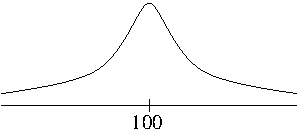
\includegraphics[width=2in]{figs/spread2.pdf}
\hskip.5in
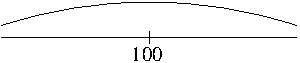
\includegraphics[width=2in]{figs/spread1.pdf}
\end{center}

\noindent
They both have the same expectation, 100, but one is concentrated near the middle 
while the other is pretty flat. To distinguish between them, we are interested
not just in the mean $\mu = \E(X)$, but also in the typical distance from the
mean, $\E(|X - \mu|)$. It turns out to be mathematically convenient to work with
the square instead: the {\it variance} of $X$ is defined to be
$$ \var(X)  \ = \ \E((X - \mu)^2) \ = \ \E((X - E(X))^2) .$$
In the above example, the distribution on the right has a higher variance that the
one on the left.

\subsection{Properties of the variance}

In what follows, take $\mu$ to be $\E(X)$.
\begin{enumerate}
\item The variance cannot be negative.

Since each individual value $(X - \mu)^2$ is $\geq 0$ (since its squared), the 
average value $\E((X - \mu)^2)$ must be $\geq 0$ as well.

\item $\var(X) = \E(X^2) - \mu^2$.

This is because
\begin{eqnarray*}
\var(X)  & = & \E((X - \mu)^2) \\
         & = & \E(X^2 + \mu^2 - 2\mu X) \\
         & = & \E(X^2) + \E(\mu^2) + \E(-2 \mu X) \ \ \mbox{(linearity)} \\
         & = & \E(X^2) + \mu^2 - 2 \mu \E(X) \\
         & = & \E(X^2) + \mu^2 - 2 \mu^2 \ = \ \E(X^2) - \mu^2.
\end{eqnarray*}

\item For any random variable $X$, it must be the case that $\E(X^2) \geq (\E(X))^2$.

This is simply because $\var(X) = \E(X^2) - (\E(X))^2 \geq 0$.

\item $\E(|X - \mu|) \leq \sqrt{\var(X)}$.

If you apply the previous property to the random variable $|X - \mu|$ instead of $X$,
you get $\E(|X - \mu|^2) \geq (\E(|X - \mu|))^2$. Therefore,
$\E(|X - \mu|) \leq \sqrt{\E(|X - \mu|^2)} = \sqrt{\var(X)}$. 
\end{enumerate}

The last property tells us that $\sqrt{\var(X)}$ is a good measure of the typical spread of
$X$: how far it typically lies from its mean. We call this the {\it standard deviation} of 
$X$.

\subsection{Examples}

\begin{enumerate}
\item Suppose you toss a coin with bias $p$, and let $X$ be $1$ if the outcome is heads, or 
$0$ if the outcome is tails.

Let's look at the distribution of $X$ and of $X^2$.

\begin{center}
\begin{tabular}{l|l|l}
Prob  & $X$ & $X^2$ \\ \hline
$p$   &  1  & 1     \\
$1-p$ &  0  & 0     
\end{tabular}
\end{center}

\noindent
From this table, $\E(X) = p$ and $\E(X^2) = p$. Thus the variance is 
$\var(X) = \E(X^2) - (\E(X))^2 = p(1-p)$.

\item Roll a 4-sided die (a tetrahedron) in which each face is equally likely to come
up, and let the outcome be $X \in \{1,2,3,4\}$.

We have two formulas for the variance: 
\begin{eqnarray*}
\var(X) & = & \E \left( (X - \mu)^2 \right) \\
\var(X) & = & \E(X^2) - \mu^2 
\end{eqnarray*}
where $\mu = \E(X)$.
Let's try both and make sure we get the same answer.
First of all, $\mu = \E(X) = (1 + 2 + 3 + 4)/4 = 2.5$. Now, let's tabulate the
distribution of $X^2$ and $(X-\mu)^2$.

\begin{center}
\begin{tabular}{l|l|l|l}
Prob  & $X$ & $X^2$ & $(X-\mu)^2$ \\ \hline
$1/4$ &  1  & 1     &  2.25 \\
$1/4$ &  2  & 4     &  0.25 \\
$1/4$ &  3  & 9     &  0.25 \\
$1/4$ &  4  & 16    &  2.25
\end{tabular}
\end{center}

\noindent
Reading from this table,
\begin{eqnarray*}
\E(X^2)     & = & \frac{1}{4} \left( 1 + 4 + 9 + 16 \right) \ \ = \ \ 7.5 \\
\E(X-\mu)^2 & = & \frac{1}{4} \left( 2.25 + 0.25 + 0.25 + 2.25 \right) \ \ = \ \ 1.25
\end{eqnarray*}
The first formula for variance gives $\var(X) = \E(X-\mu)^2 = 1.25$. The second
formula gives $\var(X) = \E(X^2) - \mu^2 = 7.5 - (2.5)^2 = 1.25$, the same thing.

\item Roll a $k$-sided die in which each face is equally likely to come up. The outcome
is $X \in \{1,2,\ldots,k\}$.

The expected outcome is
$$
\E(X) 
\ = \ 
\frac{1 + 2 + \cdots + k}{k} 
\ = \ 
\frac{\frac{1}{2} k(k+1)}{k}
\ = \ 
\frac{k+1}{2},
$$
using a special formula for the sum of the first $k$ integers. There's another for
the sum of the first $k$ squares, from which
$$
\E(X^2) 
\ = \ 
\frac{1^2 + 2^2 + \cdots + k^2}{k}
\ = \ 
\frac{\frac{1}{6}k(k+1)(2k+1)}{k}
\ = \ 
\frac{(k+1)(2k+1)}{6}.
$$
Then
$$
\var(X)
\ = \ 
\E(X^2) - (\E(X))^2
\ = \ 
\frac{(k+1)(2k+1)}{6} - \frac{(k+1)^2}{4}
\ = \ 
\frac{k^2 - 1}{12}.
$$
The standard deviation is thus approximately $k/\sqrt{12}$.

\item $X$ is the number of fixed points of a random permutation of $(1,2,\ldots,n)$.

Proceeding as before, let $X_i$ be 1 if $i$ is a fixed point of the permutation, and
0 otherwise. Then $\E(X_i) = 1/n$. For $i \neq j$, the product $X_i X_j$ is 1 only 
if both $i$ and $j$ are fixed points, which occurs with probability $1/n(n-1)$ (why?).
Thus $\E(X_i X_j) = 1/n(n-1)$. 

Since $X$ is the sum of the individual $X_i$, we have $\E(X) = 1$ and
\begin{eqnarray*}
\E(X^2) & = &
\E((X_1 + \cdots + X_n)^2) \\
& = & 
\E \left(\sum_{i=1}^n X_i^2 + \sum_{i \neq j} X_i X_j \right) \\
& = & 
\sum_i \E(X_i^2) + \sum_{i \neq j} \E(X_iX_j) \\
& = & 
n \cdot \frac{1}{n} + n(n-1) \cdot \frac{1}{n(n-1)}
\ = \ 
2.
\end{eqnarray*}
Thus $\var(X) = \E(X^2) - (\E(X)^2) = 1$. This means that the number of fixed points
has mean 1 and variance 1: in short, it is quite unlikely to be very much larger than
1.
\end{enumerate}

\subsection{Another property of the variance}

Here's a cartoon picture of a well-behaved distribution with mean $\mu$ and 
standard deviation $\sigma$ (that is, $\mu = \E(X)$ and $\sigma^2 = \var(X)$).

\begin{center}
%%\resizebox{2in}{!}{\input{figs/var.pstex_t}}
\end{center}

\noindent
The standard deviation quantifies the {\it spread} of the distribution
whereas the mean specifies its {\it location}. If you increase all values of
$X$ by 10, then the distribution will shift to the right and the mean will 
increase by 10. But the spread of the distribution -- and thus the standard
deviation -- will remain unchanged.

On the other hand, if you double all values of $X$, then its distribution 
becomes twice as wide, and thus its standard deviation $\sigma$ is doubled. 
Which means that its variance, which is the square of the standard deviation,
gets multiplied by 4.

In summary, for any constants $a,b$:
$$ \var(aX+b) = a^2 \var(X) .$$
Contrast this with the mean: $\E(aX + b) = a \E(X) + b$.

\subsection{Linearity of variance}

If $X$ and $Y$ are independent random variables, then $\var(X+Y) = \var(X) + \var(Y)$.
More generally, if $X_1, \ldots, X_n$ are independent, then
$$ \var(X_1 + \cdots + X_n)
\ = \ 
\var(X_1) + \cdots + \var(X_n).
$$
In contrast, linearity of expectation ($\E(X+Y) = \E(X) + \E(Y)$) holds
even if the random variables are {\it not} independent.


 % 3.tex
\chapter{Covariance, correlation and dependence}

Two random variables $X,Y$ are independent if and only if for any
constants $a,b$
we have:
\[
P(X\leq a \text{ and } Y \leq b)=P(X\leq a)P(Y \leq b)
\]
If $X,Y$ are restricted to the integers, then they are independent if
and only if for any two integers $i,j$
\begin{equation} \label{eqn:independentRVs}
P(X=i \text{ and } Y=j)=P(X=i)P(Y=j)
\end{equation}
Suppose we further restrict $X,Y$ to the integers $1,\ldots,100$. In
order to check whether or not $X$ and $Y$ are dependent we need to
check $100^2=10000$ conditions. Checking for independence of these random
variables requires estimating 10,000 joint probabilities, which in
turn requires very large samples.

There is an easy to calculate stand-in for dependence, called
the {\em covariance}, which we will now describe. If the covariance is not
zero then the two random variables are dependent. However, a
covariance of zero between two random variables {\em does not} imply
that they are independent.

The covariance of $X$ and $Y$ is defined as
\[
Cov(X,Y) = E\left[ (X-E(X))(Y-E(Y)) \right]
\]
Note that $Cov(X,X)=Var(X)$. We can simplify the expression for the
covariance as follows:
\[
E\left[ (X-E(X))(Y-E(Y)) \right]
=E[XY]-E[E[X]Y]-E[XE[Y]]+E[X]E[Y]
=E[XY] -E[X]E[Y]
\]
We will now show that if $X$ and $Y$ are independent then the
covariance is zero. We will show this for integer valued random
variables~\footnote{The extension to continuous random variables is
  straight forward, but involves some technical issues involving
  integration that we will not get into here.}
\begin{eqnarray}
E[XY]&=&\sum_{i,j} ij P(X=i \text{ and } Y=j) \label{EXY:1}\\ 
&=& \sum_{i,j} ij P(X=i)P(Y=j) \label{EXY:2}\\
&=& \left( \sum_i i P(X=i) \right)\left( \sum_j j P(Y=j) \right)\label{EXY:3}\\
&=&E[X]E[Y] \label{EXY:4}
\end{eqnarray}
Equation~(\ref{EXY:1}) follows from the definition of expectation
($i,j$ vary from $-\infty$ to $+\infty$). Equation~(\ref{EXY:2})
follows from Equation~(\ref{eqn:independentRVs}). We separate the
double summation in Equation~(\ref{EXY:2}) into a product of two sums
to get Equation~(\ref{EXY:3}), and finally use the definition of
expectation to get Equation~(\ref{EXY:4}). Thus we have shown that
when two random variables $X,Y$ are independent, then $E[XY]=E[X]E[Y]$
and thus $Cov(X,Y)=E[XY]-E[X]E[Y]=0$.

Intuitively, $Cov(X,Y)>0$ indicates that when $X$ is large $Y$ also
tends to be large. When this happens we say that $X$ and $Y$ are {\em
  correlated}. If $Cov(X,Y)<0$ we say that $X$ and $Y$ are {\em
  anti-correlated}, and if $Cov(X,Y)=0$. We say that $X$ and $Y$ are
{\em uncorrelated}. 

One problem with the covariance is it's sensitivity to the units in
which the random variables are measured, changing the scale changes
the covariance. Suppose the sample space corresponds to people and
suppose we consider two random variables for each person: $H$ is the
height of the person, in inches, and $W$ is the weight of the person,
in pounds.  We expect the the $H$ and $W$ are correlated. However, how
should we measure the {\em degree} of correlation? $Cov(H,W)$ will
decrease if we decide to use feet instead of inches because that would 
decrease each height by a factor of 12 and we get
$Cov(H/12,W)=Cov(H,W)/12$. In order to remove the effect of scale we
use a normalized version of the covariance, called the correlation
coefficient:
\[
Corr(X,Y) \doteq \frac{Cov(X,Y)}{\sqrt{Var(X)Var(Y)}}
\]
The correlation coefficient is a number in the range $[-1,1]$. As with
the Covariance, if $Corr(X,Y)>0$ we say that $X$ and $Y$ are {\em
  correlated}, if $Corr(X,Y)=0$ we say that $X$ and $Y$ are {\em
  uncorrelated} and if $Corr(X,Y)<0$ we say that $X$ and $Y$ are {\em
  anti-correlated}.

The extreme cases are interesting. If $Corr(X,Y)=1$ it means that
$X=aY$ for some $a>0$ while if $Corr(X,Y)=-1$, $X=aY$ for some
$a<0$. These and other interesting cases are depicted in Figure~\ref{fig:corrCoeff}.

\begin{figure}[tb]
\begin{center}
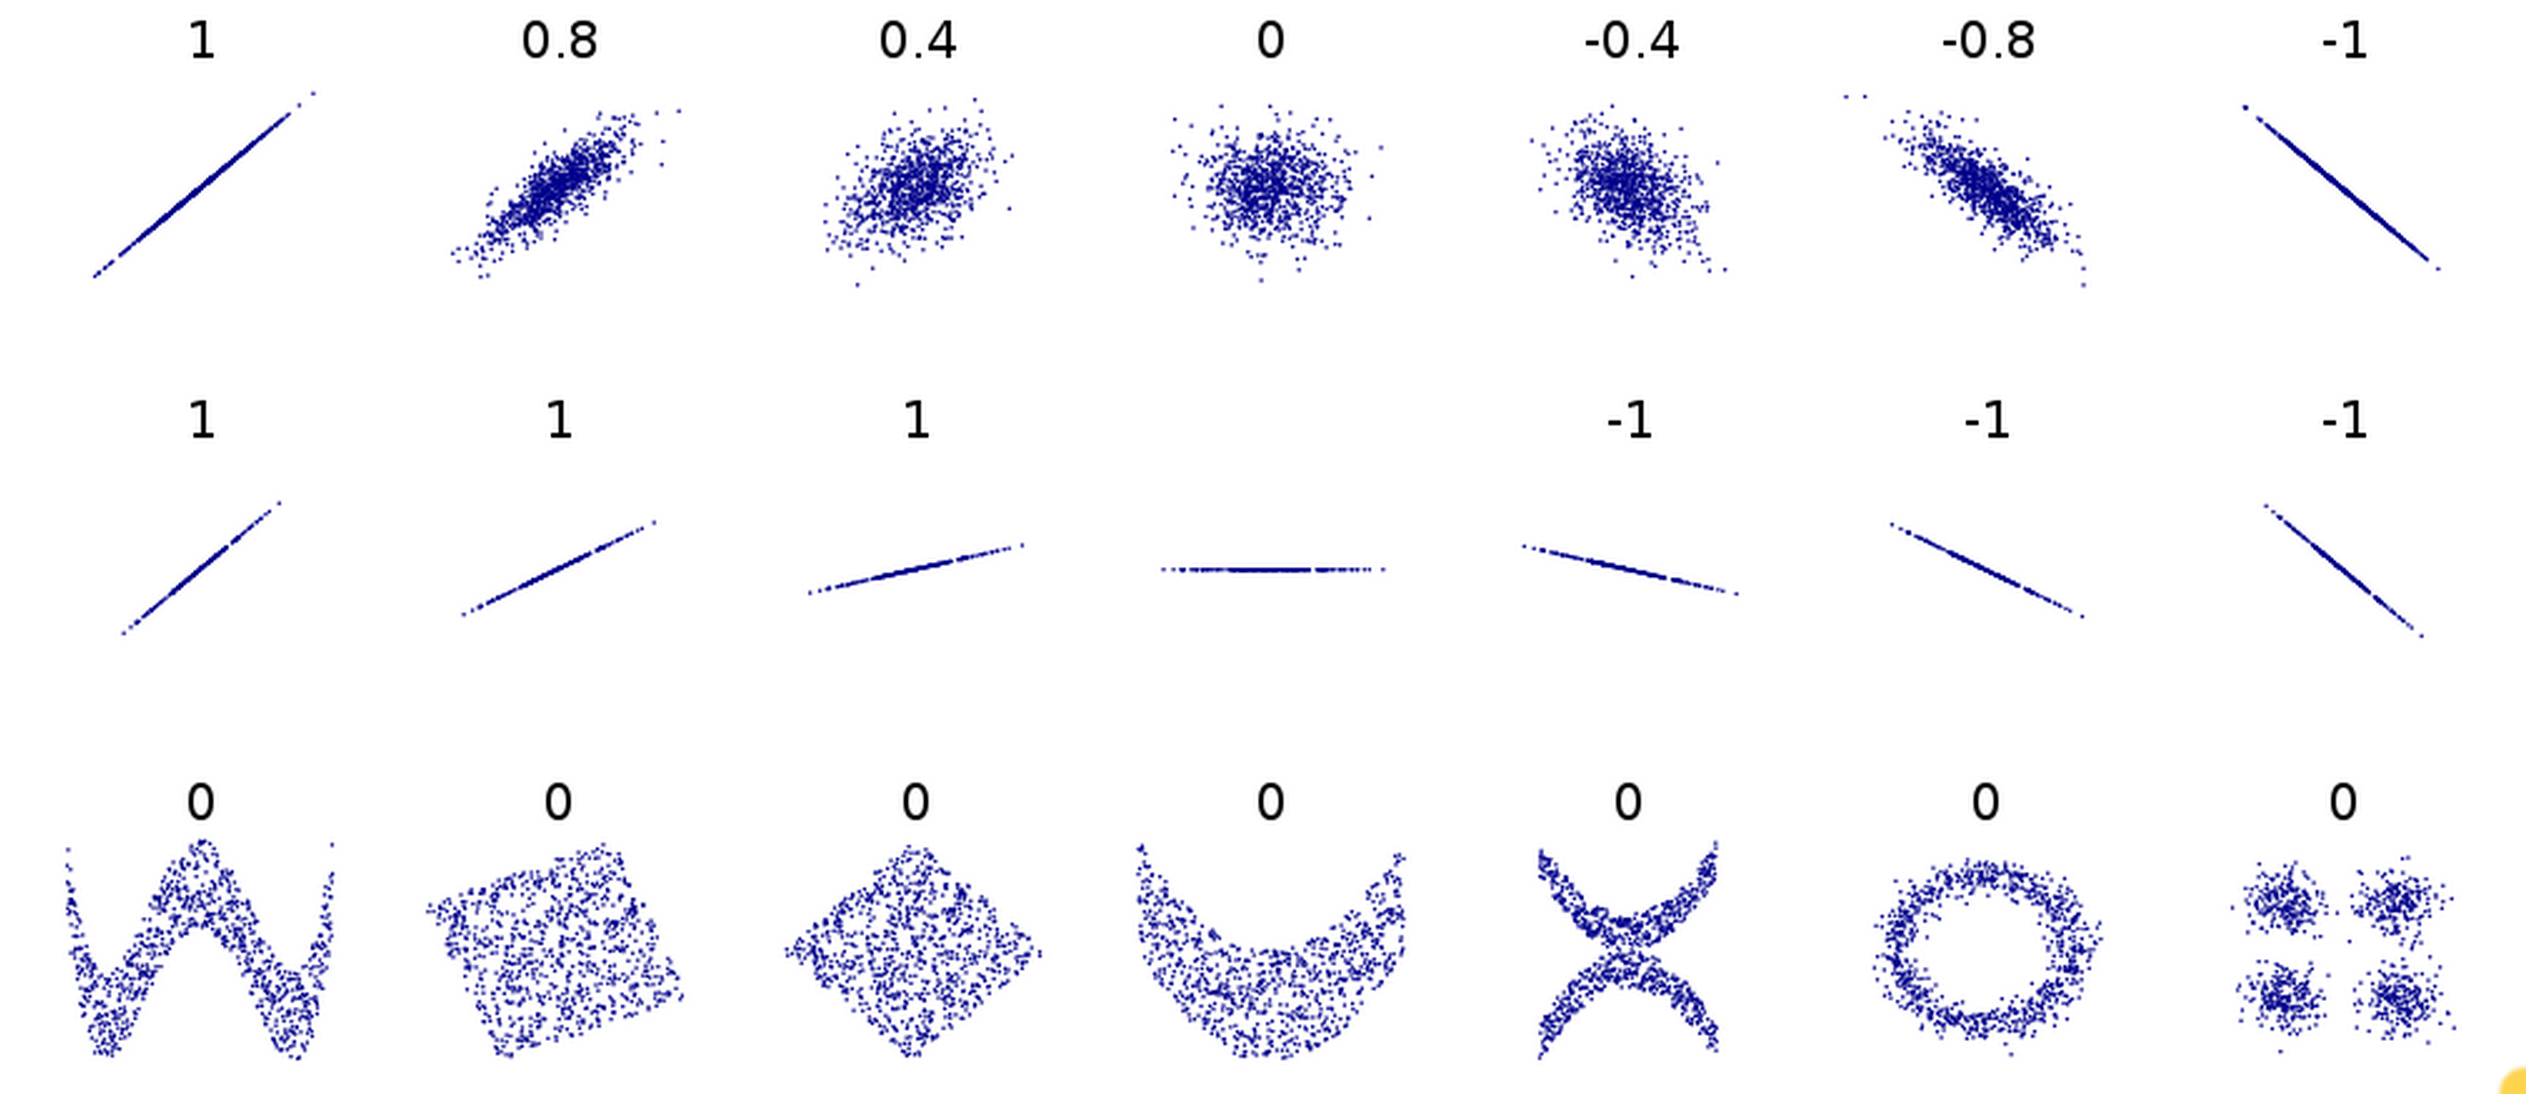
\includegraphics[width=5in]{figs/correlationCoefficients.png}
\end{center}
\caption{\label{fig:corrCoeff} Examples of joint distributions and
  their corresponding correlation coefficients. The distributions are
  represented by a sample of points drawn IID from the underlying
  distribution. The number next to each cloud of points is the value 
  of the correlation coefficients corresponding to the distribution. 
{\bf The top row} shows ellipsoidal distributions with varying levels of
correlation. {\bf The middle row} shows distributions that are concentrated
on a line of the form $X=aY$, the correlation for these distributions
is one of $-1,0,+1$ depending on the value of $a$. {\bf The bottom
  row} shows a variety of distributions where $X$ and $Y$ are
uncorrelated. These distributions demonstrate some of the many ways in
which uncorrelated random variables can be dependent.(Image taken from
WikiPedia:Correlation Coefficients)}
\end{figure}

An example of correlated random variables are the
price of fuel and the price of food. In this case there is a
direct cause and effect: fuel prices influence food prices because
manufacturing and distributing food requires large amounts of fuel. In
general, there might not be a causal relationship between two
correlated random variable. For example, consider the sentence: ``As
ice cream sales increase, the rate of drowning deaths increases
sharply. Therefore, ice cream causes drowning.''. The factual part of
the sentence is that there is a correlation between the random
variables corresponding to ``ice-cream sales'' and ``the rate of
drowning deaths''. However, the correlation does not imply
causation. The probable common cause for increases in both ice cream sales and
drowning deaths is increases in the number of people that come to the beach.  A
reminder against making this mistake is the statistical dictum
{\em ``Correlation does not imply causation''}

However, correlation {\em does} imply dependence because, as we show,
independence implies that the covariance is zero. The opposite
direction does not hold, in other words, zero covariance does not
imply that the two random variables are independent. Here is a simple
example, $X$ and $Y$ attain the values $-1,0,1$ but only the following
four combinations have non-zero probability. Specifically
\[
P(X=-1 \wedge Y=0)=
P(X=+1 \wedge Y=0)=
P(X=0 \wedge Y=-1)=
P(X=0 \wedge Y=+1)=1/4
\]
(where $\wedge$ correspond to ``and''). On the one hand, it is easy to
see that the covariance is zero, because the expected values of $X$,
$Y$ and $XY$ are all zero. On the other hand, $X$ and $Y$ are not
independent because $P(X=0 \wedge Y=0)=0$ while $P(X=0)=1/2$ and
$P(Y=0)=1/2$, and thus $P(X=0 \wedge Y=0) \neq P(X=0)P(Y=0)$

 
\chapter{Sampling, hypothesis testing, and the central limit theorem}

\section{The binomial distribution}

Let $X$ be the number of heads when a coin of bias $p$ is tossed $n$ times. 
The distribution of $X$ is so fundamental to probability and statistics that 
it merits a special name, the {\it binomial}($n,p$) distribution. Here it is,
precisely:
\begin{eqnarray*}
\Sigma     & = & \{0,1,\ldots, n\} \\
\pr(X = k) & = & {n \choose k} p^k (1-p)^{n-k}
\end{eqnarray*}
The figure below shows the binomial($100,0.6$) distribution.

\begin{center}
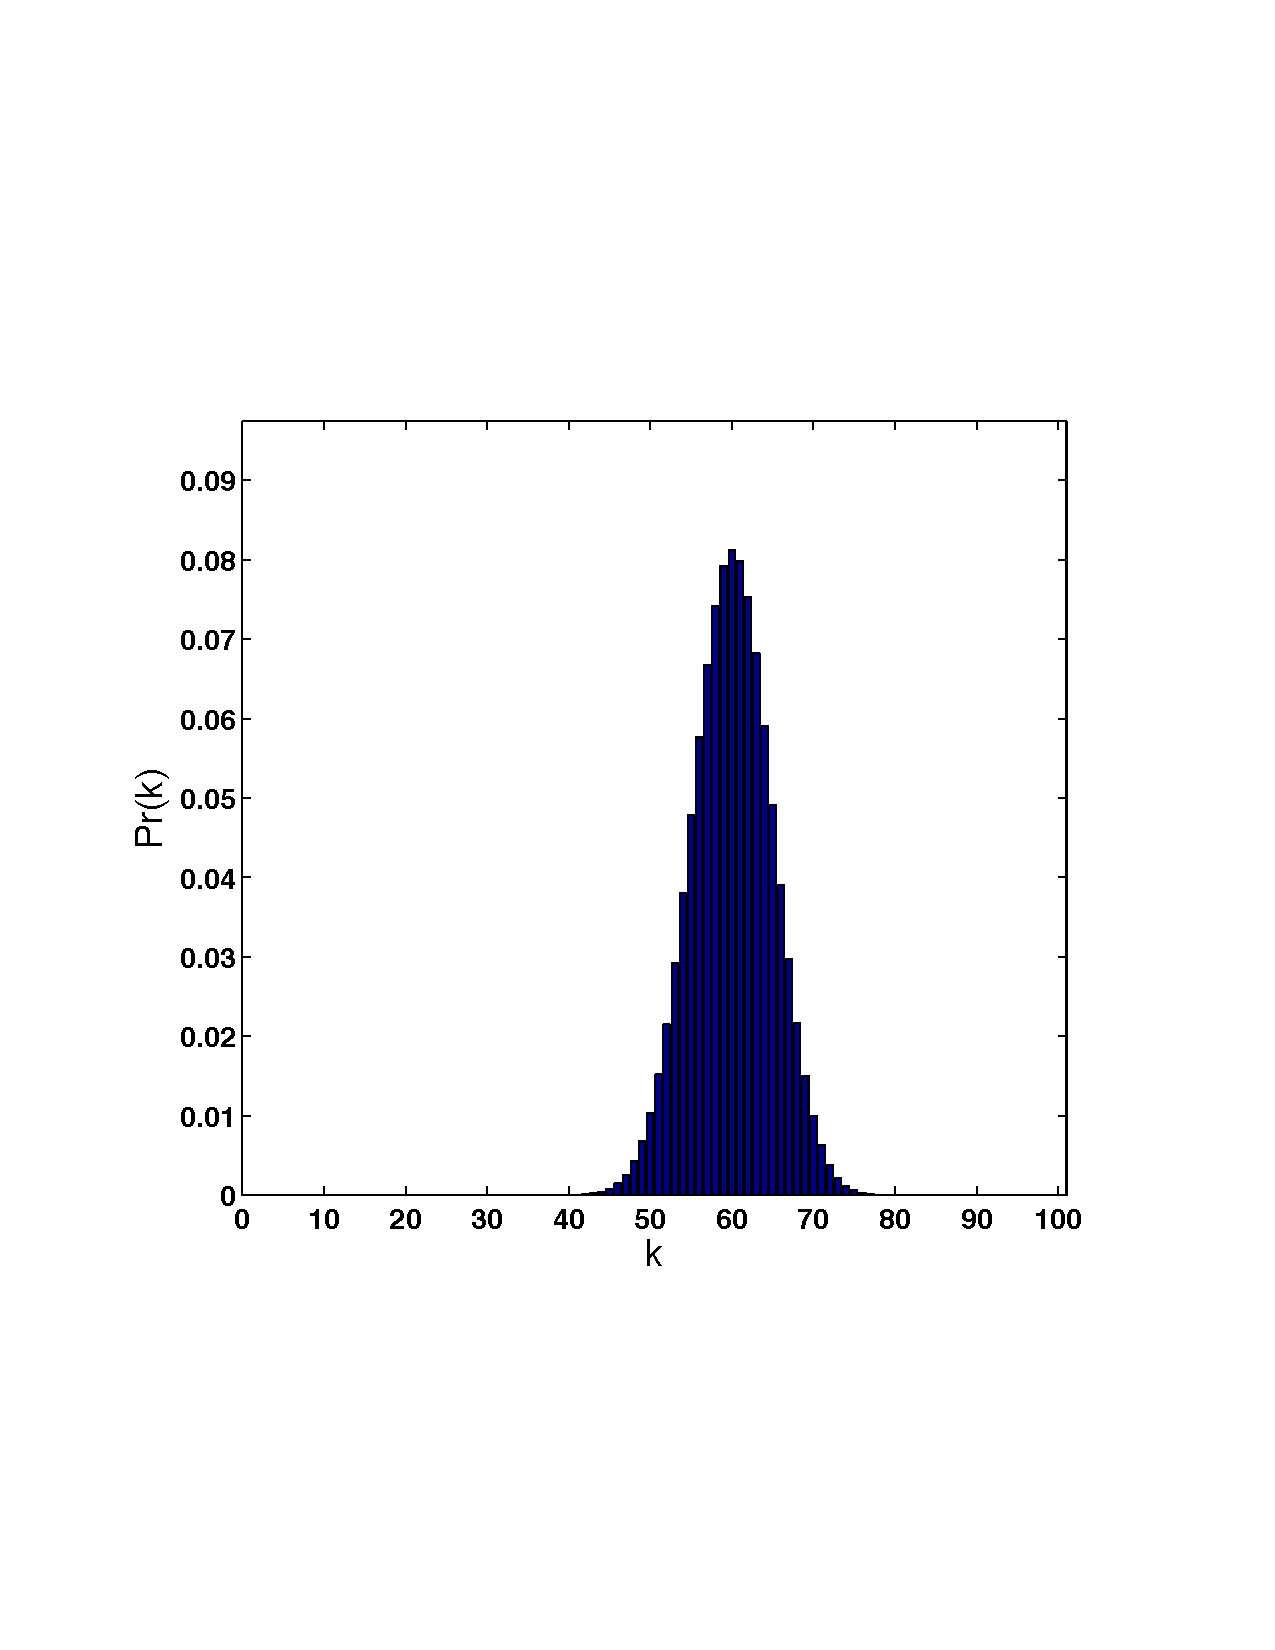
\includegraphics[width=3in]{figs/bin(100,06).pdf}
\end{center}

\noindent
The key property of this distribution is that it is tightly concentrated around
$np = 60$. This is the mean of $X$, as can be seen by writing it in the form
$X = X_1 + \cdots + X_n$, where each $X_i \sim B(p)$; in words, $X_i$ is 1 if
the $i$th coin toss comes up heads.

How spread out is the distribution? To quantify this, we need to compute the 
variance of $X$. Once again, the representation of $X$ as the sum of $X_i$'s
comes in handy, coupled with the following useful fact.
\begin{fact}
If $Z_1, \ldots, Z_n$ are independent, then 
$\var(Z_1 + \cdots + Z_n) = \var(Z_1) + \cdots + \var(Z_n)$.
\end{fact}
\noindent
Each $X_i$ has variance $p(1-p)$, so $X$ has variance $np(1-p)$ 
and thus standard deviation $\sqrt{np(1-p)}$.
\begin{fact}
If $X \sim \mbox{binomial}(n,p)$, then:
\begin{eqnarray*}
\E(X) & = & np \\
\var(X) & = & np(1-p) \\
\mbox{\rm stddev}(X) & = & \sqrt{np(1-p)}
\end{eqnarray*}
\end{fact}

There's another very useful fact about the binomial that comes up over and over again:
{\it about 95\% of the distribution lies within two standard deviations of the mean}.
That is to say,
\begin{equation}
\pr \left(np - 2 \sqrt{np(1-p)} \leq X \leq np + 2 \sqrt{np(1-p)}\right) 
\ \approx \ 0.95 . \label{eq:bin-2sigma}
\end{equation}
We'll see how this approximation arises a little later on. As an example of its use,
consider the figure shown above for binomial($100,0.6$). The standard deviation is 
$\sigma = \sqrt{100 (0.6) (0.4)} \approx 5$. And indeed almost all the 
distribution lies in the range $np \pm 2 \sigma = 60 \pm 10$.

The remarkable thing about (\ref{eq:bin-2sigma}) is that although $X$ can potentially
take on $n+1$ possible values, it effectively stays within a range of size just 
$O(\sqrt{n})$; this is miniscule compared to $n+1$ for large $n$.

\section{Hypothesis testing}

\subsection{Testing a vaccine}

Suppose there is a certain disease that cattle can contract; and that any given 
cow has a 25\% chance of contracting it within the course of a year. A new serum 
is proposed, and we want to test it to see how well it works. So we choose $n$ cows 
at random, inject them with the serum, and then keep an eye on them over the next 
year. Let's say $K$ of them remain healthy.

One possibility is that the serum has no effect whatsoever; call this hypothesis 
$H_0$. If this hypothesis is true, then the chance of infection is exactly the 
same for the cows that were injected as it is for the cow population at large, 
and thus $K \sim \mbox{binomial}(n,0.75)$.

We hope that the experiment yields a large value of $K$; this will provide evidence
against hypothesis $H_0$. But how large does $K$ need to be? It depends on how much
{\it statistical confidence} we want in our assertion that $H_0$ is false. A common
goal is a {\it 95\% confidence level}.

Suppose we have a sample of $n=100$ cows. The binomial($100,0.75$) distribution has 
mean $75$ and standard deviation $\sigma = \sqrt{100(0.25)(0.75)} \approx 4.3$. 
Using equation (\ref{eq:bin-2sigma}), we can deduce that {\it if $H_0$ were true}, 
we would expect (with 95\% confidence) a value of $K$ in the range $75 \pm 8.6$. 
If $K$ exceeds this, that is if $K > 83$, then we can reject $H_0$ with a 95\% 
confidence level.

\subsection{A blood pressure drug}

Suppose a new blood pressure drug is proposed, and to test it, a sample of
$n$ patients is selected. Their blood pressure is measured with and without
the drug.

\begin{tabular}{ccc}
Person   & B.P. with drug & B.P. without drug \\
1        & $x_1$          & $x_1'$ \\
2        & $x_2$          & $x_2'$ \\
$\vdots$ & $\vdots$       & $\vdots$ \\
$n$      & $x_n$          & $x_n'$
\end{tabular}

\noindent
The $i$th trial is called a success if $x_i < x_i'$; let $K$ be the total number
of successes. How should the evidence be evaluated?

Let $H_0$ be the hypothesis that the drug is useless. Under this hypothesis,
$K \sim \mbox{binomial}(n,0.5)$. Thus $K$ has expected value $0.5 n$ and 
standard deviation $\sqrt{n (0.5) (0.5)} = 0.5 \sqrt{n}$. As we
noted above, with 95\% confidence, we'd expect $K$ to be within two standard
deviations of its mean, that is, $K = 0.5 n \pm \sqrt{n}$.

So if $K$ exceeds $0.5n + \sqrt{n}$, we can declare that $H_0$ is invalidated
with 95\% confidence, implying that the drug is not entirely useless.

\section{Sampling}

We live in an age where the government and the mass media are continuously polling
the public. They wish to know the fraction of people who like sushi, think Obama
is doing a good job, support Tiger Woods, think God exists, feel pessimistic
about the future, smoke, think the war in Iraq is unnecessary, etc. This constant
polling affects decision-making at every level. It advises politicians on what to
say and do. It helps companies decide how to most effectively advertise their
products. It helps investors decide where to entrust their money. And so on.

In each such case, there is an unknown probability $p$ that is sought: the fraction
of people who like sushi, for instance. Determining this fraction exactly would
require asking {\it everyone}, which is prohibitively expensive. So instead a
sample of $n$ people is chosen at random, and they are each asked whether they
like sushi. Let $K$ be the number of positive responses. Then $K$ has the
binomial($n,p$) distribution, with expected value $np$ and variance $np(1-p)$.

An estimate of the fraction of sushi-lovers is $K/n$. Notice that
\begin{eqnarray*}
\E\left(\frac{K}{n}\right) & = & p \\
\var\left(\frac{K}{n} \right) & = & \frac{\var(K)}{n^2} \ \ = \ \ \frac{p(1-p)}{n} \\
\mbox{stddev}\left(\frac{K}{n}\right) & = & \sqrt{\frac{p(1-p)}{n}}
\end{eqnarray*}
A standard rule of thumb, given in equation (\ref{eq:bin-2sigma}) is that the 
estimate $K/n$ will lie within two standard deviations of its expected value 
with 95\% probability. Thus we can assert with 95\% confidence that the true 
fraction of people who like sushi is 
$$ \frac{K}{n} \pm 2 \sqrt{\frac{p(1-p)}{n}} .$$
But this doesn't make sense, since we don't know what $p$ is. A quick fix is
to notice that $p(1-p) \leq 1/4$ (the maximization can be done by calculus,
for instance), and thus a valid 95\% confidence interval is
$$ \frac{K}{n} \pm \frac{1}{\sqrt{n}} .$$
Thus a sample size of $2{,}500$ gives an estimate that is accurate to within
$1/\sqrt{n} = 0.02$ (at 95\% confidence), whereas a sample size of $10{,}000$
gives an accuracy of $0.01$.

What if we want a higher level of confidence, like 99\%, or even 99.9\%?
Equation (\ref{eq:bin-2sigma}) is no longer helpful; we need similar 
approximations for other confidence levels. It turns out that these are
easy to obtain, for any desired confidence level, using the {\it normal
approximation to the binomial distribution}.

{\bf read up to here for Wed 11/16}
\section{The normal distribution}

You are probably reading these notes in a library or cafeteria. Take a look
at the 100 or so people nearest to you. If you were to plot the heights of 
all the men, it would look kind of like this:

\begin{center}
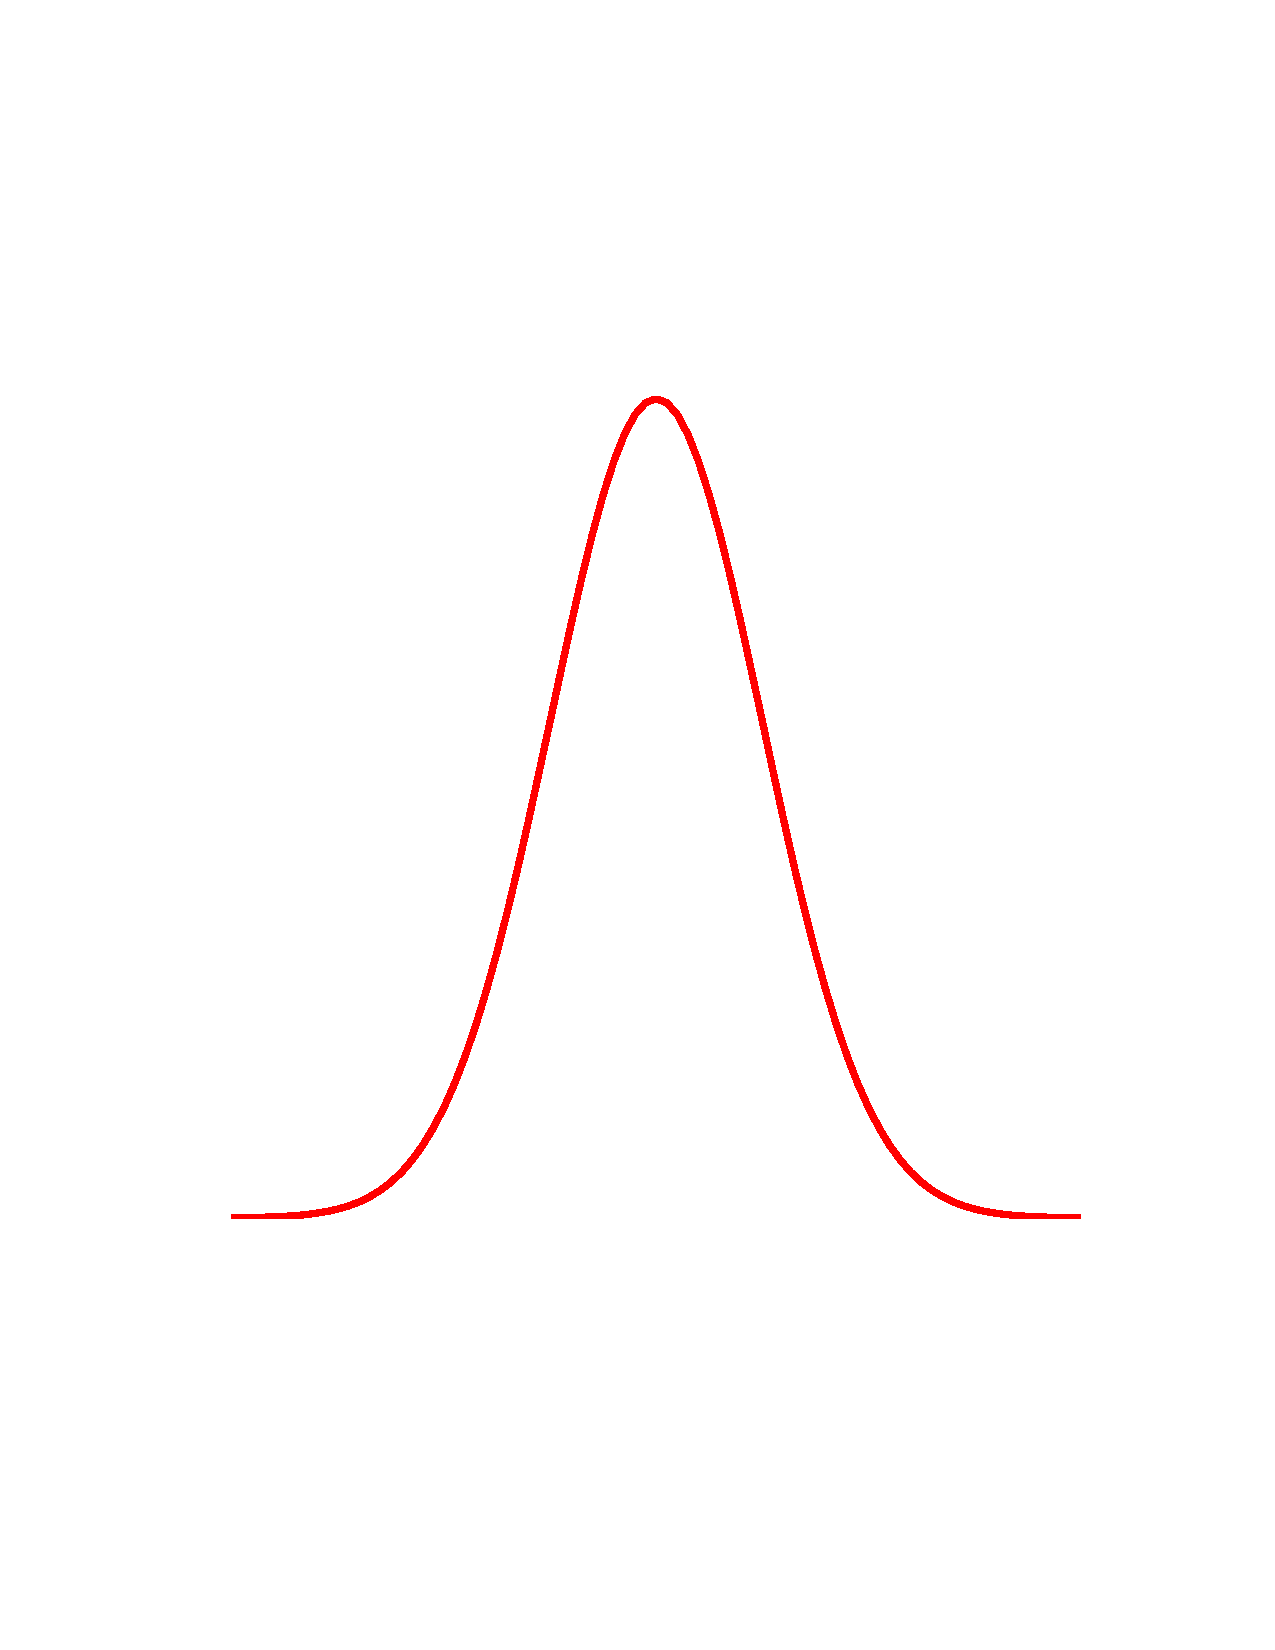
\includegraphics[width=3in,height=1.5in]{figs/bell.pdf}
\end{center}

\noindent
If you were to plot the blood pressure of all the women, it would look much 
the same. Or if you plotted the velocities of the molecules in the air, once 
again, same thing. This one distribution is everywhere. For that reason it 
is called the {\it normal} distribution.

The normal distribution with mean $\mu$ and variance $\sigma^2$ is denoted
$N(\mu, \sigma^2)$. Unlike most of the examples we've seen so far, it is
a {\it continuous} distribution, a density over the real line. The density 
at any point $x$ is
$$ \frac{1}{\sigma \sqrt{2\pi}} e^{-(x-\mu)^2/2\sigma^2} .$$
Don't worry too much about this specific functional form. Instead, let's
look at pictures of three different normal distributions.

\begin{center}
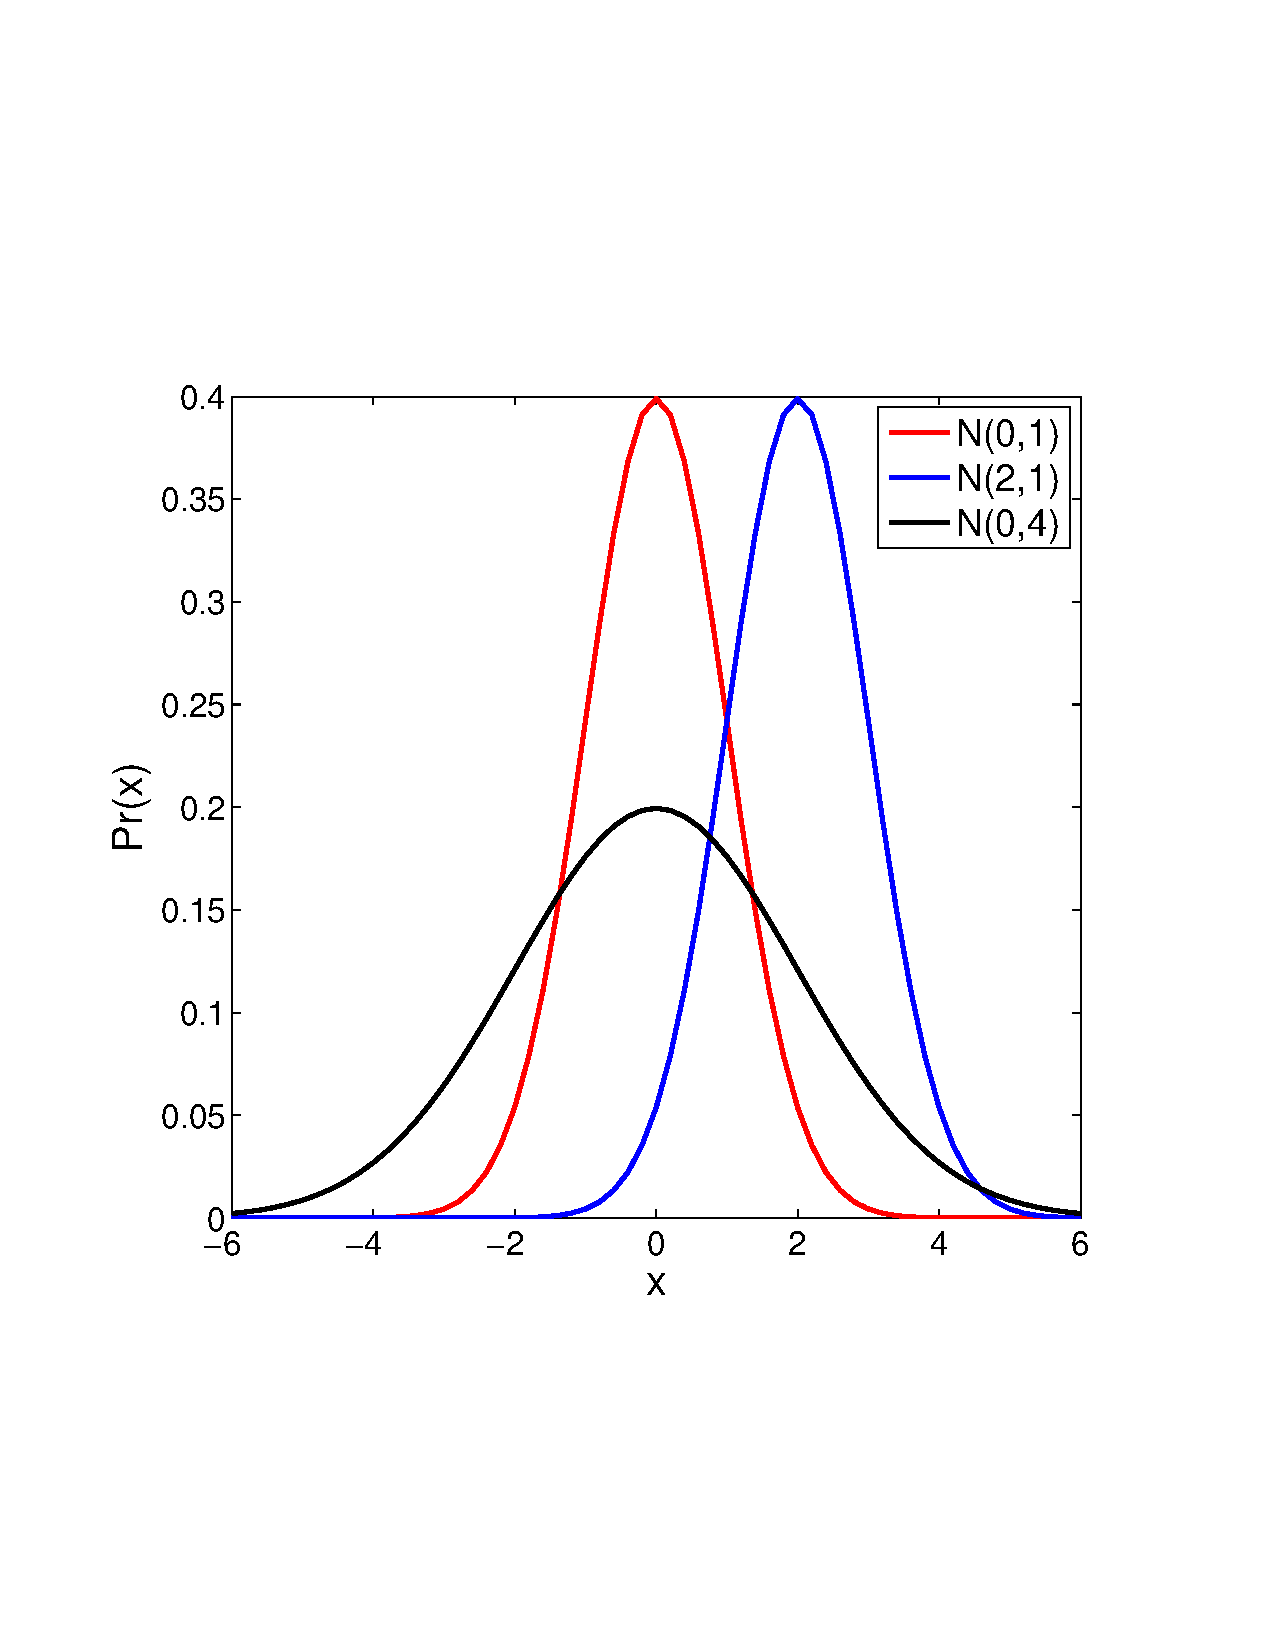
\includegraphics[width=4in,height=3in]{figs/three-norm.pdf}
\end{center}

\noindent
The red curve (or, if you're reading this in black and white, the tall curve
in the middle) is $N(0,1)$: the normal distribution with mean 0 and
variance 1. This is sometimes called the {\it standard normal}. All other
normal distributions are simply scaled and translated versions of it. For
instance, the blue curve (the one on the right) is $N(2,1)$, which is obtained
by shifting the standard normal two units to the right. The black curve (the
wide one in the middle), on the other hand, is $N(0,4)$, obtained by scaling
the standard normal by a factor of two. Here's a summary of the relationship 
between different normal distributions.
\begin{fact}
If $X \sim N(\mu, \sigma^2)$ then $aX + b \sim N(a\mu + b, a^2 \sigma^2)$.
\end{fact}

\subsection{Sums of independent random variables}

Here's an interesting fact about the normal distribution.
\begin{fact}
If $X,Y$ are independent, with $X \sim N(\mu_1, \sigma_1^2)$ and 
$Y \sim N(\mu_2, \sigma_2^2)$, then $X + Y \sim N(\mu_1+\mu_2, \sigma_1^2+ \sigma_2^2)$.
\end{fact}
In words, if a bunch of independent random variables are each normally distributed, 
and you add them up, the result still has a normal distribution.

In fact, something much more spectacular is true: even if the independent random 
variables are {\it not} normally distributed, their sum looks like a normal 
distribution! 
\begin{fact}[Central limit theorem]
Suppose $X_1, \ldots, X_n$ are independent with mean $\mu$ and variance $\sigma^2$.
Then for sufficiently large $n$, the distribution of $(X_1 + \cdots + X_n)/n$ is
approximately $N(\mu, \sigma^2/n)$. Equivalently, the distribution of 
$X_1 + \cdots + X_n$ is approximately $N(n \mu, n \sigma^2)$.
\end{fact}
This astonishing fact helps explain why the normal distribution is observed all
over the place.

\subsection{Tails of the normal}

In sampling and hypothesis testing, we ultimately end up adding independent random
variables; more on this below. Thus the result is well-approximated by the normal
distribution, and by analyzing the tails of this distribution, we can get 
intervals for any desired level of confidence.

Suppose $X \sim N(\mu,\sigma^2)$. If we want a 95\% confidence interval, we seek a 
value of $z$ for which 
$$ \pr(\mu-z \leq X \leq \mu+z) = 0.95 .$$
The answer, it turns out, is $z = 2 \sigma$. If we want a 99\% confidence interval, we
seek a value of $z$ for which
$$ \pr(\mu-z \leq X \leq \mu+z) = 0.99 .$$
In this case, $z = 3 \sigma$.

Here is a summary of some key facts about tails of the normal.
\begin{fact}
If $X \sim N(\mu, \sigma^2)$, then:
\begin{itemize}
\item With 66\% probability, $X$ lies between $\mu-\sigma$ and $\mu+\sigma$.
\item With 95\% probability, $X$ lies between $\mu-2\sigma$ and $\mu+2\sigma$.
\item With 99\% probability, $X$ lies between $\mu-3\sigma$ and $\mu+3\sigma$.
\end{itemize}
\label{fact:normal-tails}
\end{fact}

\section{Sampling revisited}

\subsection{Polls with yes/no answers}

From the population at large $n$ people are chosen at random and are asked a particular
question (``Do you approve of the corporate bailouts?''). The goal is to estimate 
the fraction $p$ of the underlying population that would answer yes. Let's say
that $K$ of the sampled people say yes; then $K \sim \mbox{binomial}(n,p)$, and
thus a reasonable estimate of $p$ is $K/n$.

To analyze the situation further, it helps to approximate the binomial by a normal
distribution. Notice that 
$$ K = X_1 + X_2 + \cdots + X_n $$
where the $X_i$ are independent $B(p)$ random variables (``did the $i$th person 
say yes?''). By the central limit theorem,
$$ \frac{K}{n} \mbox{\ is distributed like\ } N\left( p, \ \frac{p(1-p)}{n} \right) .$$
Writing $\sigma = \sqrt{\frac{p(1-p)}{n}} \leq \frac{1}{2\sqrt{n}}$, we can conclude from 
Fact~\ref{fact:normal-tails} that the estimate $K/n$ is accurate within
\begin{itemize}
\item $\frac{1}{2\sqrt{n}}$ with at least 66\% probability.
\item $\frac{1}{\sqrt{n}}$ with at least 95\% probability.
\item $\frac{3}{2\sqrt{n}}$ with at least 99\% probability.
\end{itemize}
And other confidence intervals are also easy to obtain, from standard tables of 
the normal distribution.
 
\subsection{Polls with numeric answers}

Many polls demand numeric rather than yes/no answers. How many glasses of wine do
you drink daily? What is your salary? How old are you? And so on.

Suppose, for instance, that we wish to assess the overall educational levels
(number of years of schooling) of residents of San Diego. If we were to consider 
{\it all} San Diegans of age $\geq 25$, this would be a distribution with some 
unknown mean $\mu$ and standard deviation $\sigma$. We would like to estimate 
$\mu$, the average educational level. So we randomly pick $n$ people of age 
$\geq 25$ and ask them how many years they have spent in school. Suppose their 
answers are $X_1, \ldots, X_n$.

The empirical mean (the mean of the samples) is
$$ M \ = \ \frac{X_1 + \cdots + X_n}{n} $$
and the empirical standard deviation is
$$ S \ = \ \sqrt{\frac{(X_1 - M)^2 + \cdots + (X_n - M)^2}{n}} .$$
It is reasonable to use $M$ as an estimate of $\mu$. What kind of confidence
interval can we give for it?

This is where the central limit theorem once again comes in. Since the $X_i$ are
independent, we can assert that
$$ M \mbox{\ is distributed like\ } N\left(\mu, \frac{\sigma^2}{n} \right) .$$
Thus we immediately have the following confidence intervals, from 
Fact~\ref{fact:normal-tails}.
\begin{itemize}
\item With 95\% probability, $M$ is lies between $\mu-\frac{2\sigma}{\sqrt{n}}$ and 
$\mu+\frac{2\sigma}{\sqrt{n}}$.
\item With 99\% probability, $M$ lies between $\mu-\frac{3\sigma}{\sqrt{n}}$ and 
$\mu+\frac{3\sigma}{\sqrt{n}}$.
\end{itemize}
Thus, for instance, when using $M$ to estimate $\mu$, we can be 95\% certain that 
it is accurate within $\pm \frac{2\sigma}{\sqrt{n}}$. But wait: we don't know
$\sigma$. So instead, it is customary to use the empirical standard deviation
instead, and to assert that $M$ is accurate within  $\pm \frac{2 S}{\sqrt{n}}$,
with 95\% confidence.

Returning to the schooling example, suppose we poll $n = 400$ people, and find 
that the empirical average and standard deviation are $M = 11.6$ and $S = 4.1$,
respectively. Then we can assert with 95\% confidence that the average number
of years of schooling of San Diegans is
$$ 11.6 \pm \frac{2 \times 4.1}{\sqrt{400}} \ \ = \ \ 11.6 \pm 0.41 .$$

 
\section{The Bonferroni correction}
When performing statistical test, we often want to use the same data
set to test many different alternative hypotheses. For example, when
studying high blood pressure we might want to support or refute
the following hypotheses
\begin{enumerate}
\item Blood pressure is elevated in patients with high cholesterol.
\item Blood pressure is elevated in older patients.
\item High blood pressure is caused by stress.
\item Blood pressure is elevated in patients that eat too many
  vegetables.
\item and so on.
\end{enumerate}
Suppose we run a test whose significance is $\alpha$ for each of these
hypotheses and find that one of the tests rejects the null
hypothesis. Can we say that the significance of this rejection is
$\alpha$? Clearly, as the number of tests increases, the significance
of each test decreases. How can we account for that? It is tempting to
think of passing each test as an independent event and calculate the
overall significance based on that. However, we don't know whether the
tests are independent or not. In fact, the opposite is probably true:
older patients tend to also have high cholesterol.

We therefor do the safe thing and use the union bound. Let $T_i$,
$i=1,\ldots,n$ be the event corresponding to test $i$ rejecting the
null hypothesis when the null hypothesis is in fact true. Suppose that
the $p$ value of each of the $n$ tests is at most $\alpha$,
i.e. $P(T_i) \leq \alpha$.
 
The union bound tells us that 
\[
P\left( \bigcup_{i=1}^n T_i \right) \leq \sum_{i=1}^n P(T_i) \leq n \alpha
\]

\section{Estimating the size of large populations}
Statistical techniques are useful for estimating the size of a large
population. Suppose for example that we want to count the number of
fish in a lake. How would we do that? Instead of trying to catch all
the fish, which is both impossible and damaging to the fish
population, we perform the following two phase test:
\begin{enumerate}
\item We catch fish, mark them with some non-intrusive marker, and
  release them back to the lake. Suppose we mark $m$ of them with a
  mark that sticks to the fish but does not hurt it.
\item After we marked the $m$ fish, we wait for them to mix with the
  other fish and then catch $l$ fish and count how many of these
  have been marked. We denote the number of marked fish by the random
  variable $Y$.
\end{enumerate}
The probability that each that each fish caught in the second batch is
marked is equal to the fraction of all of the fish in the lake that
are marked, which is $m/n$. This means that the random variable $Y$ is
a sum of $l$ independent binary random variables each with mean $m/n$.
Therefor the mean of $Y$ is $(lm)/n$. The standard deviation of each
of the binary variables is at most $1/2$ (which happens when
$m/n=1/2$). Thus the standard deviation of $Y$ is $\sqrt{l}/2$.
Therefor the 95\% significance interval for $(lm)/n$ is
$[Y-\sqrt{l},Y+\sqrt{l}]$.

We are interested in estimating $n$, therefor our estimate is the range.
\[
\left[\frac{lm}{Y+\sqrt{l}}, \frac{lm}{Y-\sqrt{l}} \right]
\]

Note that if the number of fish in the lake $n$ is large, so that $m/n
\approx 1/l$ then there is a good chance we will see no marked fish in
the second batch. We might need to mark more and more fish until the
chance of catching a marked fish becomes reasonably high.

          % 6 tex
\chapter{Randomized algorithms}

Randomized algorithm are algorithms that use randomization in order to
compute more efficiently. A randomized algorithm is different from a
conventional, or deterministic algorithm in that the output that
running the algorithm multiple times with the {\em same input} can
result in different traces and in different outputs. The output from a
randomized algorithm can be correct only with some non-zero
probability. The running time of the algorithm can be short only in
expectation.

Programming and debugging randomized algorithms is significantly
harder than using deterministic algorithms because errors are harder
to reproduce. It is also sometimes hard to convince management to use
an algrithm whose behaviour is unpredictable. However, the benefits of
using randomized algorithm are often substantial. In some cases, such
as Hash tables, the use of randomized algorithm is so common that it
is taken for granted.

We will present several randomized algorithm, starting with the
simplest one: finding the median.

\section{Finding percentiles}

\subsection{The mean as a summary statistic}

Suppose UCSD tracks this year's graduating class in computer science and finds out everyone's 
salary ten years down the line. What might these numbers look like? Well, if there are (say)
100 students, the spread might be roughly:
\begin{itemize}
\item A few people with zero salary (unemployed)
\item A few grad students with salary around 20K
\item A few part-timers with salary around 50K
\item A whole lot of software engineers with salaries between 100K and 200K
\end{itemize}
The {\it mean} salary would then be something like 100K, which UCSD could report with
pride in its brochure for prospective students.

Now suppose that one student managed to strike it rich and become a billionaire. 
Accordingly, take the spread of salaries above and convert one of the 200K salaries 
to 1000000K. What would be the new mean salary? Answer: at least 10 million dollars! 
(Do you see why?) If UCSD were to report this number, nobody would take it seriously,
despite its being perfectly truthful.

The problem is that the mean is extremely sensitive to {\it outliers} -- it is very 
easily thrown off by a single number that is unusually small or unusually large. In
many circumstances, therefore, the preferred summary statistic is the {\it median}, 
or 50th percentile. For the salary data, for instance, the median would remain 
unchanged (at around 100K) even if a few people were to become billionaires, or if 
a few more people were to lose their jobs.

We're also interested in other percentiles -- the 25th, 75th, and so on. How can
we compute these for a {\it very large} data set (for instance, a data set giving 
the salary of everyone in the US)?

\subsection{Selection}

Here the problem, formally.

\begin{quote}
{\sc Selection}

{\it Input:} An array $S[1\cdots n]$ of $n$ numbers; an integer $k$ between 1 and $n$

{\it Output:} The $k$th smallest number in the array.
\end{quote}
The median corresponds to $k= \lceil n/2 \rceil$, while $k=1$ retrieves the very 
smallest element. The $p$th percentile ($0 \leq p \leq 100$) can be obtained with 
$k = \lceil pn/100 \rceil$.

The most natural algorithm for this problem is:
\begin{quote}
Sort $S$ and return $S[k]$
\end{quote}
The running time here is dominated by that of sorting, which is $O(n \log n)$. This
is pretty good, but we'd like something faster since we often need to compute
percentiles of enormous data sets.

\subsection{A randomized algorithm}

Here's a randomized (and recursive) procedure for selection.

For any number $v$, imagine splitting array $S$ into three categories: 
elements smaller than $v$, those equal to $v$ (there might be duplicates), 
and those greater than $v$. Call these $S_L$, $S_v$, and $S_R$ respectively. 
For instance, if the array
$$ S :\ \ \begin{tabular}{|c|c|c|c|c|c|c|c|c|c|c|} \hline
2 & 36 & 5 & 21 & 8 & 13 & 11 & 20 & 5 & 4 & 1\\ \hline
\end{tabular}$$
is split on $v = 5$, the three subarrays generated are
$$ 
S_L :\ \  \begin{tabular}{|c|c|c|} \hline 2 & 4 & 1 \\ \hline \end{tabular} 
\hskip.4in 
S_{v} :\ \ \begin{tabular}{|c|c|} \hline 5 & 5 \\ \hline \end{tabular} 
\hskip.4in 
S_{R} :\ \ \begin{tabular}{|c|c|c|c|c|c|} \hline 36 & 21 & 8 & 13 & 11 & 20 \\ \hline
\end{tabular} 
$$
The search can instantly be narrowed down to one of these sublists. If we want, say, 
the {\it eighth}-smallest element of $S$, we know it must be the {\it third}-smallest 
element of $S_R$ since $|S_L| + |S_v| = 5$.
That is, $\mbox{\sc selection}(S, 8) = \mbox{\sc selection}(S_R,3)$.
More generally, by checking $k$ against the sizes of the subarrays, 
we can quickly determine which of them holds the desired element:
$$ 
\mbox{\sc selection}(S,k) 
\ = \ 
\left\{ \begin{array}{ll}
\mbox{\sc selection}(S_{L},k) & \mbox{if $k \leq |S_{L}|$} \\ 
v                             & \mbox{if $|S_{L}| < k \leq |S_{L}| + |S_{v}|$} \\
\mbox{\sc selection}(S_{R}, k - |S_{L}| - |S_{v}|) & \mbox{if $k > |S_{L}| + |S_{v}|$} .
\end{array} \right.
$$
The three sublists $S_{L}, S_{v}, S_{R}$ can be computed from $S$ in {\it linear} 
time, scanning left-to-right. We then recurse on the appropriate sublist. 

The effect of the split is thus to shrink the number of elements from $|S|$ to 
at most $\max\{|S_{L}|, |S_{R}|\}$. How much of an improvement is this, and 
what is the final running time?

\subsection{Running time analysis}

By how much does a single split reduce the size of the array? Well, this depends
on the choice of $v$.

\begin{enumerate}
\item {\it Worst case.} When $v$ is either the smallest or largest element in the
array, the array shrinks by just one element. If we keep getting unlucky in
this way, then
$$
\mbox{(time to process array of $n$ elements)}
\ = \ 
\mbox{(time to split)} + \mbox{(time to process array of $n-1$ elements)}.
$$
Since the time to split is linear, $O(n)$, this works out to a total running
time of $n + (n-1) + (n-2) + \cdots = O(n^2)$, which is really bad.

Fortunately, this case is unlikely to occur. The probability of consistently
picking an element $v$ which is the smallest or largest, is miniscule:
$$ \frac{2}{n} \cdot \frac{2}{n-1} \cdot \frac{2}{n-2} \cdots \frac{2}{3}
\ \approx \ 
\frac{2^n}{n!}
$$
(do you see where this expression comes from?).

\item {\it Best case.} The best possible case is that $v$ just happens to be 
the element we are looking for, that is, the $k$th smallest element in the array. 
In this case, the running time is $O(n)$, the time for a single split.

This case is also unlikely, but it is certainly a lot more likely than the worst
case. In fact, the probability of it occurring is at least $1/n$. (Why? When
might it be more than $1/n$?)

\end{enumerate}

Neither the best case nor worst case is a particularly good way to quantify the 
running time of this algorithm. A more sensible measure is the {\it expected} 
running time. Let $T(n)$ be (an upper bound on) the expected time to 
process an array of $n$ (or fewer) elements. We will now derive an expression
for it.

Call a split {\it lucky} if the resulting $S_L$ and $S_R$ both have size less 
than $3n/4$; call it {\it unlucky} otherwise. A split is lucky if $v$ lies 
somewhere between the 25th and 75th percentile of $S$, which happens with
probability exactly $1/2$.

Therefore,
\begin{eqnarray*}
T(n) 
& \leq &
\mbox{(time to split)} + \mbox{(expected time taken to process the larger of $S_L, S_R$)} \\
& \leq &
n + \pr{\mbox{(lucky split)}} \mbox{(time for array of size $\leq 3n/4$)}
 + \pr{\mbox{(unlucky split)}} \mbox{(time for array of size $n$)} \\
& \leq &
n + \frac{1}{2} T(3n/4) + \frac{1}{2} T(n)
\end{eqnarray*}
Rearranging, we get $T(n) \leq 2n + T(3n/4)$. Expanding it out, and using the formula
for the sum of a geometric series, we get
$$
T(n) 
\ \leq \ 
2n + 2 \cdot \frac{3n}{4} + 2 \cdot \frac{9n}{16} + \cdots 
\ \leq \ 
2n \left( 1 + \frac{3}{4} + \frac{9}{16} + \cdots \right) 
\ = \  
8n.
$$
Our randomized algorithm for selection has an expected {\it linear} running time!

\subsection{A randomized sorting algorithm}

There's a very popular algorithm for sorting that operates on similar principles.
It's called {\it quicksort}:
\begin{itemize}
\item Given an array $S[1\cdots n]$, pick an element $v$ from it at random.
\item Split $S$ into three pieces: 

\begin{center}
\begin{tabular}{ll}
$S_L$ & elements less than $v$ \\
$S_v$ & elements equal to $v$ \\ 
$S_R$ & elements greater than $v$
\end{tabular}
\end{center}

\item Now return $\mbox{quicksort}(S_L) \circ S_v \circ \mbox{quicksort}(S_R)$, 
where $\circ$ denotes concatenation. 
\end{itemize}

Letting $T(n)$ be the expected running time on an array of $n$ elements, we have
\begin{eqnarray*}
T(n) 
& = & \mbox{(time to split)} + \mbox{(expected time to sort $S_L$ and $S_R$)} \\
& = & n + \sum_{i=1}^n \pr(\mbox{$v$ is the $i$th smallest element in $S$}) (T(i-1) + T(n-i)) \\
& = & n + \frac{1}{n} \sum_{i=1}^n (T(i-1) + T(n-i)) .
\end{eqnarray*}
This is tricky to solve, but works out to $T(n) = O(n \log n)$.

\subsection{Two types of randomized algorithms}

Our algorithms for finding percentiles and for sorting are guaranteed to return 
the correct answer. But if you run them multiple times on the same input, their 
running times will fluctuate, even though the answer will be the same every time. 
Therefore we are interested in their {\it expected} running time. We call these 
{\it Las Vegas algorithms}.

But in the case of minimum cut we saw another type of algorithm -- called a 
{\it Monte Carlo algorithm} -- that always has the same running time on any 
given input, but is not guaranteed to return the correct answer. It merely 
guarantees that it has some probability $p > 0$ of being correct. Therefore, if 
you run it multiple times on an input, you'll get many different answers, of 
which roughly a $p$ fraction will be correct. In many cases, it is possible to
look through these answers and figure out which one(s) are right.

In a Monte Carlo algorithm, how much does the probability of success increase if you
run it multiple times, say $k$ times?
$$ \pr(\mbox{wrong every time}) \ = \ (1-p)^k \ \leq \ e^{-pk} .$$
To make this less than some $\delta$, it is enough to run the algorithm 
$(1/p) \log (1/\delta)$ times. For instance, to make the failure probability less than 
1 in a million, just run the algorithm $20/p$ times (a million is roughly $2^{20}$).

\section{Cumulative distributions and sorting in expected linear time}

\subsection{Cumulative Distribution Functions}

Our discussion so far focused on finite event spaces or event spaces
that correspond to the integers $0,1,2,\ldots$ (so-called countable
infinite sets). How do we define distributions over the real numbers?
That is an {\em uncountably} infinite set.\footnote{A set $A$ is
  uncountable if there is no one-to-one mapping from $A$ to the
  positive integers $1,2,3,4,...$. In other words, a set is
  uncountable if you cannot create a list which includes all of the
  elements in the set.}

When defining a distribution over the real it is not enough to assign
probabilities to individual points on the real line. Consider the {\em
  uniform distribution on the line segment $[0,1]$}, by which
we mean the set $\{x | 0 \leq x \leq 1\}$. We cannot assign each
point a probability larger than zero. because that would result in
$[0,1]$ an infinite probability. What we do instead is assign
probability to the line segment $0 \leq a < b \leq 1$ the probability
$b-a$. Thus for example $P([1/4,1/3])=1/3-1/4 = 1/12$.

More generally, we can define any distribution over the real line
using the {\em Cumulative Distribution Function}:
\newcommand{\CDF}{\mbox{CDF}}
\[
\CDF(a) \doteq P(x \leq a)
\]

\begin{figure}[th]
\begin{center}
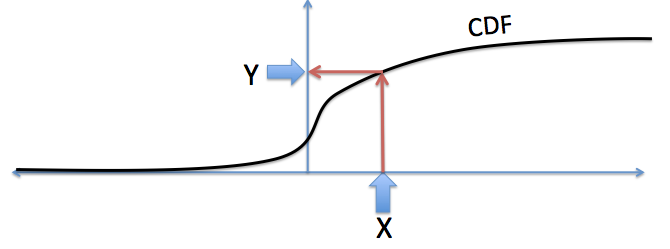
\includegraphics[width=5in]{figs/CDFmapping.png}
\end{center}
\caption{This figure depicts an example of mapping a random variable
  $X$ whose distribution is defined by a CDF (thick black curve) to
  another random variable $Y$, whose distribution is uniform in the
  interval $[0,1]$. The mapping uses the CDF as a function so that
  $Y=\CDF(X)$. \label{fig:CDFmap}}
\end{figure}

\begin{figure}[h]
\begin{center}
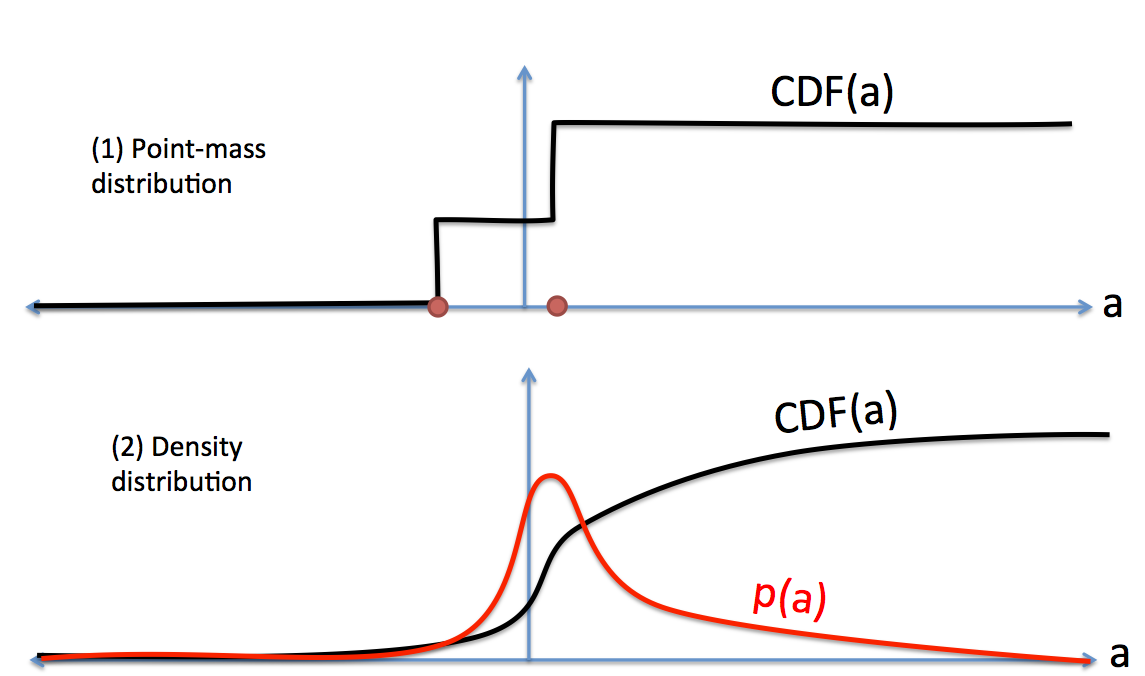
\includegraphics[width=5in]{figs/CDFs.png}
\end{center}
\caption{The CDFs for two distributions: (1) A point-mass distribution
  is a distribution that assignes non zero probabilities to two real
  values (marked by red circles) all sets that do not include at least
  one of these points have probability zero. The CDF of a point mass
  distribution is constant every where but at the point masses where
  it is discontinuous, the size of the discontinuity is the
  probability of the corresponding point. (2) A density distribution
  assigns probability zero to any single point. The CDF for such a
  distribution is a continuous increasing function that has a
  derivative. This derivative, $p(a)$ is called the {\em density function} of
  the distribution. For density distributions the CDF and the density
  function contain the same information.\label{fig:CDF}}
\end{figure}

As we see in Figure~\ref{fig:CDF} the CDF is an increasing function that
increases from zero at $-\infty$ to one at $+\infty$.

It is easy to see that $P(a<x\leq b)=\CDF(b)-\CDF(a)$.


\subsection{Examples of distributions on the real line}
If the distribution assigns a non-zero probability to some $x=a$ we
say that the distribution has a {\em point mass} at $a$. In that case
the $\CDF$ has a jump at $a$. We denote a point mass distribution
concentrated at the point $a$ by $PM(a)$. The distribution $PM(a)$
corresponds to a random variable such that $P(X=a)=1$.

\begin{figure}[t]
\begin{center}
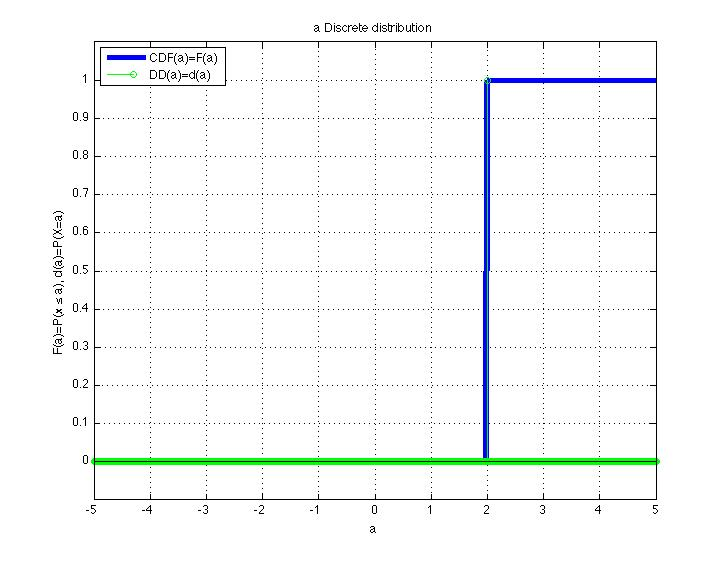
\includegraphics[width=3in]{figs/Discrete1.jpg}
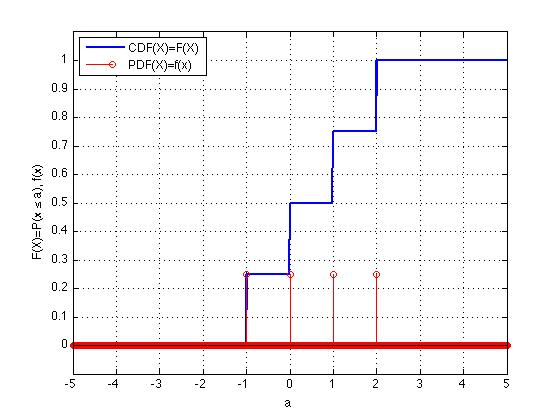
\includegraphics[width=3in]{figs/4PointMass.jpg}
\end{center}
\caption{{\bf Left:} A discrete distribution concentrated on a single
  point $P(X=2)=1$. We denote this distribution by $PM(2)$.  {\bf
    Right:} A discrete distribution distributed evenly over the four
  points $-1,0,1,2$. This distribution can be expressed as $(PM(-1)+PM(0)+PM(1)+PM(2))/4$.}
\end{figure}

\begin{figure}[b]
\begin{center}
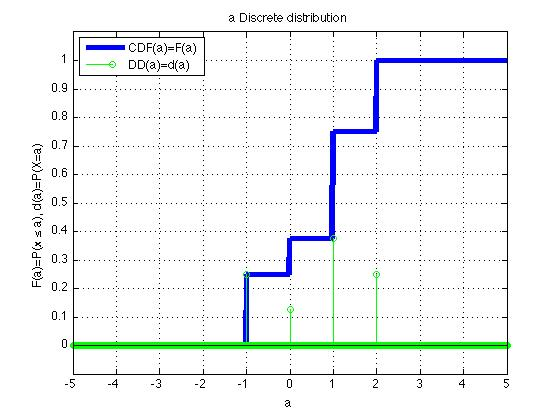
\includegraphics[width=3in]{figs/Discrete2.jpg}
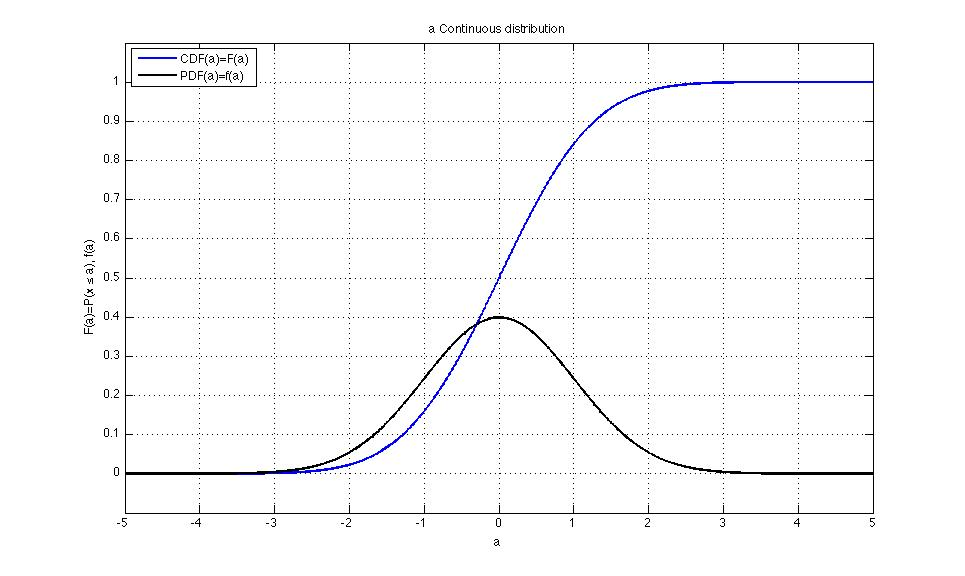
\includegraphics[width=3in]{figs/Normal.jpg}
\end{center}
\caption{{\bf Left:} A non-uniform discrete distribution. This
  distribution can be expressed as
  $(1/4)PM(-1)+(1/8)PM(0)+(5/8)PM(1)+(1/4)PM(2)$. {\bf Right:} The
  normal distribution with mean $0$ and varriance 1, denoted ${\cal
  N}(0,1)$. This is a density distribution and it's density function
is $f(x) = \frac{1}{\sqrt{2\pi}} \exp(-x^2/2)$.}
\end{figure}

\begin{figure}[t]
\begin{center}
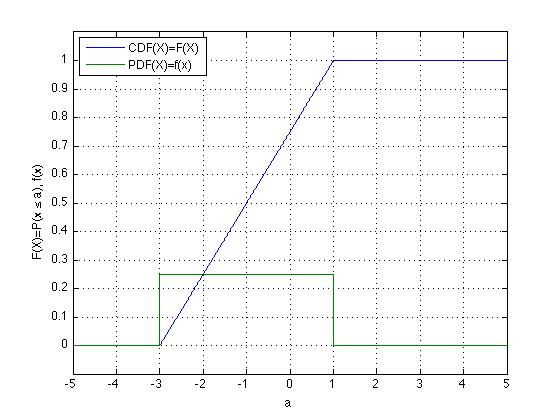
\includegraphics[width=3in]{figs/Uniform.jpg}
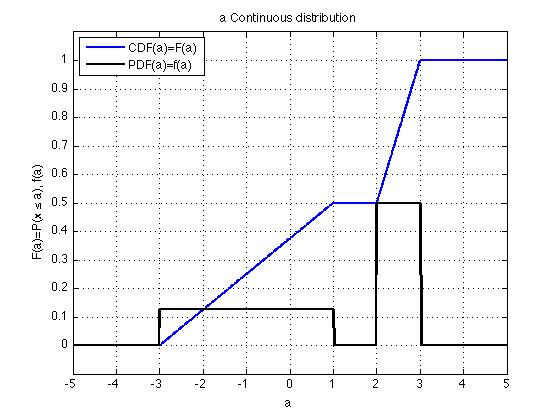
\includegraphics[width=3in]{figs/unifMixture2CDF.jpg}
\end{center}
\caption{{\bf Left:} A uniform distribution between $-3$ and $1$. We
  denote this distribution by $U(-3,1)$. {\bf Right:} A mixture of two
  uniform distributions: $(U(-3,1)+U(2,3))/2$.}
\end{figure}

\[
f(x) = \begin{cases}
0.25 & \mbox{if $ -3 \leq x \leq 1$} \\
0 & \mbox{otherwise}
\end{cases}
\]

Another important case is when the deriveative of the CDF is deifined
$p(a) = \frac{d}{dx}\left|_{x=a} \CDF(x)\right.$. The function $p(a)$
is called the {\em probability density}. Note that if $p(a)$ is
defined then, regarless of how large $p(a)$ is, $P(x=a)=0$.

When a distribution over the reals is a density distribution we can
calculate the probability of the segment $[a,b]$ using the integral:
\[
P(a < x \leq b)=\CDF(b)-\CDF(a)=\int_a^b p(x) dx
\]

\subsection{Worst-case lower bound on sorting}
You probably know of some algorithms for sorting $n$ numbers in
$O(n\log n)$ time. QuickSort and MergeSort are two such algorithms.

However, did you know that $n \log n$ is a lower bound on {\em any} sorting
algorithm? There is no sorting algorithm that can sort {\em any}
sequence of $n$ elements in time $o(n\log n)$. 

The argument is pretty simple. Let us restrict our attention to a
sequence of length $n$ that consists of the numbers $1,\ldots,n$
appearing in some order,  in other words, some permutation of the
numbers $1,\ldots,n$. As we have shown earlier in the class, there are
$n!$ such permutations.

An algorithm which sorts each of these sequences must be able to
distinguish each one of the $n!$ permutations. Suppose that the
algorithm proceeds by comparing pairs of elements in the
sequence. Each comparison has two possible outcomes. The result is a
binary tree where internal nodes correspond to comparisons and the
leaves correspond to permutations.

\begin{center}
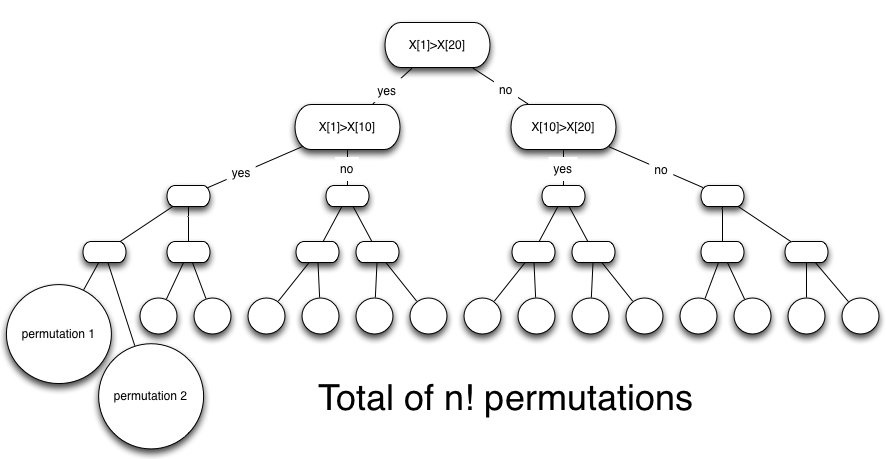
\includegraphics[width=4in]{figs/SortingLowerBound.png}
\end{center}

The depth $d$ of the tree is the worst case number of comparisons done by
the algorithm and therefor a lower bound on the worst case running
time. A basic fact about binary trees is that the number of leaves is
at most $2^d$. We there for have that $n! \leq 2^d$. Taking the
natural log of both sides and using the Strling approximation of 
$n!$ (google it!) we
find that $d \ln 2 \geq \ln n! \geq (n-1) \ln n$. We have thus found that the
worst case running time of any sorting algorithm is $\Omega(n \log n)$.

This shows that the worst case running time is $\Omega(n \log
n)$. However, as we shall see, there are sorting algorithms that,
under some statistical assumptions, take time O(n) in expectation.

\subsection{Sorting in expected linear time}

Suppose we want to sort an array of numbers $S[1\cdots n]$ that we expect to be
distributed uniformly in some range $[\min,\max]$. Here's a {\it bucket sort} approach:
\begin{itemize}
\item Divide $[\min,\max]$ into $n$ equal-sized intervals. These are the {\it buckets} 
$B_1, B_2, \ldots, B_n$.
\item Now scan array $S$ from left to right, putting each element $S[i]$ in its
appropriate bucket.
\item Return $\mbox{sort}(B_1) \circ \mbox{sort}(B_2) \circ \cdots \circ \mbox{sort}(B_n)$,
where ``sort'' is a standard sorting algorithm (say mergesort).
\end{itemize}

Notice that there is no randomization in the algorithm. However, we can talk about
the expected running time if the elements of $S$ are generated from a uniform 
distribution over $[\min,\max]$. In that case, each element is equally likely to 
fall into any of the buckets $B_i$.

Let $N_i$ be the number of array elements that fall into $B_i$. Assuming
we use a standard sorting procedure for each bucket, we get a total running time of
$$ T = N_1 \log N_1 + N_2 \log N_2 + \cdots + N_n \log N_n \ \leq \ 
N_1^2 + N_2^2 + \cdots + N_n^2 .$$

What is $\E(N_i^2)$? The easiest way to compute this is to write $N_i$ as a sum:
$$ N_i = X_1 + X_2 + \cdots + X_n$$
where $X_j$ is 1 if the array element $S[j]$ falls into bin $i$, and 0 otherwise.
Notice that $X_j^2 = X_j$, and that $X_j$ is independent of $X_{j'}$ whenever $j \neq j'$.
Therefore,
\begin{eqnarray*}
\E(X_j)  &  = & \frac{1}{n} \\
\E(X_j^2) & = & \frac{1}{n} \\
\E(X_jX_j') & = & \E(X_j) \E(X_{j'}) \ \ = \ \ \frac{1}{n^2} \mbox{\ \ \ \ if $j \neq j'$}
\end{eqnarray*}
By linearity of expectation, we then have
\begin{eqnarray*}
\E(N_i^2) 
& = & \E \left( (X_1 + \cdots + X_n)^2 \right) \\
& = & \E \left( \sum_j X_j^2 + \sum_{j \neq j'} X_j X_{j'} \right) \\
& = & \sum_j \E(X_j^2) + \sum_{j \neq j'} \E(X_j X_{j'}) \\
& = & n \cdot \frac{1}{n} + n(n-1) \frac{1}{n^2} \ \ \leq \ \ 2.
\end{eqnarray*}

So the expected running time of the sorting algorithm, once again invoking linearity, is
$$ \E(T) 
\ \leq \ \E(N_1^2) + \E(N_2^2) + \cdots + \E(N_n^2) 
\ \leq \ 2n
.$$
It is linear!

\subsection{Sorting in linear time when the distribution is known}

In the previous section we described an algorithm that can sort
elements drawn IID from the uniform distribution in expected linear
time. In this section we show how to generalize this to sorting
elements drawn IID from an arbitrary density function over the reals.

Suppose we use the CDF as a transformation, in other words, map each
$X$ to $Y=\CDF(X)$. $Y$ is a new random variable, see
figure~\ref{fig:CDFmap}. What is the distribution of the random
variable $Y$? First, it is clear that $0 \leq Y \leq 1$ because that
is the range of cumulative distribution function. We need to also
assume that the CDF is a {\em reversible} function. I.e. for any real
in the range: $0<c<1$ there exists an inverse $b=\CDF^{-1}(c)$ such
that $\CDF(b)=c$. A sufficient condition for this to hold is that the
distribution over $R$ is defined by a density function.

To understand the distribution of $Y$, let us calculate the
probability that $Y$ is in some range $c<Y<d$, where $0<c<d<1$.
Using the definition of $\CDF^{-1}$ we get
\begin{equation} \label{eqn:CDF}
P(c \leq Y \leq d) = P(\CDF^{-1}(c) \leq X \leq \CDF^{-1}(d)) =
\CDF(\CDF^{-1}(d))-\CDF(\CDF^{-1}(c)) = d-c
\end{equation}
Where the first equality is justified by the definition of
$\CDF^{-1}$, the second by the formula for calculating the probability
of a segment using the CDF, and the fourth by the cancellation :
$\CDF^{-1}(\CDF(X))=X$.  We find that the distribution of $Y$ is
uniform between 0 and 1, under the condition that the CDF is invertible.

It might help to consider a particular CDF as an example. Suppose the
CDF of $X$ is $\CDF(x) = \frac{1}{1+e^{-x}}$, this function is
invertible and it's inverse is
$\CDF^{-1}(y)=\ln\left(\frac{1}{y}-1\right)$. Apply the steps of
Equation~(\ref{eqn:CDF}) to convince yourself the it works.

Recall that we have an efficient algorithm for sorting numbers that
are distributed uniformly in some segment $[\min,\max]$.
If we know the CDF of the distribution that is generating the
numbers we wish to sort, we can map these numbers to the rannge
$[0,1]$ and then use the method suggested in the first section to sort
them in $O(N)$ time.

\section{Karger's minimum cut algorithm}

\subsection{Clustering via graph cuts}

Suppose a mail order company has the resources to prepare two different versions of 
its catalog, and it wishes to target each version towards a particular sector of its 
customer base. The data it has is a list of its regular customers, along with their 
purchase histories. How should this set of customers be partitioned into two coherent 
groups?

One way to do this is to create a graph with a node for each of the regular customers,
and an edge between any two customers whose purchase patterns are similar. The goal is
then to divide the nodes into two pieces which have very few edges between them.

More formally, the {\it minimum cut} of an undirected graph $G = (V,E)$ is a partition
of the nodes into two groups $V_1$ and $V_2$ (that is, $V = V_1 \cup V_2$ and, 
$V_1 \cap V_2 = \emptyset$), so that the number of edges between $V_1$ and $V_2$ is
minimized. In the graph below, for instance, the minimum cut has size two and partitions
the nodes into $V_1 = \{a,b,e,f\}$ and $V_2 = \{c,d,g,h\}$.

\begin{center}

\includegraphics[width=1.5in]{figs/mincut}
\end{center}

\subsection{Karger's algorithm}

Here's a randomized algorithm for finding the minimum cut:

\begin{itemize}
\item Repeat until just two nodes remain:
\begin{itemize}
\item Pick an edge of $G$ at random and collapse its two endpoints into a single node
\end{itemize}
\item For the two remaining nodes $u_1$ and $u_2$, set 
$V_1 = \{\mbox{nodes that went into $u_1$}\}$ and 
$V_2 = \{\mbox{nodes in $u_2$}\}$
\end{itemize}
An example is shown in Figure~\ref{fig:karger}. Notice
how some nodes end up having multiple edges between them.

\begin{figure}
\begin{center}
\begin{tabular}{cp{.25in}p{2.5in}} \\ \hline


\includegraphics[width=1.5in]{figs/mincut.pdf}
&
&
\raisebox{.4in}
{\begin{minipage}[c]{2.5in}
14 edges to choose from \\
Pick $b-f$ (probability $1/14$)
\end{minipage}}
\\ \hline

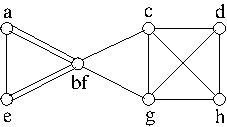
\includegraphics[width=1.5in]{figs/cut1.pdf}
&
&
\raisebox{.4in}
{\begin{minipage}[c]{2.5in}
13 edges to choose from \\
Pick $g-h$ (probability $1/13$)
\end{minipage}}
\\ \hline

\includegraphics[width=1.5in]{figs/cut2.pdf}
&
&
\raisebox{.4in}
{\begin{minipage}[c]{2.5in}
12 edges to choose from \\
Pick $d-gh$ (probability $1/6$)
\end{minipage}}
\\ \hline

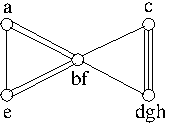
\includegraphics[width=1.25in]{figs/cut3.pdf}
&
&
\raisebox{.4in}
{\begin{minipage}[c]{2.5in}
10 edges to choose from \\
Pick $a-e$ (probability $1/10$)
\end{minipage}}
\\ \hline

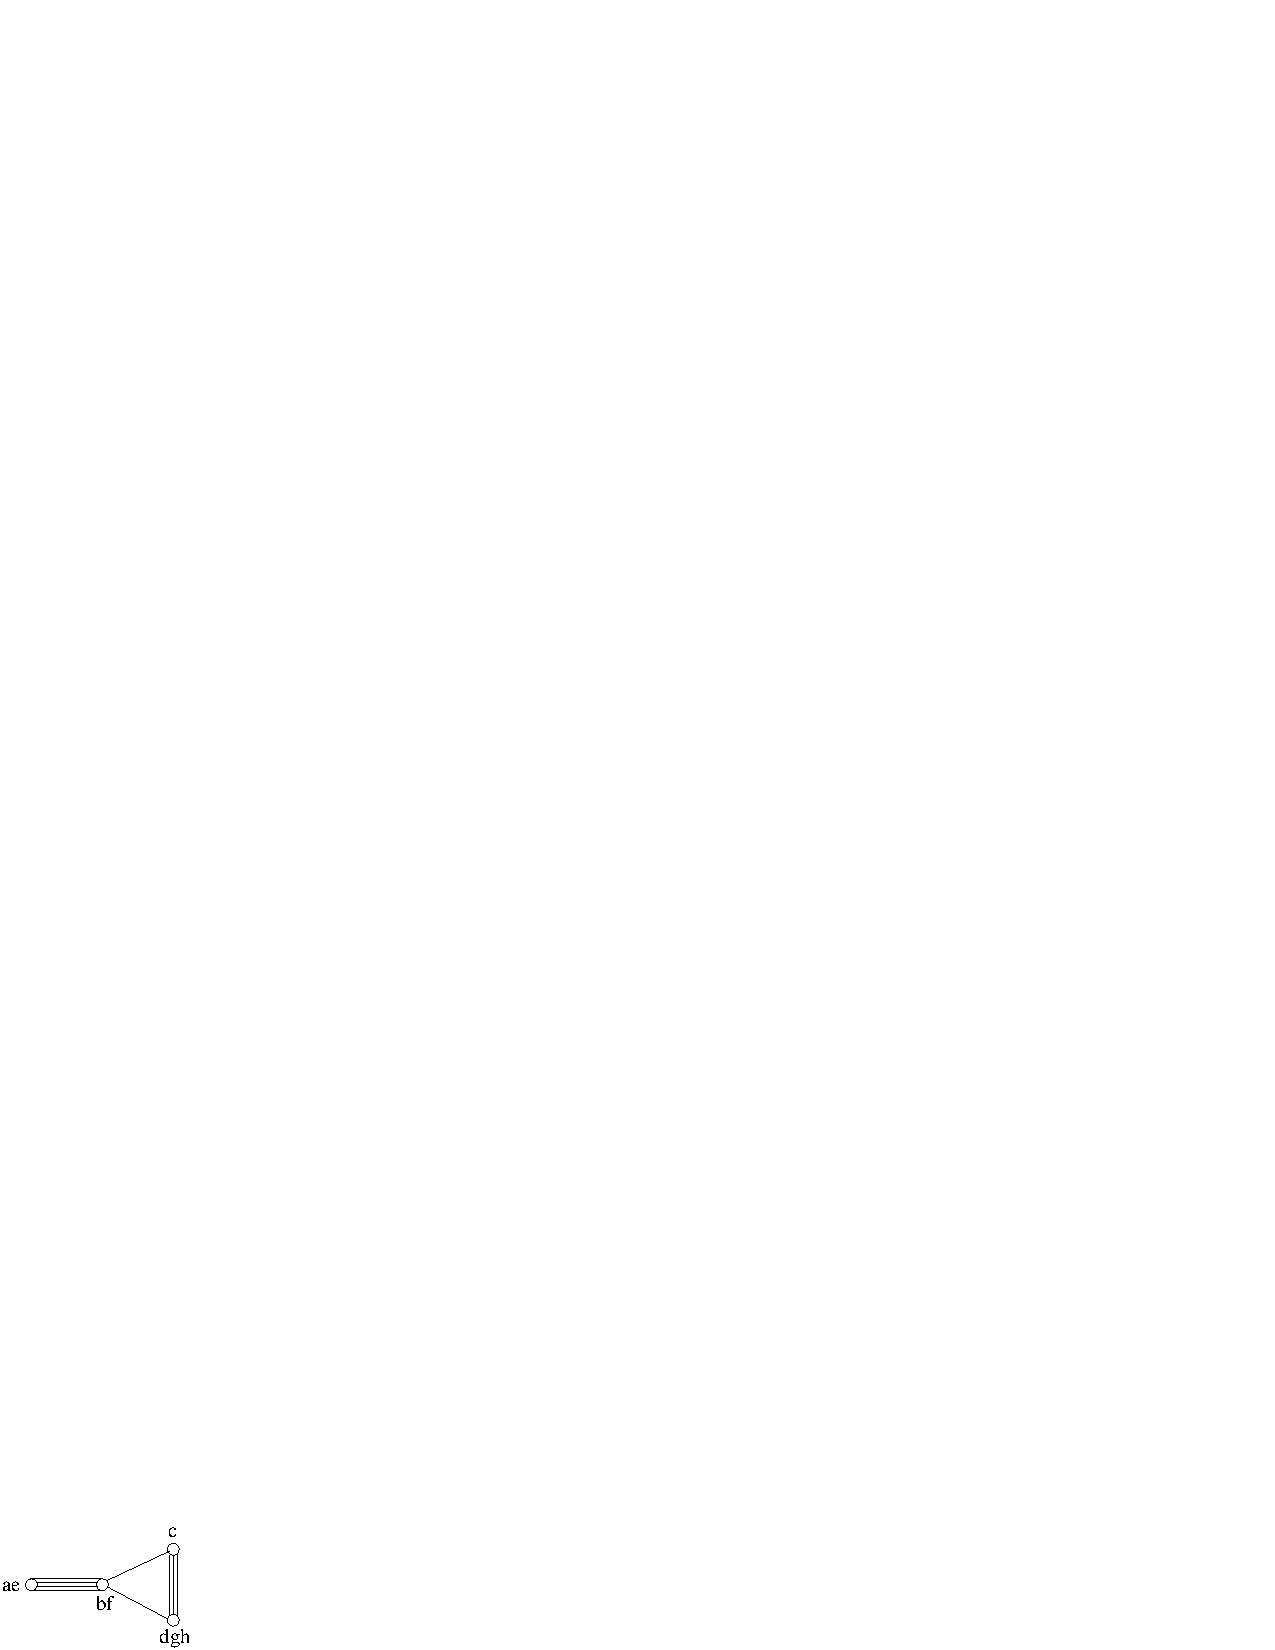
\includegraphics[width=1.35in]{figs/cut4.pdf}
&
&
\raisebox{.4in}
{\begin{minipage}[c]{2.5in}
9 edges to choose from \\
Pick $ab-ef$ (probability $4/9$)
\end{minipage}}
\\ \hline

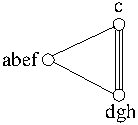
\includegraphics[width=1in]{figs/cut5.pdf}
&
&
\raisebox{.4in}
{\begin{minipage}[c]{2.5in}
5 edges to choose from \\
Pick $c-dgh$ (probability $3/5$)
\end{minipage}}
\\ \hline


\includegraphics[width=1.25in]{figs/cut6.pdf}
&
&
\raisebox{.05in}
{\begin{minipage}[c]{2.5in}
Done: just two nodes remain
\end{minipage}}
\\ \hline
\end{tabular}
\end{center}
\caption{Karger's algorithm at work.}
\label{fig:karger}
\end{figure}



\subsection{Analysis}

Karger's algorithm returns the minimum cut with a certain probability. To analyze it,
let's go through a succession of key facts.

\begin{fact}
If $\mbox{degree}(u)$ denotes the number of edges touching node $u$, then
$$ \sum_{u \in V} \mbox{degree}(u) = 2|E|.$$
\end{fact}
To see this, imagine the following experiment: for each node, list all the edges touching 
it. The number of edges in this list is exactly the left-hand sum. But each edge appears 
exactly twice in it, once for each endpoint.

\begin{fact}
If there are $n$ nodes, then the average degree of a node is $2|E|/n$.
\end{fact}
This is a straightforward calculation: when you pick a node $X$ at random,
$$ 
\E[\mbox{degree}(X)] 
\ = \ 
\sum_{u \in V} \pr(X = u) \mbox{degree}(u) 
\ = \ 
\frac{1}{n} \sum_u \mbox{degree}(u) 
\ = \ 
\frac{2|E|}{n}
$$
where the last step uses the first Fact.

\begin{fact}
The size of the minimum cut is at most $2|E|/n$.
\end{fact}
Consider the partition of $V$ into two pieces, one containing a single node $u$, and the 
other containing the remaining $n-1$ nodes. The size of this cut is $\mbox{degree}(u)$.
Since this is a valid cut, the minimum cut cannot be bigger than this. In other words,
for all nodes $u$,
$$ \mbox{(size of minimum cut)} \leq \mbox{degree}(u) .$$
This means that the size of the minimum cut is also $\leq$ the average degree, which 
we've seen is $2|E|/n$.

\begin{fact}
If an edge is picked at random, the probability that it lies across the minimum cut is 
at most $2/n$.
\end{fact}
This is because there are $|E|$ edges to choose from, and at most $2|E|/n$ of them are
in the minimum cut.
\\

Now we have all the information we need to analyze Karger's algorithm. It returns the
right answer {\it as long as it never picks an edge across the minimum cut}. If it always 
picks a non-cut edge, then this edge will connect two nodes on the same side of the cut,
and so it is okay to collapse them together.

Each time an edge is collapsed, the number of nodes decreases by 1. Therefore,
\begin{eqnarray*}
\pr(\mbox{final cut is the minimum cut})
& = &
\pr(\mbox{first selected edge is not in mincut}) \times \\
& & \pr(\mbox{second selected edge is not in mincut}) \times \cdots \\
& \geq & 
\left( 1 - \frac{2}{n} \right) \left( 1 - \frac{2}{n-1} \right) 
\left( 1 - \frac{2}{n-2} \right) \cdots \left( 1 - \frac{2}{4} \right) 
\left( 1 - \frac{2}{3} \right) \\
& = & 
\frac{n-2}{n} \cdot \frac{n-3}{n-1} \cdot \frac{n-4}{n-2} \cdots \frac{2}{4} \cdot 
\frac{1}{3} \\
& = & 
\frac{2}{n(n-1)} .
\end{eqnarray*}
The last equation comes from noticing that almost every numerator cancels with the 
denominator two fractions down the line.

Karger's algorithm succeeds with probabililty $p \geq 2/n^2$. Therefore,
it should be run $\Omega(n^2)$ times, after which the smallest cut found should
be chosen.

Those who are familiar with minimum spanning tree algorithms might be curious to
hear that another way to implement Karger's algorithm is the following:
\begin{itemize}
\item Assign each edge a random weight
\item Run Kruskal's algorithm to get the minimum spanning tree
\item Break the largest edge in the tree to get the two clusters
\end{itemize}
(Do you see why?) Over the decades, the running time of Kruskal's algorithm has 
been thoroughly optimized via special data structures. Now this same technology 
can be put to work for cuts!

\section{Hashing}

In many situations, such as a dictionary application, we need to store a vast 
collection of items in such a way that we can look up any item instantaneously. 
The way to do this is by {\it hashing}.

\subsection{The hashing framework}

Suppose you have a large collection of items $x_1, \ldots, x_n$ that you want 
to store (for instance, all English words), where these items are 
drawn from some set $\U$ (for instance, the set of all conceivable words). 
The requirements are:
\begin{enumerate}
\item The total storage space used should be $O(n)$.
\item Given a query $q \in \U$, it should be possible to {\it very rapidly}
determine whether $q$ is one of the stored items $x_i$.
\end{enumerate}

\subsection{A simple solution using randomization}

\begin{enumerate}
\item Pick a completely random function $h: \U \rightarrow \{1,2,\ldots, n\}$. 

This is the {\it hash function}. 

\item Create a table $T$ of size $n$, each of whose entries is a pointer to a 
linked list, initialized to null. 

\item Store each $x_i$ in the linked list at $T[h(x_i)]$.

We say $x_i$ {\it hashes to} location $h(x_i)$.

\item Given a query $q$, look through the linked list at $T[h(q)]$ to see if
it's there.
\end{enumerate}

Here's a picture of the data structure.

\begin{center}
%%\resizebox{2.25in}{!}{\input{figs/table.pstex_t}}
\end{center}

The storage used is $O(n)$. What about the query time?

\subsection{Average query time}

Suppose query $q$ is picked at random, so that it is equally likely to hash to
any of the locations $1,2,\ldots, n$. What is the expected query time?
\begin{eqnarray*}
\mbox{Expected query time}
& =& 
\sum_{i=1}^n \pr(\mbox{$q$ hashes to location $i$}) \cdot \mbox{(length of list at $T[i]$)} \\
& =&
\frac{1}{n} \sum_i  \mbox{(length of list at $T[i]$)} \\ 
& = & 
\frac{1}{n} \cdot n \ = \ 1
\end{eqnarray*}
So the average query time is constant!

\subsection{Worst case query time, and a balls-in-bins problem}

What is the worst case query time; that is, what is the length of the
longest linked list in $T$? Equivalently, when you throw $n$ balls in
$n$ bins, what is the size of the largest bin? We'll see that with
very high probability, no bin gets $\geq \log n$ balls.

For any bin $i$, let $E_i$ be the event that it gets $\geq \log n$ balls.
$$ \pr(E_i) \  \leq \ {n \choose \log n} \left( \frac{1}{n} \right)^{\log n} .$$
(Do you see why?) 

To upper bound this probability we use the inequality (see cheat sheet) that
\[
{n \choose k} \leq \left( \frac{ne}{k} \right)^k
\]
Applying this inequality we get:
\[
{n \choose \log n} \left( \frac{1}{n} \right)^{\log n} \leq 
\left( \frac{ne}{n \log n}  \right)^{\log n} =
\left( \frac{e}{\log n}  \right)^{\log n} =
\frac{n^{\log e}}{(\log n)^{\log n}} \leq \frac{1}{n^2}
\]
Where the last inequality can be shown by moving the $n$ from the left
to the right and taking $1/x$ and then log of both sides:
\[
(\log n)(\log \log n) \geq (2+\log e) \log n
\]
Which holds when $n>2000$

Having shown that $\pr(E_i) \leq 1/n^2$, it follows that
$$ \pr(\mbox{some bin gets $\geq \log n$ balls})
\ = \ 
\pr(E_1 \cup E_2 \cup \cdots \cup E_n)
\ \leq \ 
\pr(E_1) + \cdots + \pr(E_n) 
\ \leq \ 
\frac{1}{n}.
$$
For instance, if you throw a million balls into a million bins, then the chance that
there is a bin with $\geq 20$ balls is at most 1 in a million.

Getting back to hashing, this means that the worst case query time is (with high
probability) $O(\mbox{log} n)$.

\subsection{The power of two choices}

Here's a variant on the balls and bins setup. As usual, you have before you a 
row of $n$ bins, along with a collection of $n$ identical balls. But now, 
when throwing each ball, {\it you pick two bins at random and you put the
ball in whichever of them is less full}.

It turns out, using an analysis that is too complicated to get into here, that
under this small change, the maximum bin size will be just $O(\log \log n)$ 
instead of $O(\log n)$.

This inspires an alternative hashing scheme:

\begin{enumerate}
\item Pick {\it two} completely random functions $h_1, h_2: \U \rightarrow \{1,2,\ldots, n\}$. 

\item Create a table $T$ of size $n$, each of whose entries is a pointer to a 
linked list, initialized to null. 

\item For each $x_i$, store it in either the linked list at $T[h_1(x_i)]$ or $T[h_2(x_i)]$,
whichever is shorter.

\item Given a query $q$, look through {\it both} the linked list at $T[h_1(q)]$ and
at $T[h_2(q)]$ to see if it's there.
\end{enumerate}

The storage requirement is still $O(n)$, the average query time is still $O(1)$, but now
the worst case query time drops to $O(\log \log n)$.

\section{Information retrieval}

When you go to Google and enter a query, like
\begin{quote}
{\tt what are treatment options for pneumonia}
\end{quote}
or
\begin{quote}
{\tt new song by radiohead}
\end{quote}
you immediately get back a list of highly suitable pages. It's as if the search engine
were instantaneously able to look through the tens of billions of pages on the web and
find the relevant ones. How does it pull this off? The answer is, by a combination of
clever preprocessing, statistics, hashing, and clustering.

In fact, these basic techniques apply not just to web search but to any system for
{\it information retrieval}: answering unstructured queries about a large collection
of documents.

\subsection{Preprocessing}

There are at five crucial preprocessing steps for a search engine.
\begin{enumerate}
\item Give each webpage a {\it reliability score}.

Most of the ``information'' on the web is grossly unreliable: spam, ignorant ravings, unfounded conjectures, and idle gossip. But we'll see (a bit later in the course) that it is possible to assess the reliability or authoritativeness of individual webpages --- by analyzing the statistics of linkage patterns.

\item Ignore {\it near-duplicates} of webpages.

More on this very shortly.

\item Discover the set of {\it terms}.

A {\it term} is an individual word, or a sequence of words that should be considered together, such as {\tt Katy Perry} or {\tt Rage Against the Machine}. Terms can be discovered by analyzing co-occurrence patterns. If a sequence of $k$ words keeps occurring together, they should be designated a term.

\item Create the {\it postings list}.

This is a hash table in which each term is associated with a linked list of the pages containing it.

\begin{center}
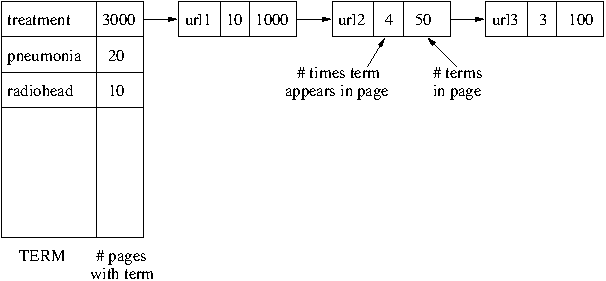
\includegraphics[width=5in]{figs/postings.pdf}
\end{center}

Each linked list is arranged in decreasing order of ``priority'' (some notion that takes into account reliability scores), and is usually truncated at a certain point.

\item Compute {\it term frequencies}.

How common is each term?

\end{enumerate}

\subsection{Answering a query}

The first step in answering a query is to order query terms by importance. The important terms are those that are uncommon. For instance, in
\begin{quote}
{\tt what are treatment options for pneumonia}
\end{quote}
the most important term is {\tt pneumonia}, since this is the least common. Next comes {\tt treatment}, and then {\tt options}. The remaining words are so common that they can be ignored.

The next step is to look at the postings list, and get all pages containing the important query term(s). Then, assign each a score based on:
\begin{itemize}
\item the reliability of that page
\item which of the important query terms it contains
\item the number of times each query term appears on that page, divided by the length of the page
\end{itemize}

This yields an ordered list of webpages, starting with the ``most relevant''. But the list will typically contain way too many pages. So they need to be clustered, and the user can then be presented with one representative page from each cluster, with the option to select ``more like this''.

For instance, pages about {\tt Rome} might be clustered into categories based on whether they refer to:
\begin{itemize}
\item Ancient Rome
\item Modern Rome
\item The TV series ``Rome''
\item and so on.
\end{itemize}

\section{Detecting near-duplicates}

Near-duplication is pervasive in the web: there are large numbers of distinct URLs which have exactly
the same content but differ only in unimportant details like headers and footers. The user of a search
engine would not be pleased if the answer to his query was a set of 10 near-identical pages! In order
to remove this redundancy, we need to define a notion of {\it similarity} between documents.

\subsection{The similarity between two documents}

For any document---call it $d$---let the set of all words in $d$ be denoted $C(d)$. For two documents 
$d$ and $d'$, we will measure their similarity by the function
$$ S(d,d') \ = \ \frac{|C(d) \cap C(d')|}{|C(d) \cup C(d')|} .$$
If the two documents are truly identical, $S(d,d') = 1$. If they are almost-identical, $S(d,d')$ will
be close to 1. And if they are completely different, with no words in common, then $S(d,d')$ will be
zero. We'll consider $d$ and $d'$ to be near-duplicates if $S(d,d')$ is sufficiently close to 1.

Now, imagine a search engine that is going through a list of documents or webpages, and wants to 
eliminate near-duplicates. Here's an algorithm it could use:
\begin{itemize}
\item ${\cal D} = \emptyset$ (set of documents, initially empty)
\item for each document $d$ that appears:
\begin{itemize}
\item if $S(d,d')$ is significantly smaller than 1 for all $d'$ in ${\cal D}$: add $d$ to ${\cal D}$
\end{itemize}
\end{itemize}
The final set of documents ${\cal D}$ will contain no near-duplicates. This is good, but the
algorithm is very slow. Suppose for the sake of simplicity that there are $n$ documents in total,
each of length $L$. Then computing the similarity between two documents takes $O(L)$ time, and
the algorithm is $O(n^2L)$. This quadratic dependence on $n$ is prohibitive in web-scale applications,
where $n$ could easily be in the billions or tens of billions.

To get a faster algorithm, we once again resort to hashing.

\subsection{An algorithm based on random permutations}

We will encode each document by a single number. Here's how.
\begin{itemize}
\item Pick any encoding of words as numbers: for instance, any word is in any case stored
as a binary number in the computer, and we can just use that number. Let $e(w)$ be the encoding
of word $w$. Suppose these encodings are in the range $1,\ldots, M$.
\item Let $\sigma$ be a {\it random permutation} of $(1,2,\ldots, M)$. Thus for each $i$, 
$\sigma(i)$ is a number in the range 1 to $M$, and all the $\sigma(i)$ are different.
\item Hash each document $d$ to the single number
$$ f(d) = \min \{\sigma(e(w)): w \in d\} .$$
That is, first think of all the words in the document as numbers, then apply the random 
permutation to each of these numbers (to get a different set of numbers), and finally pick
the smallest of these resulting numbers. It is important that the same permutation $\sigma$
is used for {\it all} the documents.
\end{itemize}

We will use the single number $f(d)$ in place of the entire document $d$! The rationale for doing 
this is captured in the following lemma, which says that near-duplicate documents are likely to
be hashed to the same value.
\begin{lemma}
Let $d,d'$ be any two documents. If $\sigma$ is a random permutation, then
$$ \pr(f(d) = f(d')) \ = \ S(d,d') .$$
\end{lemma}
\begin{proof}
For any word $w$, we will call $\sigma(e(w))$ its {\it value}.

Now, $f(d)$ and $f(d')$ will be equal if and only if the word in $d$ with the
smallest value is the same as the word in $d'$ with the smallest value. This is the same 
as saying that the smallest value among words in $d \cup d'$ lies in $d \cap d'$. The 
probability of this is exactly
$$ \frac{\mbox{\# words in $d \cap d'$}}{\mbox{\# words in $d \cup d'$}} \ = \ S(d,d').$$
Reason: $\sigma$ is a random permutation, so each word in $d \cup d'$ is equally likely to 
be the one with the smallest value.
\end{proof}

Here's the revised algorithm.
\begin{itemize}
\item Create a boolean array ${\tt seen}[1\ldots M]$, initialized to ${\tt false}$
\item ${\cal D} = \emptyset$ (set of documents, initially empty)
\item for each document $d$ that appears:
\begin{itemize}
\item if not ${\tt seen}[f(d)]$: add $d$ to ${\cal D}$ and set ${\tt seen}[f(d)] = {\tt true}$
\end{itemize}
\end{itemize}
This time, the running time is $O(nL)$, just linear in $n$.
\\

In practice, this algorithm is run not with the words in each document but with all 
sequences of $k$ words (called ``$k$-shingles''). For instance, the document
\begin{quote}
the quick brown fox jumped over the lazy dog
\end{quote}
has the following 3-shingles: {\tt the quick brown}, {\tt quick brown fox}, {\tt brown fox 
jumped}, {\tt fox jumped over}, {\tt jumped over the}, {\tt over the lazy}, {\tt the lazy dog}.

\section{Bloom Filters}

In some situations we are given a very long string, say billions of
characters long, and we want to find all words that appear more than
one time. A reasonably efficient way of doing that is to create a large hash
table, keyed by words which stores the {\em count} for each
observed word.  This gives us a linear time algorithm in the length of
the input. 

However, in many cases the number of different words that appear in
the input is very large but most of them occur only once
(mis-spellings, people's names etc). This single-occurance words or
{\em singletons} place a large demand on the computer memory while
containing no useful information.\footnote{ Distributions where a
  significant fraction of the items (words) in a random sample appear
  only once, are called Zipf distributions.  Zipf distributions are
  prevalent whenever a very large and under-utilized set of labels is
  used. This includes words, URLs, IP addresses etc.  You can think of
  Zipf distributions as lying in the mid-point between discrete
  distributions (over a finite set) and density distributions. In the
  first case we expect {\em all} values to appear many times in a
  large enough sample, while in the second case we don't expect to see
  {\em any} value more than once.}

What we need is a {\em filter}. This filter will recieve as input the
stream of words, one word at a time. For each word it will answer the
question ``did this word appear earlier in the stream?''. If this is
the first time the word appears, then it is {\em filtered out} or
ignored. If the word has appeared earlier then it is {\em filtered in}
or passed on to the hash table holding the counters. We would like to
find a method which uses much less memory than would be used by the
hash table.  {\bf Bloom filters} provide an elegant solution to this
problem, but with a slight caveat: while no word that appears more
than once will be mistakenly filtered out, the method does allow a
small fraction of the singletons to be filtered in.

We now describe Bloom filters. Initially, two integer parameters $k,m$
are chosen (how to choose it will be described a little later). We
then choose and fix $k$ different hash functions $h_1,h_2,\ldots,h_k$
that map words to integers in the range $1,\ldots,l$. We also allocate
a bit vector $B[\cdot]$ of length $m$ where all bits are initialized to
zero.

The filter operates as follows. Given a word $w$, it computes the $k$
numbers $h_1(w),h_2(w),\ldots,h_k(w)$ and uses them as indices into
the bit vector $B$. If all of the $k$ bits
$B[h_1(w)],B[h_2(w)],\ldots,[h_k(w)]$ are equal to 1 then the we
declare that word $w$ did appear earlier in the stream and therefor
$w$ is filtered {\em in}.  If any of the $k$ bits is not 1 then the
word $w$ is filtered {\em out} and not counted and the $k$ bits in $B$
are set to 1.

We now want to analyze the probability that the Bloom filter makes a
mistake. There are two types of mistakes: filtering out a word that
appeared previously and filtering in a word that did not appear
previously. We consider each error type in turn:
\begin{itemize}
\item {\bf Filtering out a word that appeared previously} (false
  negative) This can never happen. If the word $w$ appeared in the
  past then the bits $B[h_1(w)],B[h_2(w)],\ldots,[h_k(w)]$ have been
  set to 1. As the algorithm never resets bits to zero, these bits
  must still be all 1 when we encounter $w$ for the second, third,
  ... time. As a result $w$ will not be filtered out. The Bloom filter
  does not make false negative mistakes.
\item {\bf Filtering in a word that did not previously appear} (false
  positive) This can happen. The $k$ bits that are checked might have
  been set to 1 as a result of observing other words. However, we will
  now show that the probability of this event is small (provided $k$
  and $m$ are set appropriately. Note also that the cost of a false
  positive mistake is small - it means that the algorithm will
  unneccesarily store a singleton word in the hash table. The result
  is a waste of memory space but not an actual error.
\end{itemize}

  We now analyze the probability of making a false positive mistake,
  i.e. incorrectly declaring that a new word appeared earlier in the
  sequence. Let $n$ be the number of different elements (words) that
  we inserted into the filter before we test the new word. We assume
  that each hash function $h_j(w)$ is a number chosen uniformaly at
  random from the range $1 \leq i \leq m$. Consider a particular
  location $j$ in the bitvector $B$, which is one of the $k$ locations
  that the new word $w$ is mapped to. We want to compute the
  probability that this bit is {\em not} set to one. The probability
  that one of the $k$ hash functions, operating on one of the previous
  $n$ words, does {\em not} set the bit to one is
  \[
  1-\frac{1}{m}
  \]
  Thus the probability that none of the $k$ hash functions, operating
  on any of the $n$ words sets the $j$th bit to one is
  \[
  \left(  1-\frac{1}{m} \right)^{kn}
  \]
  Thus the probability that the $j$th bit is set to one is 
  \[
  1-\left(  1-\frac{1}{m} \right)^{kn}
  \]
  Finally, the new word will be identified as new only if all of the
  $k$ locations in $B$ to which it is hashed have been set to one. As
  these locations are independent, we get that the probability of
  making a false positive mistake is 
  \[
  \left(  1-\left(  1-\frac{1}{m} \right)^{kn} \right)^k =
  \left(  1-\left( \left(  1-\frac{1}{m} \right)^m \right)^{kn/m}\right)^k \approx
  \left(  1-e^{-kn/m}\right)^k
  \]

Note that the only way that $m$ and $n$ enter the equation is through
the ratio $m/n$. We call the ratio $r=m/n$ the {\em redundancy} of the
bitmap, because it defines the number of bits that are associated with
each word. And we can rewrite the (approximate) probability of a false 
positives as
\[
\left(  1-e^{-k/r}\right)^k
\]
The number of hash functions $k$ that approximately 
minimizes the probability is (remember that $k$ is an integer)
\begin{equation} \label{eqn:optimal-k}
k \approx r \ln 2 \approx 0.7 r
\end{equation}
which gives the false positive probability of
\[p=\left(  1-e^{-\ln 2} \right)^k = (1/2)^{k} \approx (0.6185)^{r}.\] 

The required redundancy for a desired false positive probability $p$
(assuming the optimal value of $k$ is used) can be computed by
taking the ln f the two side in the last expression
\begin{equation} \label{eqn:optimal-p}
\ln p = -r (\ln 2)^2.
\end{equation}

Recalling  that $r=m/n$ we get that the length of the bit vector is
\[m=-\frac{n\ln p}{(\ln 2)^2}.\]

To gain some intuition about these results, lets compare the
performance for the optimal $k\approx m/n$ defined in
Equation~(\ref{eqn:optimal-k}) with the performance for $k=1$.  The case
$k=1$ is very intuitive, each word is mapped to a single bit and if
this bit is one, then the algorithm concludes that the word has been
seen before. As the length of the bit vector $B$ is $m$ and the number
of different words already observed is $n$ then $n$ of the $m$ bits in
$B$ are set. The result is that the probability of making a false
positive mistake is $p=n/m$. If we had a perfect hashing
function, that maps each word to a different bit, we would be able to
use a table with no reducdancy, i.e. $r=1$. As we showed above when
$k=1$, $p=1/r$.

Condider now using the optimal setting for $k$ as defined in
Equation~(\ref{eqn:optimal-k}). In this case we have from
Equation~(\ref{eqn:optimal-p}) that:
\[
p = \exp\left( -\frac{m}{n} \left(\ln 2\right)^2 \right) \leq
    \exp\left( -0.48 \frac{m}{n} \right)
=  \exp\left( -0.48 r \right)
\]
We find that in both cases the probability of a false positive is a
function of the redundancy, however, while for $k=1$, $p$ decreases
like $1/r$ for the optimal value of $k$ it decreases much faster, like $e^{-r}$.
Thus with the same size bit vector we get a much smaller probability
of error.

\end{document}



   
\chapter{Pseudo-randomness}

\section{Randomness and predictability}

Consider a sequence of binary random variables: $X_1,X_2,\ldots,X_n$.
Where each random variable $X_i$ is equal to 1 or to 0 each with
probability $1/2$.

If the random variables are {\em independent} of each other, then the
probability of each of the possible $2^n$ binary sequences is equal to
$2^{-n}$. This is the {\em uniform} distribution over the outcome space.

Suppose that we observe the sequence one bit at a time. Specifically,
suppose we observed $X_1=x_1,X_2=x_2,\ldots,X_i=x_i$ for some $i<n$,
can we predict the value of $X_{i+1}$? The answer is no, because 
\[
P\left(X_{i+1} =x_{i+1} |
  X_1=x_1,X_2=x_2,\ldots,X_i=x_i\right)=\frac{1}{2}
\]
In other words, knowing the values of past bits does not provide
information about future bits.

Thus independence, uniform distribution and unpredictability are all
equivalent. 

We say that a random sequence generator is {\em perfect} if the
for each $i<n$, $X_{i+1}$ is independent from $X_1,\ldots,X_{i}$.
This is equivalent to saying that for any random variable $Y_i$ that is
some function of $X_1,\ldots,X_{i}$, $P(X_{i+1}=1|Y_i=y)=1/2$. The
counter-positive is that if there exists some function of the past bits
for which $P(X_{i+1}|Y_i)\neq 1/2$ then we the sequence is (slightly) 
predictable and therefor the source is not a perfect random bits
generator.

As we will learn in a little while, sequences of random bits are very
useful for computations. Therefor computers need fast random bit
generators. Coin flipping is a possibility, but it is too slow
for computer applications. There are other physical sources of
randomness such as Zener diodes~\footnote{For more information on
  physical random bit generators see
%\verbatim{http://en.wikipedia.org/wiki/Random_number_generation\#Physical_methods}
}
which are much faster than coin flips but suffer from other
limitations.

The approach usually taken to generating random bits in a computer is
to use a {Pseudo-random number generator}.

\section{Pseudo-Randomness}

Pseudo-random number generators are computer programs. As such, their
output is complete predictable from their input. So in what sense is a
pseudo-random number generator random? Lets first define exactly what
we mean by a random number generator.

A pseudo-random number generator can be described as a class withs
three methods: {\tt setState, advance, generate}, and a shared {\tt
  state}. The method {\tt setState} receives as input a {\tt seed} and
sets {\tt state} to {\tt seed}. The internal method {\tt advance}
updates {\tt seed} using some fixed function {\tt F(State) ->
  state}. Finally {\tt generate} calls {\tt advance} and then computes
one bit as the function of the new state and outputs it as the next
random bit.\footnote{In practice, random number generators output
  several bits each time the are called.} The typical use pattern of a
random number generator is to call {\tt setState} once at
initialization and then repeatedly call {\tt generate}.

So, in what sense is a pseudo-random generator actually random?
Clearly, if we know the {\tt seed} then we can recreate the sequence
of generated numbers exactly, so in that sense the sequence is nothing
but random! The key is to argue about a situation in which we don't
know the seed.

\subsection{Predicting a pseudo-random generator}
OK, so suppose that we know the code of the generator but we don't
know the seed with which it was initialized. We call this generator
the ``hidden seed'' generator or $HS$ for short. Can we predict
the next bit in this pseudo-random stream?

As we know the code of the generator we know the number of bits used
in the seed. We call this number $l$ and observe that there are $2^l$
different possible seeds. Suppose we instantiate $2^l$ instances of
the pseudo-random algorithm and initialize each with a different
seed. We denote the instance with seed $i$ $S(i)$. Our prediction
algorithm maintains a set of instances which we call the ``pool''.  We
initialize the pool to contain all $2^l$ instances
$S(1),S(2),\ldots,S(2^l)$.

As $HS$ is also using the same code with some length $l$ seed we know
that there is an instance in the pool which predicts the sequence
perfectly. Had we know which one it is, we could perfectly simulate
$HS$. However, initially we don't have this information. The idea of
the algorithm is that each time we make an incorrect prediction the
size of the pool will decrease by a factor of two the therefor, as we
know that there is at least one element in the pool that never makes a
mistake. The number of mistakes of the prediction algorithm will be at
most $l$.

In some more detail, suppose the bit sequence generated by $HS$ is
$b_1,b_2,b_3,\ldots$. After observing $b_t$ and before observing
$b_{t+1}$ the prediction algorithm does the following:

\begin{enumerate}
\item Remove from the pool all generators that disagree with $b_t$.
\item Predict $b_{t+1}$ according to the majority of the $t+1$'th bit
  generated by the instances in the pool.
\end{enumerate}

The analysis is simple: if the prediction algorithm makes a mistake on
step 2, then at least half of the instances in the pool made a
mistake. These instances will be removed in the following step
1. Therefor the size of the pool is halved each time the prediction
algorithm makes a mistake. As the initial size is $2^l$ and the final
pool cannot be empty (because $HS$ is an element in the pool) the
total number of mistakes is at most $l$. Thus is we generate a
sequence of length ,say, $l^2$ we will easily see that it is not a
truly random sequence.

\subsection{Computationally bounded randomness}
In the previous section we showed that, in some sense,
pseudo-randomness is no randomness at all. Given enough computational
resources you can discriminate between a true random source and a
pseudo random source. However, the key word here is {\em sufficient}
computational resources. Think of actually implementing the algorithm
described in the previous section for an algorithm that uses a seed of
256 bits, which is a reasonable size seed for a pseudo-random number generator.

We need to maintain a pool of $2^{256} > 10^{25}$ elements, that is a
lot of memory space!

So the actual definition of pseudo-random number generator is one such
that for most seed values, the generated sequence cannot be
distinguished from a truly random sequence using space and time that is
polynomial in $l$.

It is worth observing that what we are looking for is a statistical
test in the sense that was described in earlier lessons. Specifically
we have as a null hypothesis that the sequence corresponds to IID RVs
(Identically Distributed and Independent Random Variables) with equal
probabilities for 0 and 1. The goal of the test is to reject the null
hypothesis. Furthermore, as computer scientists, we want the test to
be computationally efficient.

To summarize, pseudo-random number generators generate sequences of
bits that cannot be distinguished from truly random sequences by any
computationally efficient tests.


\subsection{Using pseudo-random number generators inside a random algorithm}
Randomized algorithms are algorithms that are allowed to flip
coins. Based on the assumption that the coins are IID RVs we can
calculate the expected running time of the algorithm, or the
probability that the algorithm generates a correct output.

But when we actually use the algorithm we use a pseudo-random number
generator, which is not the same as a real random sequence. So how do
we know that the analysis still works?

Well, suppose for example that the expected running time of the
randomized algorithm is much larger when it uses a pseudo-random
number generator then when it uses a true random generator. In that
case we have found a computationally efficient test for whether or not
the sequence is truly random or not - If the running time of the
algorithm is much larger than the expected running time (and assume
that the variance if the running time is small), then our test would
reject the hypothesis that the sequence is truly random.

We assume that our pseudo random number generator is such that no
efficiently computable test that can distinguish between the
pseudo-random output and a truly random sequence. As a result the
running time of our algorithm must be indistinguishable from the
running time when using a truly random sequence.


\subsection{Pseudo-Randomness and hash functions}
One of the most useful constructs in algorithm is the {\em hash
  function}. A hash function has two inputs: an {\em index} and a {\em
  key} and one output: the hash value. We denote the index by $i$, the
key by $k$ and the value of the hash function by $h_i(k)$.  Lets
assume that all three of these are binary vectors of length $n$,
i.e. elements of $\{0,1\}^n$

In order to use a hash function we randomly (or pseudo-randomly)
choose a value for the index. For this fixed index, we get a function
that maps keys to hash values. Obviously, if 

The main property that good hash functions need to have is that for
any fixed set of keys, if we choose the index at random, the values of
the hash function is random. Stated more precisely, the desired property is
the following:
\begin{itemize}
\item {\bf Singletons:} Considering any single key $k$ and any value
  $v$, the probability that $h_i(k)=v$, when $i$ is chosen uniformly
  at random, should be $2^{-n}$.
\item {\bf Pairs:} Considering any two different keys $k_1 \neq k_2$
  and any two values $v_1,v_2$. The probability that $h_i(k_1)=v_1$
  and $h_i(k_2)=v_2$ is $2^{-2n}$
\item {\bf General:} Considering any $l$ keys $k_1,\ldots,k_l$, all
  different, and $l$ values, the probability that $h_i(k_j)=v_j$ for
  all $1\leq j \leq l$ is $2^{-ln}$.
\end{itemize}

Hash functions are intimately connects to pseudo-random
generators. If we have a good pseudo-random generator we can use it to
construct a good hash function as follows.
\begin{enumerate}
\item Conatanate the index $i$ and the key $k$ to create a $2n$ bit
  number. Using this number as the seed of the generator.
\item Run the generator $n$ times to generate an $n$ bit
  number. Output this number as the value of the hash function $h_i(k)$.
\end{enumerate}

It is easy to verify that if the outputs of the hash function deviates from the
uniform distributions listed above then we have a way to detect that the
pseudo-random generator generates bits that are not distributed IID (1/2,1/2).



\chapter{Random generation}

\section{Simulating simple discrete distributions with a fair coin}

The simplest of all distributions is the fair coin. Let's code its two outcomes, heads 
and tails, by 1 and 0 respectively.
$$ \begin{array}{ll}
    0 & \mbox{with probability $1/2$} \\
    1 & \mbox{with probability $1/2$}
\end{array}$$
We call this the Bernoulli($1/2$) or $B(1/2)$ distribution.

With just the ability to flip fair coins (or equivalently, to sample from the 
$B(1/2)$ distribution), we can generate random samples from any discrete distribution
with a finite sample space. We will get to this result in several steps.

\subsection{Uniform distribution over $b$-bit integers}

The uniform distribution over $b$-bit integers has the following probability space:
\begin{eqnarray*}
\Omega & = & \{0,1\}^b \\
\pr(\omega) & = & 1/2^b \mbox{\ \ for all $\omega \in \Omega$}
\end{eqnarray*}
Call this distribution $\mbox{Unif}(\{0,1\}^b)$. To sample from it, simply flip a fair 
coin for each of the $b$ bits.

\begin{tt}
\begin{tabbing}
For $i = 1$ to $b$: \\
\ \ \ \= Draw $X_i$ from $B(1/2)$ \\
Output $X_1 X_2 \cdots X_b$
\end{tabbing}
\end{tt}

\subsection{Uniform distribution over $\{1,2,\ldots, n\}$}

Now consider a very similar distribution with probability space
\begin{eqnarray*}
\Omega & = & \{1,2,3,\ldots,n\} \\
\pr(\omega) & = & 1/n \mbox{\ \ for all $\omega \in \Omega$}
\end{eqnarray*}
Call this distribution $\mbox{Unif}(\{1,\ldots,n\})$. If $n$ is of the form $2^b$, 
then the previous algorithm, called with $b = \log_2 n$, gives us a uniform distribution
over $\{0,1,\ldots, n-1\}$. So we can just add 1 to that value and we're done.

More generally, here's a sampling algorithm.

\begin{tt}
\begin{tabbing}
Let $b = \lceil \log_2 n \rceil$ \\
Repeat: \\
\ \ \ \= Generate a sample $X$ from $\mbox{Unif}(\{1,2,\ldots, 2^b\})$, as described above \\
      \> If $X \leq n$: output $X$ and halt 
\end{tabbing}
\end{tt}

First, let's check that this indeed outputs the right distribution, that each of the values 
$1,2,\ldots, n$ gets output with probability exactly $1/n$. Specifically, we need to show
that if $X$ is a sample from $\mbox{Unif}(\{1,2,\ldots, 2^b\})$, then for any 
$i \in \{1,2,\ldots, n\}$, we have $\pr(X = i | X \leq n) = 1/n$. This follows from
the formula for conditional probability:
$$
\pr(X = i | X \leq n) 
\ = \ \frac{\pr(X = i \mbox{\sc \ and } X \leq n)}{\pr(X \leq n)}
\ = \ \frac{\pr(X=i)}{\pr(X\leq n)} 
\ = \ \frac{1/2^b}{n/2^b}
\ = \ \frac{1}{n} .$$

How many coin flips does this algorithm use? Each time we go through the repeat loop, we
use $b$ flips to generate $X$; but how many times do we loop? First notice that 
$b = \lceil \log_2 n \rceil$, which means that $b$ is the smallest integer that is
greater than or equal to $\log_2 n$. Therefore
$$ b-1 < \log_2 n \leq b 
\ \ \Rightarrow \ \  \frac{1}{2} 2^b < n \leq 2^b 
\ \ \Rightarrow \ \  \pr(X \leq n) = \frac{n}{2^b} > \frac{1}{2} .
$$
Therefore, on each iteration of the repeat loop, the probability of halting, $\pr(X \leq n)$, 
is at least $1/2$. So the expected number of iterations is at most 2, which means that the 
expected number of coin flips needed is at most $2b$.

\subsection{Uniform distribution over $[0,1]$}

This time, we want a uniform distribution over real numbers in the interval $[0,1]$.
However, the size of this sample space is uncountably infinite, and for a variety
of practical reasons, we will typically want only a finite amount of precision.

Recall the binary representation of fractional values: $0.z_1z_2z_3 \cdots$. Here
$z_1$ is the position for $1/2$, $z_2$ is the position for $1/4$, $z_3$ is the 
position for $1/8$, and so on. For instance, $0.101 = 1/2 + 1/8 = 5/8$ whereas 
$0.0011 = 1/8 + 1/16 = 3/16$.

Let's say that we want $b$ bits of precision.
\begin{eqnarray*}
\Omega & = & \{0.z_1z_2\cdots z_b: z_1, \ldots, z_b \in \{0,1\}\} \\
\pr(\omega) & = & 1/2^b \mbox{\ \ for all $\omega \in \Omega$}
\end{eqnarray*}
This is exactly like generating a random $b$-bit integer: just stick a ``$0.$'' in front.

\subsection{A biased coin}

The next distribution we want is a coin with bias $p$, where the outcome is once again coded
as $0/1$:
$$ \begin{array}{ll}
    0 & \mbox{with probability $1-p$} \\
    1 & \mbox{with probability $p$}
\end{array}$$
We call this the Bernoulli($p$) or $B(p)$ distribution. Can we simulate $B(p)$ using
$B(1/2)$? 

Here's an easy way to do so.

\begin{tt}
\begin{tabbing}
Generate $X$ from $\mbox{Unif}[0,1]$ \\
If $X \leq p$: \= output 1 \\
else:          \> output 0
\end{tabbing}
\end{tt}

\noindent
Since $\pr(X \leq p) = p$, this generates the right distribution. But how many
fair coin flips does it use? As stated here, it seems to require that $X$ is
infinite precision. The way around this is to notice that we can just generate
$X$ one bit at a time, until it is clear whether $X$ is less than $p$ or more 
than $p$.

For instance, suppose $p = 3/8$. In binary, this is $0.011$. Writing 
$X = 0.X_1X_2X_3\cdots$, we first flip a coin to get $X_1$, then another
coin to get $X_2$, and so on. Suppose $X_1 = 1$. Then we can stop at once, because
we know that $X$ is at least $1/2$ and therefore $X \geq p$, no matter what 
$X_2, X_3, \ldots$ turn out to be. On the other hand, if $X_1 = 0$, then all we 
know is that $X \leq 1/2$, so we can't be sure whether it is bigger or smaller
than $p$, and we have to continue. Here's the modified algorithm:

\begin{tt}
\begin{tabbing}
Let $0.p_1p_2p_3 \cdots$ be the binary representation of $p$ \\
Repeat for $i = 1, 2, 3, \ldots$ :  \\
\ \ \ \= Draw $X_i$ from $B(1/2)$  \\
      \> If $p_i = 1$ and $X_i = 0$: halt and output $1$ \\
      \> If $p_i = 0$ and $X_i = 1$: halt and output $0$ 
\end{tabbing}
\end{tt}

\noindent
How many bits are needed? That is, how many times does the algorithm loop?
Notice that on each iteration, the algorithm halts if $X_i \neq p_i$. This
happens with probability exactly $1/2$. Therefore, the expected number of
iterations is exactly 2.

So we can simulate a biased coin using, on average, two fair coins.

\subsection{Arbitrary discrete distribution with finite sample space}

Let's move to a much more general distribution.
\begin{eqnarray*}
\Omega & = & \{\omega_1, \ldots, \omega_k\}\\
\pr(\omega_i) & = & p_i 
\end{eqnarray*}
where the $p_i$ are nonnegative and sum to 1. An example is the roll of a die, 
which has $k=6$ and $p_1 = \cdots = p_k = 1/6$.

To sample from this distribution, we use the same ideas as for a biased coin. Let's
start with the infinite precision version.

\begin{tt}
\begin{tabbing}
Generate $X$ from $\mbox{Unif}[0,1]$ \\
For all $i = 1$ to $k$: \\
\ \ \ If $p_1 + \cdots + p_{i-1} < X \leq p_1 + \cdots + p_i$: \= output $\omega_i$
\end{tabbing}
\end{tt}



\noindent
In effect, we divide the interval $[0,1]$ into $k$ bins, where the $i$th bin stretches
from $p_1 + \cdots + p_{i-1}$ to $p_1 + \cdots + p_i$, and therefore has length 
exactly $p_i$. We generate $X$ uniformly from $[0,1]$ and then output the index of
the bin that it falls into. The chance of falling into the $i$th bin (that is, of 
outputting $\omega_i$) is therefore exactly $p_i$.

As before, we can run this process by generating $X$ one bit at a time, and stopping
as soon as it is clear which bin $X$ will fall into. It is possible to show that the
expected number of bits (coin flips) needed is at most $1 + \log_2 k$.


\section{From biased coin to fair coin}

The previous section shows how to generate arbitrary discrete distributions if we
have a fair coin at our disposal. But what if all we have is a biased coin -- and
we don't even know what the bias is? Can we use it to simulate a fair coin?

Here's how:
\begin{tt}
\begin{tabbing}
Repeat:  \\
\ \ \ \= Flip (biased) coin twice \\
      \> If outcome is $HT$: halt and output 0 \\
      \> If outcome is $TH$: halt and output 1 
\end{tabbing}
\end{tt}

\noindent
Let's say the coin has some bias $p$. Then in any iteration of the loop,
\begin{eqnarray*}
\pr(\mbox{output 0})  & = & \pr(\mbox{biased coin yields $HT$}) \ \ = \ \ p(1-p) \\
\pr(\mbox{output 1})  & = & \pr(\mbox{biased coin yields $TH$}) \ \ = \ \ p(1-p)
\end{eqnarray*}
The two probabilities are equal! Thus we really do get a sample from $B(1/2)$.

How many times do we need to flip the biased coin? On each iteration, we flip it
twice, and the chance of halting is $2p(1-p)$. Therefore the expected number of
iterations before halting is $1/(2p(1-p))$, and the expected number of coin 
flips is $1/(p(1-p))$.


\section{Random permutations}

How can we pick a random permutation of $(1,2,\ldots, n)$? Here's a natural algorithm:

\begin{tt}
\begin{tabbing}
$A = \{1,2,\ldots, n\}$ \\
For $i = 1$ to $n$:  \\
\ \ \ \= Pick an element $x \in A$ at random \\
      \> Place $x$ in the $i$th position of the permutation \\
      \> $A = A - \{x\}$ \\
Output the permutation
\end{tabbing}
\end{tt}

\noindent
We need to show that every permutation has exactly a $1/n!$ probability of being generated. 
To this end, fix any permutation $(a_1, a_2, \ldots, a_n)$ and let $E_i$ be the event that
the algorithm places $a_i$ in position $i$ of its output. Then
\begin{eqnarray*}
\pr(\mbox{algorithm outputs $(a_1,a_2,\ldots,a_n)$})
& = &
\pr(E_1 \cap E_2 \cap \cdots \cap E_n) \\
& = & 
\pr(E_1) \pr(E_2 \cap \cdots \cap E_n | E_1) \\
& = & 
\pr(E_1) \pr(E_2 | E_1) \pr(E_3 \cap \cdots \cap E_n | E_1, E_2) \\
& = &
\pr(E_1) \pr(E_2 | E_1) \pr(E_3 | E_1, E_2) \cdots \pr(E_n | E_1, E_2, \ldots, E_{n-1}) \\
& = & 
\frac{1}{n} \cdot \frac{1}{n-1} \cdot \frac{1}{n-2} \cdots \frac{1}{1} 
\ \ = \ \ \frac{1}{n!},
\end{eqnarray*}
just as we wanted.

In picking a random permutation, we can picture $n$ slots that need to be filled. Our 
algorithm picks an element for the first slot, then one for the second slot, then the
third slot, and so on. What if we went through the slots in a different order, say
right-to-left instead of left-to-right? What if we started with the third slot, then
the tenth, and so on, in some arbitrary order? It doesn't make a difference: we still
get a random permutation.

Let $(\sigma_1, \ldots, \sigma_n)$ be any permutation: this is the order in which
we will fill in the slots. Here's an alternative algorithm for generating a random
permutation.

\begin{tt}
\begin{tabbing}
$A = \{1,2,\ldots, n\}$ \\
For $i = 1$ to $n$:  \\
\ \ \ \= Pick an element $x \in A$ at random \\
      \> Place $x$ in the $\sigma_i$th position of the permutation \\
      \> $A = A - \{x\}$ \\
Output the permutation
\end{tabbing}
\end{tt}

\noindent
To check that this is correct, once again pick any permutation $(a_1, \ldots, a_n)$
and let $E_i$ be the event that the algorithm puts $a_{\sigma_i}$ in location $\sigma_i$.
Then the previous derivation holds verbatim.

\subsection{Implications}

The second algorithm for generating random permutations has many interesting implications.
Here are some examples.

\begin{enumerate}
\item Randomly permute a standard deck of cards.

What's the chance that the first card is a heart? This is easy: there are 52 possible cards, and 13 of them are hearts. So the answer is $13/52 = 1/4$.

What's the chance that the {\it tenth} card is a heart? At first, this seems more complicated, because the first nine cards may or may not be hearts. But remember that we can generate a random permutation by first choosing the card in the tenth position, and then moving on to the remaining positions! When we are choosing this first card, we again have 52 choices, of which 13 are hearts. So the answer is still $1/4$.

\item Deal a ten-card hand from a standard deck of cards.

What's the chance that the third card is a 7? Well, one way to deal a ten-card hand is to randomly permute the entire deck of cards, and then pick the first ten elements in the permutation. And we can generate the random permutation by first choosing the third position. The chance that it is a 7 is therefore $4/52 = 13$.

What's the chance that the third card is a 7 {\it given that the tenth card is a 7}? This time, pick the random permutation by first choosing the tenth position, then the third position, and then all the other positions. So when the third position is being chosen, there are 51 cards remaining, of which three are 7s. Therefore the conditional probability is $3/51 = 1/17$.

\end{enumerate}

\section{Tossing a biased coin}

Suppose that instead of a fair coin, you have a coin whose probability of coming up heads is $p \in [0,1]$. The sample space for a single coin toss is $\Omega_o = \{H,T\}$ and the probabilities of the possible outcomes are
$$ \pr(H) = p, \ \ \pr(T) = 1-p.$$

If you toss this coin $n$ times (sample space $\Omega = \{H,T\}^n$), what is the chance of getting exactly $k$ heads? Well, pick any sequence $\omega \in \Omega$ with $k$ heads. The probability of getting precisely the outcome $\omega$ is
$$ \pr(\omega) = p^k (1-p)^{n-k} .$$
Thus the probability of $k$ heads is
$$ \mbox{(number of sequences with $k$ heads)} \cdot p^k (1-p)^{n-k} 
\ \ = \ \ 
{n \choose k} p^k (1-p)^{n-k} .$$

Sometimes we encode heads and tails numerically:
$$ \mbox{heads} \rightarrow 1, \ \ \ \mbox{tails} \rightarrow 0 .$$

In this case, a single coin flip with bias $p$ has sample space $\{0,1\}$ and is called a Bernoulli($p$) distribution. Suppose $n$ such coins are flipped, and $X_i \in \{0,1\}$ is the outcome for the $i$th coin. Then the number of heads is simply 
$$ X = X_1 + X_2 + \cdots + X_n. $$
$X$ has sample space $\{0,1,\ldots,n\}$ and is said to have a Binomial($n,p$) distribution.

If $X$ and $Y$ are independent random variables, then $\var(X+Y) = \var(X) + \var(Y)$.
More generally, if $X_1, \ldots, X_n$ are independent, then
$$ \var(X_1 + \cdots + X_n)
\ = \ 
\var(X_1) + \cdots + \var(X_n).
$$


\subsection{An application to sampling}

Suppose you are interested in finding out the fraction of Americans who like sushi. 
This is some unknown value $p \in [0,1]$ that you decide to estimate by sampling.
To this end, you pick $n$ random people and poll them. Let $X_i$ be $1$ if the $i$th
person you ask likes sushi, and $0$ if not. Your estimate of $p$ is then
$$ Y \ = \ \frac{X_1 + \cdots + X_n}{n}.$$

Since $\E(X_i) = p$, it follows by linearity of expectation that
$$
\E(Y)
\ = \ 
\frac{1}{n} \left( \E(X_1) + \cdots + \E(X_n) \right)
\ = \ 
p.
$$
So $Y$ certainly has the right expected value. But how far does it typically
deviate from this expectation? Since the $X_i$ are independent, and since
each $\var(X_i) = p(1-p)$ (recall our earlier coin flip example), 
$$ 
\var(Y) 
\ = \ 
\frac{\var(X_1 + \cdots + X_n)}{n^2}
\ = \ 
\frac{\var(X_1) + \cdots + \var(X_n)}{n^2}  
\ = \ 
\frac{p(1-p)}{n}.
$$
So the standard deviation of $Y$ is $\sqrt{p(1-p)/n}$: the larger $n$ is,
the closer $Y$ stays to the desired value $p$.

       % 5a.tex and 5b.tex 
\chapter{Machine learning}

\section{Nearest neighbor classification}

\subsection{Digit recognition}

Countless pieces of mail pass through the postal service daily. A key step in handling
them efficiently is {\it automatically scanning and parsing their destination zipcodes}.
Each zipcode can be segmented into five (or sometimes nine) digits. Here is a smattering
of them:

\begin{center}
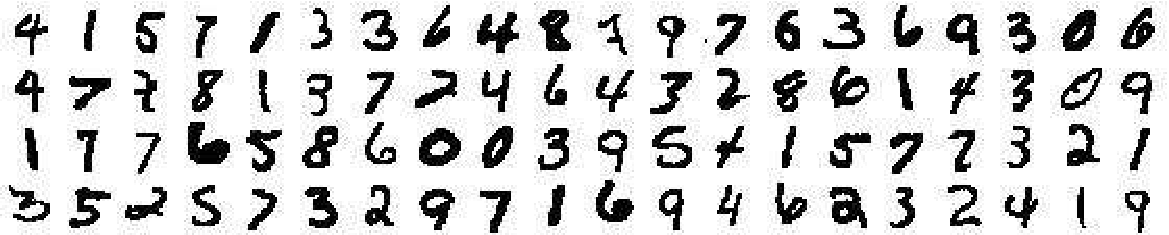
\includegraphics[width=6in]{figs/mnist.pdf}
\end{center}

\noindent
How can each such image be mapped to the corresponding digit? One approach is to
use {\it hand-coded rules}. This would involve two steps:
\begin{itemize}
\item Write subroutine to identify key features (such as loops) of an image.
\item Write a bunch of rules, like ``if there's a loop then it's not a 1,3,5 or 7''.
\end{itemize}
Both steps are problematic. As you can see from the examples above, real handwritten
digits are rife with deviations from ideal script, such as almost-loops. These 
variations can easily trip up a set of rigid rules. A much better idea is to 
{\it learn a classifier automatically from data}.

\subsection{The input space and the label space}

We want to create a classifier that takes an image $x$ and outputs a label $y$.
What are the spaces $\X$ and $\Y$ from which these images and labels are drawn?

The Post Office has made available a {\it training set} of $60{,}000$ digit-images. 
Each of these is a $28 \times 28$ greyscale image of a single digit. We can represent 
an image $x$ by a vector of 784 coordinates, one per pixel. The input space is then
$\X = \R^{784}$. The label space is, naturally, $\Y = \{0,1,\ldots, 9\}$. Thus the 
classifier we seek is a function $f: \X \rightarrow \Y$.

The training set can be written as $(x_1, y_1), \ldots, (x_n,y_n)$ where $n = 60{,}000$
and each $x_i \in \X$, $y_i \in \Y$. How can we use this data to find a good classifier
$f$?

\subsection{A nearest neighbor classifier}

Here's a simple classifier: for any image $x$, the label $f(x)$ is given by the 
following procedure.
\begin{itemize}
\item Find the $x_i$ that is closest to $x$ (out of $x_1, \ldots, x_n$).
\item Return $y_i$.
\end{itemize}
What is meant by ``closest to''? Well, we can use any notion of distance. One
natural option is just Euclidean distance. For two dimensional vectors 
$a = (a_1, a_2)$ and $b = (b_1, b_2)$, the Euclidean distance is given by the
familiar formula
$$ \|a - b\| \ = \ \sqrt{(a_1 - b_1)^2 + (a_2 - b_2)^2} .$$
A similar formula applies in higher dimensions. For $a,b \in \R^d$, we have
$$ \|a - b\| \ = \ \sqrt{\sum_{i=1}^d (a_i- b_i)^2} .$$

How good is this classifier? Is it always correct? Well, it is certainly
has zero error on the training set: that is, $f(x_i) = y_i$ for training 
points $(x_i, y_i)$. But $f$ might not be correct for other images $x$. 
How can we assess its accuracy?

To this end, the Post Office has also provided a separate {\it test set} of
different images and their labels. Any classifier can be tried out on this
test set to see what fraction of images it gets correct. The performance on
this test set is then a good indication of the performance of the classifier
in practice (using the standard theory of sampling). It turns out that
the classifier we have just constructed has an error rate of $23\%$ on the
test set.

Randomly guessing a label would have an error rate of $90\%$, so $23\%$ isn't 
too shabby, but it is certainly not good enough for the Post Office's purposes. 
How can we do better?

\subsection{Two improvements}

Euclidean distance is not really an ideal distance measure between images.
Consider two images that are identical, except that one is shifted slightly
to the right, or is rotated slightly, or is slightly thicker. The Euclidean
distance between these images will be substantial. It would be a lot more
sensible to compute the distance between two images $x$ and $x'$ as follows:
\begin{itemize}
\item First maximally ``align'' the two images by translating and rotating them.
\item Then compute Euclidean distance.
\end{itemize}

A further improvement is obtained by looking not just at the nearest neighbor
of $x$, but at the $k$ nearest neighbors (for some small value of $k$ like $7$),
and returning the most common label amongst these neighbors.

When these two changes are made, the error of the classifier on the test set 
drops below $1\%$.

\subsection{The computational complexity of finding the nearest neighbor}

Suppose points $x_1, \ldots, x_n$ lie in $\R^d$. How does one find the nearest
neighbor of a new point $x$? Here's the brute-force method:
\begin{itemize}
\item Compute all distances $\|x_i - x\|$.
\item Pick the $x_i$ for which this is smallest.
\end{itemize}
This algorithm takes time $O(n)$, which is prohibitive when $n$ is large.
We don't want to have to look through $60{,}000$ images just to classify
one new image!

There are two ways around this.
\begin{enumerate}
\item There are various data structures which enable efficient nearest neighbor search.
The most popular of these---spatial partition trees and hashing---rely heavily
on randomization, and can bring the search time down to $O(\log n)$.
\item Instead of using the entire training set, we can just pick a few representative
examples of each digit: these are called {\it prototypes}. However, the question of 
how to choose prototypes has still not been resolved satisfactorily.
\end{enumerate}

\section{Decision trees}

\subsection{Credit card fraud detection}

Credit card fraud is a massive problem. How can it be reduced, given that before
every transaction, the credit company has a brief moment in which to review the
details of the purchase and decline it if it is suspicious? Can a computer pick
out transactions that are likely to be fraudulent?

One approach is to ask a set of ``experts'' to hand-code some criteria, such as:
\begin{itemize}
\item Is the purchase amount more than twice the usual purchase price for this customer?
\item Is the purchase outside the customer's home area?
\item Has the customer bought other items of the same type over the past year?
\end{itemize}
This approach has many problems: there are far too many rules needed, and it is not 
clear how to set the constants in each rule (for instance, the ratio ``twice'' in the
first rule above), or how to weight the relative importance of the different rules.
A more promising strategy is to {\it learn} rules automatically from data.

\subsection{The input space and the label space}

Each input $x$ is the description of a credit card transaction. We can code it as
a vector with a large number of features (coordinates), for instance:
\begin{itemize}
\item Customer data
\begin{itemize}
\item Information about customer: sex, age, city of residence, etc.
\item Purchase history: for each category of purchases, typical dollar amount per purchase, number of purchases per year, number of purchases outside home area, etc.
\end{itemize}
\item Details of current purchase: type of item, dollar amount, location, does it fall into a standard ``dubious'' category (firearms, alcohol, ...), etc.
\item Relation of current purchase to prior purchase history: price of item divided by average price of similar items purchased over past year, etc.
\end{itemize}
Say these form a $d$-dimensional vector. Then $\X = \R^d$.
The label space is $\Y = \{+,-\}$ where ``$+$'' means the transaction is legitimate 
while ``$-$'' means it is fraudulent.

As always, we need a training set $(x_1,y_1), \ldots, (x_n,y_n)$, and to evaluate our
classifier, we will also need a (typically smaller) test set.

\subsection{Classification by decision tree}

A decision tree is a binary tree where each internal node checks a specific coordinate
of the input $x$, to see whether it lies in a specified range. Each leaf of the tree
is a label, $+$ or $-$. To classify an input $x$, you answer the question at the root,
then move to either the left or right child, depending on the answer; and continue this
way until you reach a leaf.

Here's a toy example of a decision tree.

\begin{center}
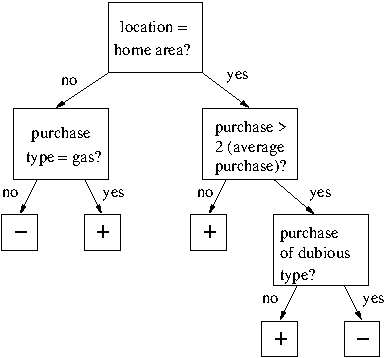
\includegraphics[width=3.5in]{figs/decision.pdf}
\end{center}

\noindent
(We assume the vectorial representation is sufficiently rich that each question can be 
answered by looking at a single coordinate of $x$.) 

How can such a tree be learned from data? The answer is, by building it top-down,
adding nodes greedily to {\it reduce uncertainty}.

\subsection{Learning a decision tree}

Suppose the training set has 10000 points, with
\begin{enumerate}
\item[] $6000$ legitimate ($+$)
\item[] $4000$ fraudulent ($-$)
\end{enumerate}
If we were allowed just one node, it would be a leaf with label ``$+$'':

\begin{center}
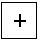
\includegraphics[width=0.3in]{figs/decision1.pdf}
\end{center}

\noindent
This has an error rate of $40\%$ on the training data.

Now suppose we were allowed just one question. For instance, we might ask whether
the location of the purchase is in the customer's home area. The answer to this 
question, yes or no, splits the training set into two subsets. Let's say the
breakdown is as follows.

\begin{center}
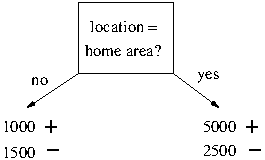
\includegraphics[width=2.5in]{figs/decision2.pdf}
\end{center}

\noindent
Then on the left leaf we'd predict ``$-$'' while on the right we'd predict
``$+$'', yielding:

\begin{center}
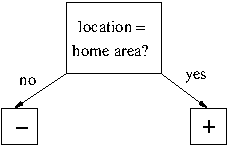
\includegraphics[width=2.25in]{figs/decision3.pdf}
\end{center}

A quarter of the training points end up in the left leaf, and amongst them the
error rate is $2/5$. Three-quarters of the points end up in the right leaf, and
amongst them the error rate is $1/3$. Thus the overall error rate is now
$$ \frac{1}{4} \cdot \frac{2}{5} + \frac{3}{4} \cdot \frac{1}{3} 
\ = \ \frac{7}{20},$$
or $35\%$, less than before!

So asking this particular question reduces the error rate. We should pick the
question that {\it most} reduces the error, and then recurse on the leaves. Here's
the procedure:
\begin{itemize}
\item Start with a single leaf node for all the training points.
\item Repeat:
\begin{itemize}
\item Pick a leaf that has significant error and contains quite a lot of training points.
(If there is no such leaf, halt.)
\item Split it by asking a question that maximally reduces error within the leaf.
\end{itemize}
\end{itemize}

\section{Linear classifiers}

\subsection{Document classification}

The internet brings with it a host of important {\it document classification} tasks.
For instance,
\begin{itemize}
\item Is an email message spam or not? Input: email, label: $+$ (legitimate) or $-$ (spam).
\item {\it Sentiment detection.} Is an article (such as a review) positive/favorable about 
its subject or negative/unfavorable? Input: article, label: $+$ (favorable) or $-$ 
(unfavorable).
\item Is the text on a webpage pornographic (in which case Google wouldn't want to return
it) or not? Input: text on webpage, label: $+$ (suitable for general audiences) or $-$ 
(pornographic).
\end{itemize}

As always, one approach towards solving these problems is to hand-code rules. For instance, 
given the large volume of spam that seems to involve getting money out of Nigerian bank 
accounts, a possible rule for spam might be to flag emails containing the words 
``Nigeria'' and ``bank''. But vast numbers of such rules are needed, and they are
constantly changing. It is more convenient and reliable to {\it learn} rules 
automatically from data.

\subsection{The input space $\X$ and label space $\Y$}

A document is a sequence of words, and different documents have different lengths. How can
they be represented as vectors of fixed dimension? The standard way to do so is the 
{\it bag of words} model.

Start by picking a fixed list of words, for instance, $50{,}000$ of the most common words
in English. Now represent each document as a vector $x$ with $50{,}000$ coordinates, each
associated with a particular word. That coordinate records how many times the word occurs
in the document. For example, the really short piece of text
\begin{quote}
a rose is a rose
\end{quote}
would correspond to a vector in which the coordinate for ``a'' has value 2, the
coordinate for ``is'' has value 1, the coordinate for ``rose'' has value 2,
and the remaining $49,997$ coordinates are zero.

Thus $\X = \R^{50000}$ and $\Y = \{+,-\}$. As always, we will need a training set
$(x_1, y_1), \ldots, (x_n, y_n)$, to guide our choice of classifier, as well as a 
test set on which to evaluate our final classifier.

\subsection{Linear classifiers}

Suppose the data lie in $\R^2$ instead of $\R^{50000}$. Then we can plot each training
point $x_i$ and annotate it with its label $y_i$.

\begin{center}

\includegraphics[width=2in]{figs/linear1.pdf}
\end{center}

A {\it linear classifier} $f: \R^2 \rightarrow \{+,-\}$ is simply a line with $+$ on one
side and $-$ on the other side. Future points can be classified by which side of the line
they lie on.

\begin{center}
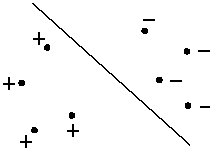
\includegraphics[width=2in]{figs/linear2.pdf}
\end{center}

\noindent
This also works in higher dimension---that is, when $\X = \R^d$---but instead of a line
we have a $(d-1)$-dimensional hyperplane. For instance, when $d=3$ the boundary between
positive and negative is a plane.

\subsection{Learning a linear classifier}

Given a training set $(x_1, y_1), \ldots, (x_n, y_n)$, we'd like to find a linear
function $f$ that correctly classifies all the points, that is, $f(x_i) = y_i$ 
for all $i$. There are two complications, however.

First, in the example above there are infinitely many solutions: infinitely many
ways to draw a line between the positive and negative points. Which one should be
used? A popular choice is to pick the line that is most squarely in the middle
(according to a precise criterion), something like:

\begin{center}

\includegraphics[width=2in]{figs/linear3.pdf}
\end{center}

A second problem is that sometimes there is no linear classifier that gets all
the points correct:

\begin{center}
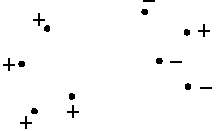
\includegraphics[width=2in]{figs/linear4.pdf}
\end{center}

\noindent
In such cases, we'd like to pick a linear function that makes the fewest mistakes 
possible (or some approximation thereof). Both these problems are handled by the
widely-used {\it support vector machine}. We won't get into the details here, but
there are plenty of software packages that will take as input a data set and 
produce a linear classifier from it.

In fact, there are further extensions that allow the boundary between the two 
classes to be nonlinear (quadratic, or cubic, or even pretty arbitrary), and 
that allow non-vector data such as DNA sequences or trees!



        % 7.tex

\end{document}




